\documentclass{uetgraduation}
\usepackage{array}
\usepackage{amssymb}
\usepackage{subcaption}
\usepackage[
    colorlinks=true,
    linkcolor=black,
    citecolor=black,
    urlcolor=blue,
    bookmarks=true,
    bookmarksopen=true
]{hyperref}

\begin{document}
% ---------------------------------------------
% 1. Thông tin trang bìa
% ---------------------------------------------
\studentname{Đoàn Văn Giáp}
\title{Tác động của phần thưởng nội tại đến quá trình khám phá trong Học tăng cường}
\documenttype{Báo cáo dự án công nghệ}
\major{Công nghệ thông tin}
\year{2025}
\supervisor{TS. Nguyễn Thị Thủy}

\makecovers % Tạo các trang bìa

% ---------------------------------------------
% 2. Các trang Tóm tắt, Lời cam đoan, Cảm ơn
% ---------------------------------------------

\begin{preamble}{Lời cam đoan}
Em là Đoàn Văn Giáp, sinh viên lớp QH-2022-I/CQ-I-IT1 khóa K67, ngành Công nghệ thông tin tại trường Đại học Công Nghệ - Đại học Quốc gia Hà Nội.\\
Em xin cam đoan: Dự án công nghệ với đề tài ``Tác động của phần thưởng nội tại đến quá trình khám phá trong Học tăng cường'' trong báo cáo này là công trình nghiên cứu do bản thân em tìm hiểu, thực hiện, và đánh giá. Các nội dung có trình bày trong bản báo cáo đều được thực hiện một cách chính xác và xác thực.\\
Các thông tin có trong báo cáo là có cơ sở và các nội dung được trích dẫn từ các tài liệu khác đều được ghi rõ nguồn tham khảo. Em xin chịu trách nhiệm về lời
cam đoan này.

\vspace{2cm}

\begin{flushright}
Hà Nội, ngày 21 tháng 12 năm 2025

\vspace{1\baselineskip}

\begin{minipage}{6cm}
\centering
Sinh viên

\vspace{4\baselineskip}

Đoàn Văn Giáp
\end{minipage}
\end{flushright}


\end{preamble}

\begin{preamble}{Lời cảm ơn}
Em xin chân thành cảm ơn TS. Nguyễn Thị Thủy đã tận tình hướng dẫn, chỉ bảo và tạo điều kiện thuận lợi để em hoàn thành báo cáo này. 

Em cũng xin gửi lời cảm ơn đến các thầy cô trong Khoa Công nghệ Thông tin, Trường Đại học Công nghệ, Đại học Quốc gia Hà Nội đã trang bị cho em những kiến thức nền tảng quý báu trong suốt quá trình học tập.
\end{preamble}

\begin{preamble}{Tóm tắt}
Trong lĩnh vực Học tăng cường (Reinforcement Learning), vấn đề khám phá (exploration) trong môi trường có phần thưởng thưa thớt (sparse reward) là một thách thức lớn. Các chiến lược khám phá cổ điển thường thất bại do không nhận được tín hiệu phản hồi đủ sớm để hướng dẫn tác tử. Báo cáo này tập trung nghiên cứu hiệu quả của phương pháp phần thưởng nội tại (Intrinsic Rewards) dựa trên kỹ thuật Random Network Distillation (RND) kết hợp với thuật toán Proximal Policy Optimization (PPO).

Nghiên cứu thực hiện khảo sát tác động của các hệ số phần thưởng nội tại ($\lambda$) khác nhau bao gồm 1, 0.1 và 0.01 lên hiệu suất của tác tử. Môi trường thực nghiệm được lựa chọn là bộ MiniGrid với các bài toán đòi hỏi khả năng điều hướng và lập kế hoạch, bao gồm DoorKey (kích thước 5x5, 6x6, 8x8), LavaCrossing (S9N1, S9N2, S9N3) và KeyCorridor (S3R1, S3R2). Mục tiêu là đánh giá khả năng của RND trong việc thúc đẩy tác tử khám phá các trạng thái mới và hoàn thành tác vụ khi phần thưởng ngoại lai rất hiếm gặp.

\textit{\textbf{Từ khóa:} Học tăng cường, Phần thưởng nội tại, PPO, RND, MiniGrid.}
\end{preamble}

% ---------------------------------------------
% 3. Mục lục và Danh sách
% ---------------------------------------------
\begin{contentlisting}

\tableofcontents % Mục lục
\listoffigures % Danh sách hình vẽ
\listoftables % Danh sách bảng

\begin{contentlistingsection}{Danh mục các từ viết tắt}

\begin{center}
\renewcommand{\arraystretch}{1.3}
\setlength{\tabcolsep}{8pt}

\begin{tabular}{|
    >{\centering\arraybackslash}m{1cm}
    |>{\centering\arraybackslash}m{2.5cm}
    |>{\raggedright\arraybackslash}m{5cm}
    |>{\raggedright\arraybackslash}m{5cm}|
}
\hline
\textbf{STT} & \textbf{Từ viết tắt} & \textbf{Cụm từ đầy đủ} & \textbf{Cụm từ tiếng Việt} \\
\hline
1 & RL   & Reinforcement Learning & Học tăng cường \\
\hline
2 & MDP  & Markov Decision Process & Quá trình quyết định Markov \\
\hline
3 & PPO  & Proximal Policy Optimization & Tối ưu hóa chính sách lân cận \\
\hline
4 & RND  & Random Network Distillation & Chưng cất mạng ngẫu nhiên \\
\hline
5 & TRPO & Trust Region Policy Optimization & Tối ưu hóa chính sách vùng tin cậy \\
\hline
6 & ICM  & Intrinsic Curiosity Module & Mô-đun tò mò nội tại \\
\hline
7 & MSE  & Mean Squared Error & Sai số bình phương trung bình \\
\hline
8 & DIAYN & Diversity Is All You Need & Đa dạng là tất cả những gì bạn cần \\
\hline
9 & SAC  & Soft Actor-Critic & Tác tử-Phê bình mềm \\
\hline
10 & MLP & Multi-Layer Perceptron & Mạng nơ-ron đa lớp \\
\hline
\end{tabular}
\end{center}

\end{contentlistingsection}

\end{contentlisting}

% ---------------------------------------------
% 4. Nội dung chính
% ---------------------------------------------

% =============================================
% CHƯƠNG 1: GIỚI THIỆU
% =============================================
\chapter{Giới thiệu}

\section{Động lực nghiên cứu}

Trong thập kỷ qua, lĩnh vực Học tăng cường (Reinforcement Learning - RL) đã chứng kiến sự phát triển vượt bậc, đánh dấu bởi những thành tựu mang tính đột phá trong việc giải quyết các bài toán ra quyết định tuần tự phức tạp. Từ việc các hệ thống như AlphaGo của Google DeepMind đánh bại con người trong trò chơi cờ vây, cho đến các tác nhân ảo làm chủ các trò chơi điện tử phức tạp như Dota 2 hay StarCraft II, RL đã chứng minh tiềm năng to lớn trong việc xây dựng trí tuệ nhân tạo có khả năng tự học hỏi. Cơ chế cốt lõi của RL dựa trên sự tương tác thử và sai (trial-and-error) giữa một tác nhân (agent) và môi trường, trong đó tác nhân học cách tối ưu hóa một chính sách (policy) để cực đại hóa tổng phần thưởng tích lũy (cumulative reward) theo thời gian.

Tuy nhiên, việc áp dụng RL vào các bài toán thực tế hoặc các môi trường mô phỏng phức tạp vẫn đối mặt với một rào cản lớn: vấn đề phần thưởng thưa (sparse reward problem). Trong các thiết lập RL tiêu chuẩn, hàm phần thưởng thường được thiết kế để cung cấp tín hiệu phản hồi liên tục cho tác nhân. Tuy nhiên, trong nhiều bài toán thực tế như điều hướng robot trong mê cung, lắp ráp chi tiết máy, hay khám phá không gian mạng, tín hiệu phần thưởng ngoại sinh (extrinsic reward) - tức phần thưởng do môi trường quy định - thường rất hiếm hoặc chỉ xuất hiện khi tác nhân hoàn thành trọn vẹn một chuỗi hành động phức tạp. Ví dụ, trong bài toán Montezuma's Revenge của bộ Atari, tác nhân có thể phải thực hiện hàng trăm bước di chuyển chính xác qua nhiều phòng, tránh chướng ngại vật và thu thập vật phẩm trước khi nhận được bất kỳ điểm số nào. Trong khoảng thời gian dài không có tín hiệu phản hồi này, các thuật toán RL truyền thống dựa trên $\epsilon$-greedy hoặc entropy regularization thường thất bại do không nhận được gradient có ý nghĩa để cập nhật trọng số mạng nơ-ron. Tác nhân sẽ rơi vào trạng thái di chuyển ngẫu nhiên vô định mà không thể hội tụ về lời giải tối ưu.

Để khắc phục hạn chế này, các nhà nghiên cứu đã tìm đến cảm hứng từ tâm lý học hành vi, cụ thể là khái niệm ``động lực nội tại'' (intrinsic motivation). Ý tưởng chủ đạo là trang bị cho tác nhân khả năng tự tạo ra phần thưởng cho chính mình (intrinsic reward) dựa trên sự tò mò (curiosity) hoặc mong muốn khám phá những điều mới lạ, độc lập với phần thưởng ngoại sinh. Phần thưởng nội tại này đóng vai trò như một tín hiệu dẫn đường, khuyến khích tác nhân khám phá các trạng thái chưa từng ghé thăm hoặc các vùng không gian trạng thái mà tác nhân chưa hiểu rõ. Tổng phần thưởng mà tác nhân tối ưu hóa tại mỗi bước thời gian $t$ sẽ là tổng trọng số của phần thưởng ngoại sinh ($r_e$) và phần thưởng nội tại ($r_i$), thường được biểu diễn dưới dạng:
\begin{equation}
R_t = r_{e,t} + \lambda r_{i,t}
\end{equation}
Trong đó, $\lambda$ là hệ số điều chỉnh (scaling coefficient) xác định mức độ ưu tiên giữa việc khai thác mục tiêu của môi trường và nhu cầu khám phá nội tại.

Trong số các phương pháp tạo sinh phần thưởng nội tại, kỹ thuật Chưng cất Mạng Ngẫu nhiên (Random Network Distillation - RND) được giới thiệu bởi Burda và cộng sự (2018) đã nổi lên như một giải pháp hiệu quả và ổn định, đặc biệt cho các môi trường có không gian quan sát chiều cao như hình ảnh. Khác với các phương pháp dựa trên mô hình động lực học (dynamics-based models) vốn yêu cầu dự đoán trạng thái tương lai của môi trường - một tác vụ khó khăn và dễ bị nhiễu bởi các yếu tố ngẫu nhiên (vấn đề ``Noisy-TV''), RND tiếp cận vấn đề theo hướng đơn giản hơn. RND sử dụng hai mạng nơ-ron: một mạng đích (target network) được khởi tạo ngẫu nhiên và cố định trọng số, và một mạng dự đoán (predictor network) được huấn luyện để sao chép đầu ra của mạng đích trên các trạng thái mà tác nhân quan sát được. Phần thưởng nội tại được định nghĩa là sai số bình phương trung bình (MSE) giữa đầu ra của hai mạng. Khi tác nhân ghé thăm một trạng thái quen thuộc, mạng dự đoán đã được huấn luyện trên trạng thái đó nên sai số sẽ thấp. Ngược lại, tại các trạng thái mới lạ, sai số sẽ cao, tạo ra tín hiệu phần thưởng thúc đẩy tác nhân quay lại hoặc khám phá sâu hơn vùng không gian đó.

Mặc dù RND kết hợp với các thuật toán tối ưu hóa chính sách như Proximal Policy Optimization (PPO) đã đạt được những kết quả ấn tượng, một vấn đề thực tiễn quan trọng vẫn chưa được giải quyết triệt để: sự nhạy cảm của thuật toán đối với hệ số điều chỉnh $\lambda$. Trong phương trình tổng phần thưởng, $\lambda$ đóng vai trò cân bằng giữa ``lòng tham'' muốn đạt điểm số cao (khai thác) và ``sự tò mò'' muốn tìm hiểu môi trường (khám phá). Các nghiên cứu trước đây, điển hình là công trình của Andres và cộng sự (2022), đã chỉ ra rằng hiệu năng của các thuật toán dựa trên động lực nội tại phụ thuộc rất lớn vào các lựa chọn thiết kế và siêu tham số. Tuy nhiên, đa số các công trình thường cố định $\lambda$ hoặc coi nó là một tham số phụ, mà thiếu đi các phân tích hệ thống về tác động của độ lớn $\lambda$ đối với hành vi hội tụ của tác nhân.

Nếu $\lambda$ quá nhỏ, tín hiệu khám phá sẽ bị chìm nghỉm trong nhiễu hoặc không đủ mạnh để đẩy tác nhân ra khỏi các vùng tối ưu cục bộ, khiến thuật toán quay về hành vi của PPO thuần túy và thất bại trong môi trường phần thưởng thưa. Ngược lại, nếu $\lambda$ quá lớn, tác nhân có thể bị ``nghiện'' phần thưởng nội tại (intrinsic reward hacking), dẫn đến việc nó chỉ tập trung tìm kiếm các trạng thái mới lạ mà lãng quên nhiệm vụ chính, hoặc gây ra sự mất ổn định (instability) trong quá trình huấn luyện do hàm mục tiêu thay đổi quá nhanh (non-stationary objective). Khoảng trống nghiên cứu này đặt ra nhu cầu cấp thiết về một phân tích thực nghiệm chuyên sâu nhằm hiểu rõ mối quan hệ nhân quả giữa hệ số $\lambda$ và hiệu quả khám phá.

Xuất phát từ bối cảnh trên, khóa luận này tập trung nghiên cứu đề tài: ``Tác động của phần thưởng nội tại đến quá trình khám phá trong học tăng cường'', với trọng tâm là phân tích thực nghiệm ảnh hưởng của hệ số $\lambda$ khi tích hợp module RND vào thuật toán PPO.

\section{Các nghiên cứu liên quan}

Để đặt nghiên cứu này vào bối cảnh học thuật phù hợp, phần này sẽ tổng quan các hướng tiếp cận chính trong việc giải quyết bài toán khám phá (exploration) thông qua phần thưởng nội tại. Các phương pháp hiện có có thể được phân loại thành ba nhóm chính: phương pháp dựa trên đếm (count-based), phương pháp dựa trên lỗi dự đoán (prediction-based), và phương pháp dựa trên đa dạng kỹ năng (skill-based/competence-based).

\subsection{Phương pháp dựa trên đếm (Count-based Exploration)}

Phương pháp dựa trên đếm là cách tiếp cận trực quan nhất đối với vấn đề khám phá. Trong bối cảnh RL dạng bảng (tabular RL) với không gian trạng thái nhỏ và rời rạc, các thuật toán như MBIE-EB (Model-Based Interval Estimation - Exploration Bonus) đếm số lần tác nhân ghé thăm một trạng thái $s$, ký hiệu là $N(s)$. Phần thưởng nội tại thường được tính tỷ lệ nghịch với căn bậc hai của số lần ghé thăm: $r_i \propto 1/\sqrt{N(s)}$. Cơ chế này khuyến khích tác nhân ưu tiên các trạng thái ít được ghé thăm, giúp giảm độ bất định của mô hình về môi trường.

Tuy nhiên, khi áp dụng vào các bài toán có không gian trạng thái lớn hoặc liên tục (như đầu vào là hình ảnh pixel), việc đếm trực tiếp trở nên bất khả thi vì hầu hết các trạng thái sẽ chỉ xuất hiện duy nhất một lần trong suốt quá trình huấn luyện ($N(s)$ luôn bằng 0 hoặc 1). Để giải quyết vấn đề này, Bellemare và cộng sự (2016) đã đề xuất khái niệm ``pseudo-counts'' (bộ đếm giả), sử dụng các mô hình mật độ (density models) như Context-Tree Switching (CTS) để ước lượng xác suất xuất hiện của trạng thái, từ đó suy ra số lần ghé thăm tương đương.

Một hướng tiếp cận khác để mở rộng phương pháp đếm là thực hiện đếm trong không gian đặc trưng (feature space) thay vì không gian quan sát thô. Công trình của Martin và cộng sự (2017) đề xuất thuật toán $\phi$-EB, trong đó họ xây dựng mô hình mật độ dựa trên các đặc trưng được học bởi mạng nơ-ron xấp xỉ hàm giá trị. Bằng cách đo lường độ mới lạ trong không gian đặc trưng, phương pháp này cho phép tổng quát hóa việc đếm: các trạng thái có đặc trưng tương tự nhau sẽ chia sẻ số lần đếm, giúp tác nhân nhận diện được sự quen thuộc ngay cả khi quan sát pixel có sự thay đổi nhỏ. Mặc dù các phương pháp dựa trên đếm có nền tảng lý thuyết vững chắc, chúng thường gặp khó khăn trong việc mở rộng (scalability) và đòi hỏi chi phí tính toán lớn để duy trì các mô hình mật độ phức tạp.

\subsection{Phương pháp dựa trên lỗi dự đoán (Prediction-based Exploration)}

Đây là nhóm phương pháp phổ biến nhất trong Deep RL hiện đại, định nghĩa sự tò mò (curiosity) là sai số của tác nhân khi cố gắng dự đoán tương lai.

Một trong những công trình tiên phong là Intrinsic Curiosity Module (ICM) do Pathak và cộng sự (2017) đề xuất. ICM giải quyết vấn đề không gian chiều cao bằng cách học một không gian đặc trưng nghịch đảo (inverse dynamics feature space). Thay vì dự đoán từng pixel của khung hình tiếp theo (vốn rất khó và lãng phí tài nguyên), ICM huấn luyện một mạng nơ-ron để dự đoán hành động $a_t$ mà tác nhân đã thực hiện để chuyển từ trạng thái $s_t$ sang $s_{t+1}$. Quá trình này buộc mạng nơ-ron phải học các đặc trưng liên quan đến sự kiểm soát của tác nhân, đồng thời loại bỏ các yếu tố nhiễu nền không thể kiểm soát (như lá cây bay trong gió hay nhiễu trắng trên màn hình TV). Phần thưởng nội tại sau đó được tính bằng sai số dự đoán của một mô hình thuận (forward model) hoạt động trong không gian đặc trưng này.

Tuy nhiên, ICM vẫn gặp phải những thách thức nhất định khi đối mặt với các môi trường có tính ngẫu nhiên cao (stochasticity). Burda và cộng sự (2018) đã chỉ ra vấn đề ``Noisy-TV'': nếu môi trường chứa một chiếc TV chuyển kênh ngẫu nhiên, các phương pháp dựa trên dự đoán động lực học (như ICM) sẽ bị thu hút mãi mãi vào chiếc TV đó vì sai số dự đoán luôn cao, bất kể tác nhân quan sát bao lâu. Để khắc phục, họ đề xuất Random Network Distillation (RND). RND thay đổi bài toán dự đoán động lực học thành bài toán dự đoán đầu ra của một mạng nơ-ron đích cố định (fixed target network). Vì mạng đích là tất định (deterministic), RND triệt tiêu được vấn đề Noisy-TV. Khi tác nhân quan sát một trạng thái nhiều lần, mạng dự đoán sẽ học được cách mô phỏng mạng đích, làm giảm phần thưởng nội tại, bất kể trạng thái đó có chứa nhiễu ngẫu nhiên hay không. Sự đơn giản và khả năng mở rộng của RND đã biến nó thành một phương pháp chuẩn mực (baseline) cho các bài toán khám phá khó như Montezuma's Revenge.

\subsection{Phương pháp dựa trên đa dạng kỹ năng (Skill-based Exploration)}

Một hướng tiếp cận khác không tập trung trực tiếp vào việc tối đa hóa sai số dự đoán hay số lần ghé thăm, mà hướng tới việc học một tập hợp các kỹ năng (skills) đa dạng. Công trình tiêu biểu cho hướng này là ``Diversity is All You Need'' (DIAYN) của Eysenbach và cộng sự (2018). DIAYN khuyến khích tác nhân học các chính sách (policies) có thể phân biệt được với nhau thông qua việc tối đa hóa thông tin tương hỗ (mutual information) giữa trạng thái và một biến tiềm ẩn đại diện cho kỹ năng. Mục tiêu là phát triển các hành vi đa dạng mà không cần hàm phần thưởng ngoại sinh.

Tuy nhiên, hiệu quả thực sự của các phương pháp dựa trên kỹ năng trong việc giải quyết bài toán khám phá thuần túy (pure exploration) vẫn còn là chủ đề tranh luận. Một nghiên cứu thực nghiệm gần đây của Kayal và cộng sự (2025) với tiêu đề ``The impact of intrinsic rewards on exploration in Reinforcement Learning'' đã so sánh DIAYN với các phương pháp đếm trạng thái và ICM trên môi trường MiniGrid. Kết quả của họ chỉ ra rằng, mặc dù DIAYN học được các hành vi đa dạng, nó không nhất thiết dẫn đến việc bao phủ không gian trạng thái (state coverage) tốt hơn. Trong các môi trường lưới đơn giản, phương pháp đếm trạng thái (State Count) thậm chí còn vượt trội hơn DIAYN về khả năng khám phá. Điều này gợi ý rằng sự đa dạng về hành vi (behavioral diversity) không đồng nghĩa với hiệu quả khám phá không gian (spatial exploration), và việc lựa chọn phương pháp phụ thuộc rất lớn vào đặc thù của môi trường.

\subsection{Các nghiên cứu đánh giá và phân tích siêu tham số}

Bên cạnh việc đề xuất các thuật toán mới, các nghiên cứu đánh giá (evaluation studies) đóng vai trò quan trọng trong việc hiểu rõ hành vi của các thành phần thuật toán. Andres và cộng sự (2022) trong công trình ``An Evaluation Study of Intrinsic Motivation Techniques applied to Reinforcement Learning over Hard Exploration Environments'' đã thực hiện một khảo sát toàn diện về các kỹ thuật động lực nội tại. Nghiên cứu của họ nhấn mạnh rằng hiệu năng của các thuật toán như RND hay ICM cực kỳ nhạy cảm với các lựa chọn thiết kế như: kiến trúc mạng nơ-ron, cơ chế chuẩn hóa phần thưởng, và đặc biệt là cách kết hợp trọng số giữa phần thưởng nội tại và ngoại sinh.

Đáng chú ý, Andres và cộng sự chỉ ra một khoảng trống nghiên cứu quan trọng: ảnh hưởng của các siêu tham số này thường bị bỏ qua hoặc không được phân tích tách biệt trong các công bố gốc. Hầu hết các nghiên cứu chỉ báo cáo kết quả với bộ siêu tham số tốt nhất mà không minh họa sự suy giảm hiệu năng khi các tham số này thay đổi. Ví dụ, sự tác động của cơ chế ``episodic count'' (đếm trong tập) so với ``lifelong count'' (đếm trong suốt quá trình huấn luyện) đối với RND là rất lớn nhưng ít được thảo luận chi tiết.

Tổng hợp lại, mặc dù RND là một phương pháp mạnh mẽ, và các nghiên cứu đánh giá đã bắt đầu chú ý đến vai trò của siêu tham số, vẫn thiếu một phân tích thực nghiệm chuyên sâu và cô lập về tác động của hệ số cân bằng $\lambda$ cụ thể trong bối cảnh tích hợp với PPO. Khóa luận này nhằm mục đích điền vào khoảng trống đó, cung cấp các bằng chứng thực nghiệm về độ nhạy của thuật toán đối với $\lambda$ và đề xuất các ngưỡng giá trị phù hợp.

\section{Mục tiêu và đóng góp của nghiên cứu}

Mục tiêu cốt lõi của khóa luận là thực hiện một phân tích thực nghiệm hệ thống về tác động của phần thưởng nội tại, cụ thể là thông qua phương pháp Random Network Distillation (RND), đối với hiệu quả khám phá của thuật toán Proximal Policy Optimization (PPO) trong các môi trường có phần thưởng thưa. Nghiên cứu tập trung vào việc làm rõ hành vi của tác nhân dưới các chế độ trọng số phần thưởng nội tại khác nhau, từ đó rút ra các nhận định về sự cân bằng giữa khám phá và khai thác.

Các đóng góp chính của khóa luận được tóm tắt như sau:
\begin{itemize}
    \item Tích hợp hệ thống: Xây dựng và tích hợp thành công module RND vào thuật toán cơ sở PPO như một thành phần độc lập (plugin module). Kiến trúc này cho phép linh hoạt bật/tắt hoặc điều chỉnh cường độ của tín hiệu nội tại mà không làm thay đổi cấu trúc cốt lõi của thuật toán tối ưu hóa chính sách.
    
    \item Phân tích thực nghiệm về hệ số $\lambda$: Thực hiện một loạt các thí nghiệm so sánh có kiểm soát (controlled experiments) giữa PPO thuần túy (baseline) và PPO tích hợp RND với các hệ số điều chỉnh $\lambda$ khác nhau ($\lambda \in \{1, 0.1, 0.01\}$). Đây là đóng góp trọng tâm nhằm trả lời câu hỏi về độ nhạy của thuật toán đối với độ lớn của phần thưởng nội tại, một vấn đề chưa được khai thác sâu trong các công bố gốc của Burda và cộng sự (2018).
    
    \item Đánh giá đa chiều: Phân tích định lượng và định tính ảnh hưởng của $\lambda$ đến tốc độ hội tụ (convergence rate) và độ bao phủ không gian trạng thái (state coverage). Kết quả phân tích sẽ làm rõ sự đánh đổi (trade-off): $\lambda$ lớn giúp khám phá nhanh nhưng có thể gây mất ổn định hội tụ, trong khi $\lambda$ nhỏ giúp ổn định nhưng có thể không vượt qua được rào cản phần thưởng thưa.
    
    \item Kiểm chứng thực tiễn: Cung cấp các bằng chứng thực nghiệm củng cố cho các nhận định lý thuyết trong nghiên cứu của Andres và cộng sự (2022) về tầm quan trọng của việc tinh chỉnh siêu tham số trong các thuật toán động lực nội tại. Nghiên cứu khẳng định lại rằng không có một giá trị $\lambda$ nào là tối ưu cho mọi bài toán, nhưng việc hiểu rõ hành vi của nó cho phép các kỹ sư RL lựa chọn chiến lược tốt hơn.
\end{itemize}

Cần nhấn mạnh rằng, phạm vi của khóa luận này tập trung vào phân tích thực nghiệm và đánh giá độ nhạy của thuật toán hiện có, không hướng tới việc đề xuất một cấu trúc mạng mới hay tuyên bố phát minh ra một thuật toán khám phá mới. Các kết quả thu được sẽ đóng vai trò là tài liệu tham khảo kỹ thuật cho việc ứng dụng PPO và RND trong các bài toán thực tế.

% =============================================
% CHƯƠNG 2: NỀN TẢNG LÝ THUYẾT
% =============================================
\chapter{Nền tảng lý thuyết}

\section{Học tăng cường}

\subsection{Quá trình quyết định Markov (MDP)}
% TODO: Viết nội dung

\subsection{Chính sách (Policy)}
% TODO: Viết nội dung

\subsection{Phần thưởng và hàm lợi ích tích lũy (Reward \& Return)}
% TODO: Viết nội dung

\subsection{Hàm giá trị (Value Function) và Hàm lợi thế (Advantage Function)}
% TODO: Viết nội dung

\subsection{Mục tiêu của học tăng cường}
% TODO: Viết nội dung

\subsection{Phân loại phương pháp học tăng cường}
% TODO: Viết nội dung

\section{Thuật toán Proximal Policy Optimization (PPO)}

\subsection{Phương pháp Policy Gradient}
% TODO: Viết nội dung

\subsection{Kiến trúc Actor–Critic}
% TODO: Viết nội dung

\subsection{Hàm mục tiêu Clipped Surrogate Objective}
% TODO: Viết nội dung

\subsection{Ước lượng Advantage và Generalized Advantage Estimation (GAE)}
% TODO: Viết nội dung

\subsection{Quy trình huấn luyện PPO}
% TODO: Viết nội dung

\section{Vấn đề khám phá trong học tăng cường}

\subsection{Exploration vs Exploitation}
% TODO: Viết nội dung

\subsection{Sparse reward problem}
% TODO: Viết nội dung

\subsection{Hạn chế của exploration ngẫu nhiên}
% TODO: Viết nội dung

\section{Phần thưởng nội tại (Intrinsic Reward)}
% TODO: Viết nội dung

\section{Mạng chưng cất ngẫu nhiên (Random Network Distillation - RND)}

\subsection{Động lực và ý tưởng của RND}
% TODO: Viết nội dung

\subsection{Kiến trúc mạng RND}
% TODO: Viết nội dung

\subsection{Cơ chế sinh phần thưởng nội tại}
% TODO: Viết nội dung

\subsection{Chuẩn hóa quan sát và phần thưởng (Observation \& Reward Normalization)}
% TODO: Viết nội dung

\subsection{Quy trình huấn luyện RND}
% TODO: Viết nội dung

\subsection{Hệ số điều chỉnh phần thưởng nội tại trong RND}
% TODO: Viết nội dung

% =============================================
% CHƯƠNG 3: PHƯƠNG PHÁP ĐỀ XUẤT
% =============================================
\chapter{Phương pháp đề xuất}

\section{Tổng quan kiến trúc phương pháp}
% TODO: Viết nội dung

\section{Thiết kế Module RND}
% TODO: Viết nội dung

\section{Cơ chế tích hợp phần thưởng (Reward Integration)}
% TODO: Viết nội dung

\section{Quy trình huấn luyện PPO + RND}
% TODO: Viết nội dung

% =============================================
% CHƯƠNG 4: THỰC NGHIỆM VÀ ĐÁNH GIÁ
% =============================================
\chapter{Thực nghiệm và đánh giá}

\section{Câu hỏi nghiên cứu}
% TODO: Viết nội dung

\section{Quy trình thực nghiệm}

\subsection{Môi trường và cấu hình thực nghiệm}

\begin{table}{Siêu tham số PPO}
\centering
\begin{tabular}{|l|c|l|}
\hline
\textbf{Tham số} & \textbf{Giá trị} & \textbf{Mô tả} \\
\hline
$\gamma$ & 0.99 & Hệ số chiết khấu \\
\hline
$\epsilon_{clip}$ & 0.2 & Ngưỡng clipping cho PPO \\
\hline
$K_{epochs}$ & 80 & Số epoch cập nhật mỗi lần update \\
\hline
$\alpha_{actor}$ & 0.0003 & Learning rate của Actor \\
\hline
$\alpha_{critic}$ & 0.001 & Learning rate của Critic \\
\hline
Update frequency & 4000 steps & Tần suất cập nhật policy \\
\hline
Max timesteps & $10^6$ & Tổng số bước huấn luyện \\
\hline
Max episode length & 1000 & Độ dài tối đa mỗi episode \\
\hline
\end{tabular}
\end{table}

\begin{table}{Siêu tham số RND}
\centering
\begin{tabular}{|l|c|l|}
\hline
\textbf{Tham số} & \textbf{Giá trị} & \textbf{Mô tả} \\
\hline
$\lambda$ & \{1.0, 0.1, 0.01\} & Hệ số trọng số phần thưởng nội tại \\
\hline
use\_rnd & True / False & Bật/tắt cơ chế RND (False = PPO baseline) \\
\hline
$\alpha_{RND}$ & 0.0001 & Learning rate của Predictor \\
\hline
RND epochs & 5 & Số epoch huấn luyện RND mỗi lần update \\
\hline
Embedding dim & 32 & Chiều không gian embedding \\
\hline
\end{tabular}
\end{table}

\begin{table}{Các môi trường MiniGrid được sử dụng}
\centering
\begin{tabular}{|l|l|p{7cm}|}
\hline
\textbf{Môi trường} & \textbf{Kích thước} & \textbf{Mô tả} \\
\hline
DoorKey-5x5 & $5 \times 5$ & Nhặt chìa khóa, mở cửa, đến đích \\
\hline
DoorKey-6x6 & $6 \times 6$ & Tương tự DoorKey-5x5, không gian lớn hơn \\
\hline
DoorKey-8x8 & $8 \times 8$ & Tương tự DoorKey-5x5, không gian lớn hơn \\
\hline
LavaCrossing-S9N1 & $9 \times 9$ & Điều hướng qua 1 vùng dung nham \\
\hline
LavaCrossing-S9N2 & $9 \times 9$ & Điều hướng qua 2 vùng dung nham \\
\hline
LavaCrossing-S9N3 & $9 \times 9$ & Điều hướng qua 3 vùng dung nham \\
\hline
KeyCorridor-S3R1 & $3 \times 3$ rooms & Khám phá nhiều phòng, nhặt chìa khóa \\
\hline
KeyCorridor-S3R2 & $3 \times 3$ rooms & Tương tự S3R1, phức tạp hơn \\
\hline
\end{tabular}
\end{table}

\subsection{Các giải pháp so sánh}
% TODO: Viết nội dung

\section{Độ đo đánh giá}
% TODO: Viết nội dung

\section{Kết quả thực nghiệm}

\subsection{Kết quả của RQ1}

\begin{figure}[H]{Các chỉ số huấn luyện trên LavaCrossing-S9N1}
\centering
\begin{minipage}{0.45\textwidth}
    \centering
    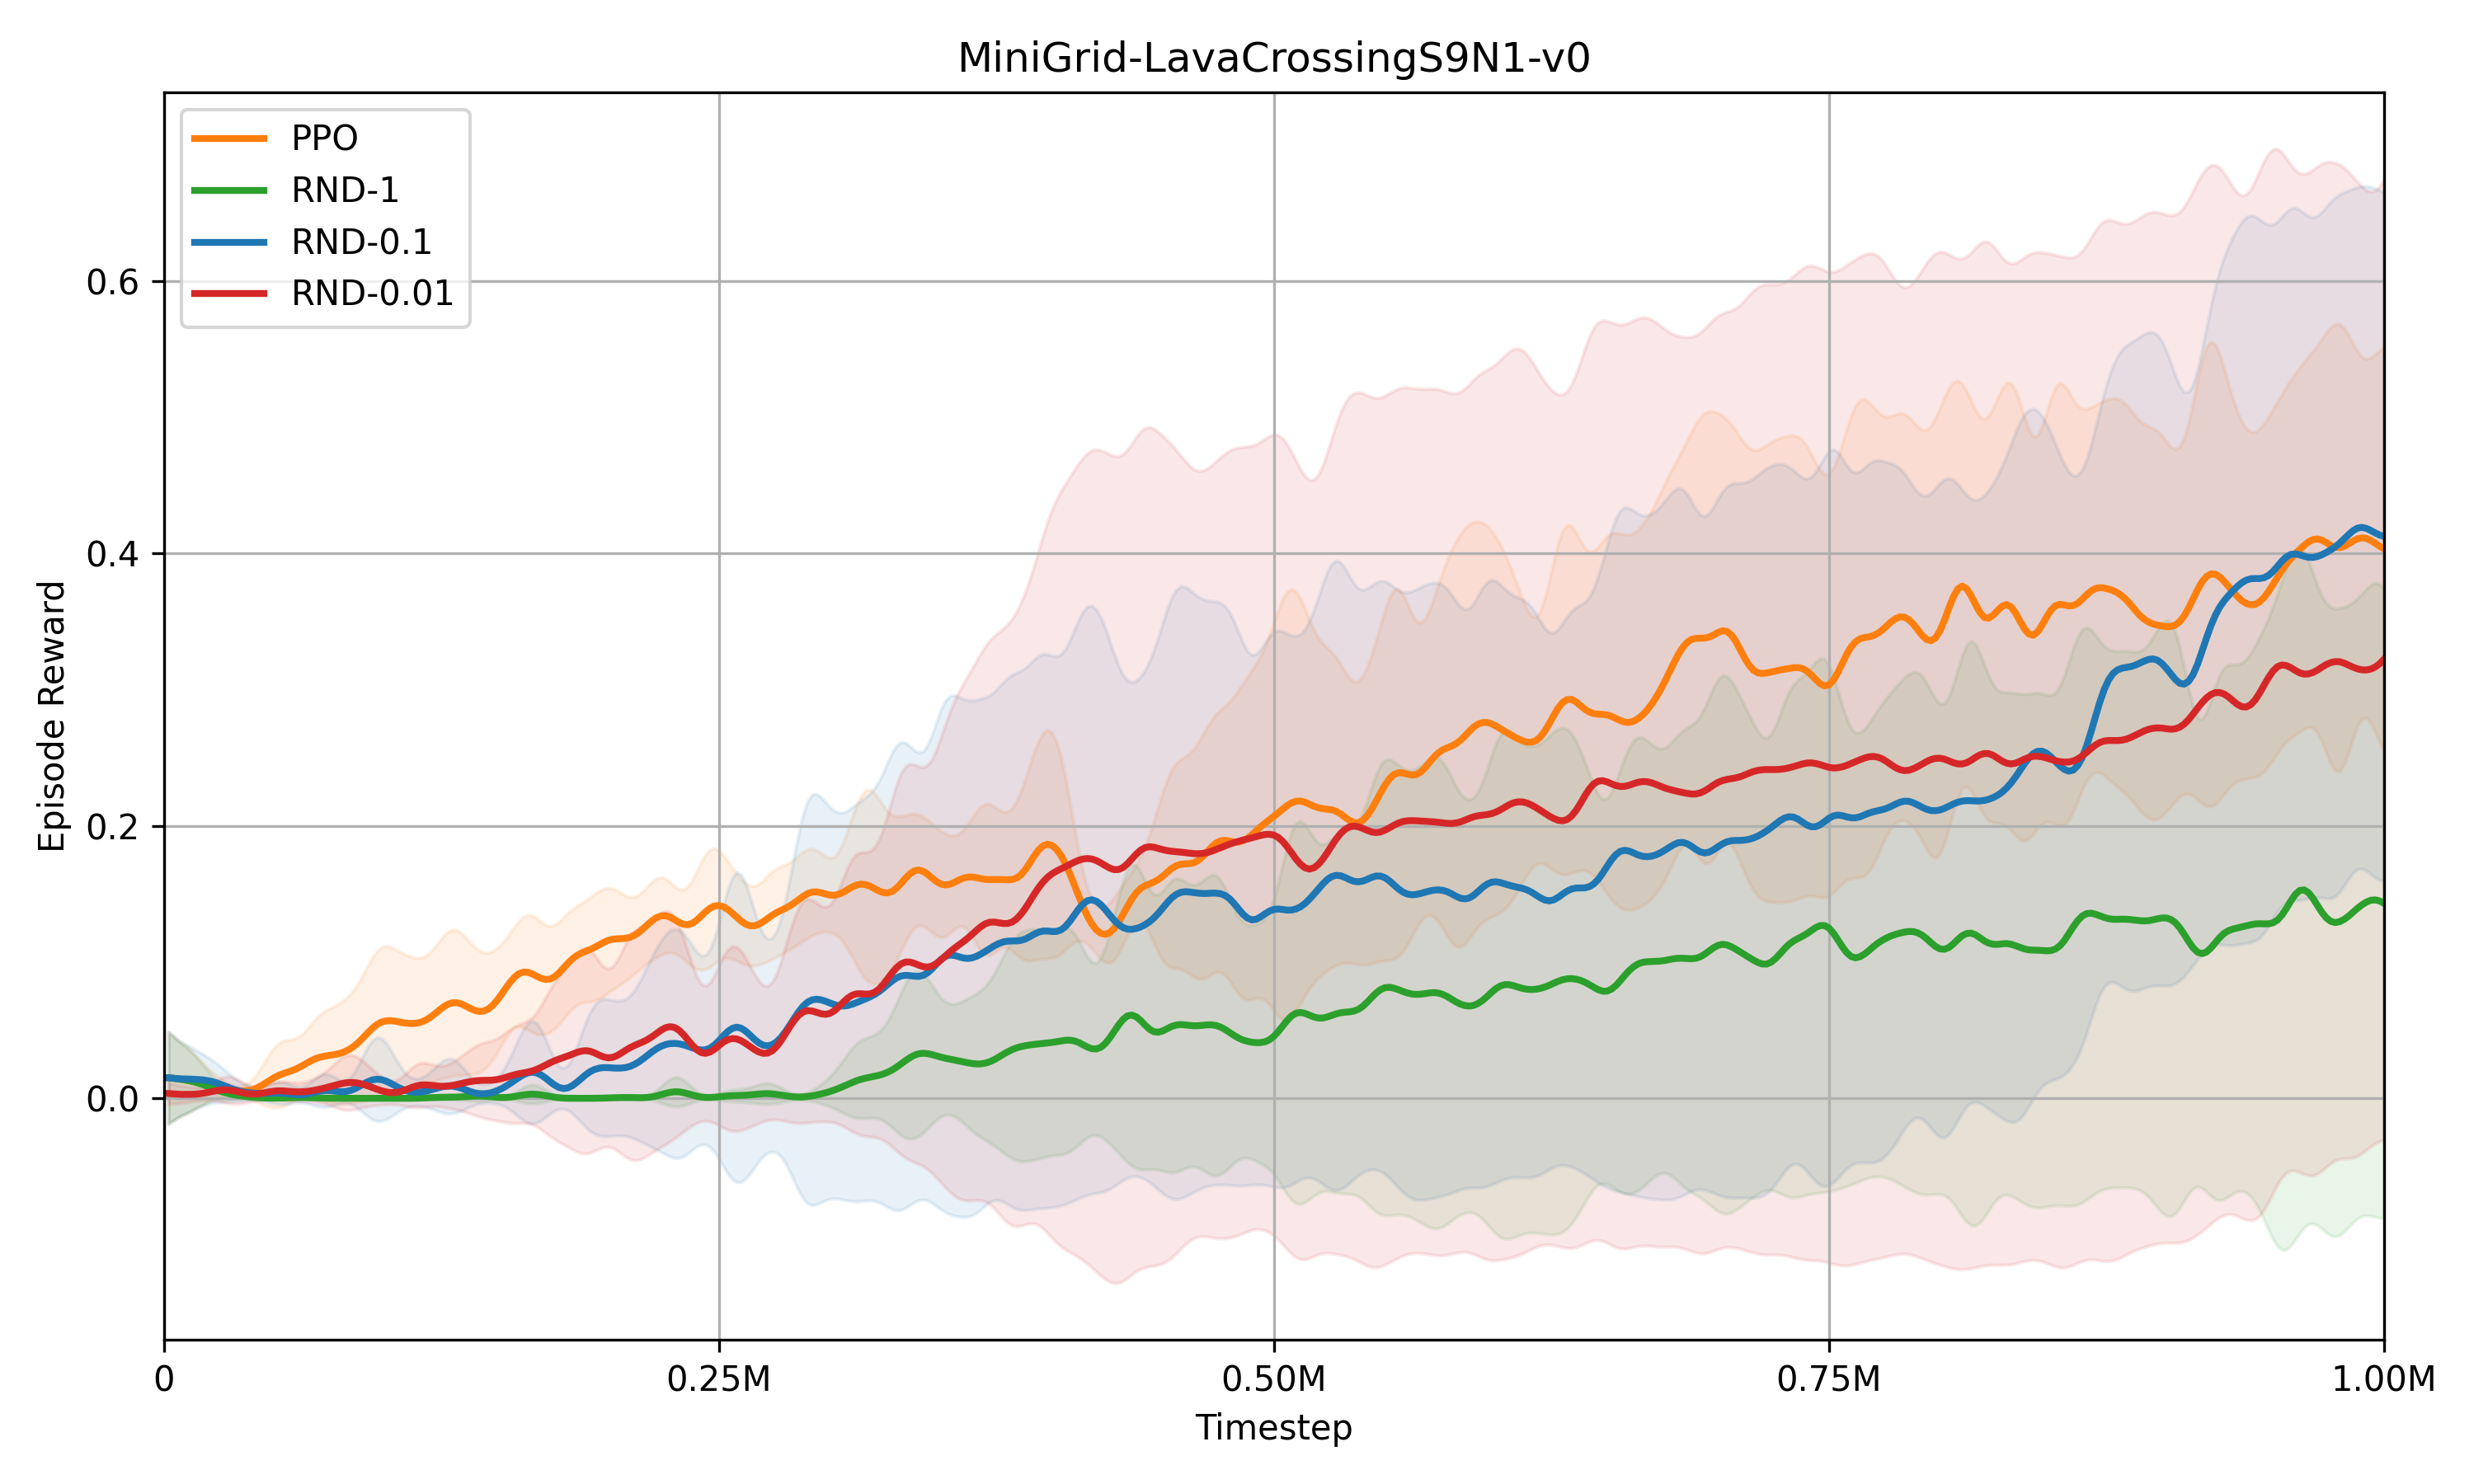
\includegraphics[width=\textwidth]{figs/MiniGrid-LavaCrossingS9N1-v0/episode_reward.png}
    
    (a) Episode Reward
\end{minipage}
\hfill
\begin{minipage}{0.45\textwidth}
    \centering
    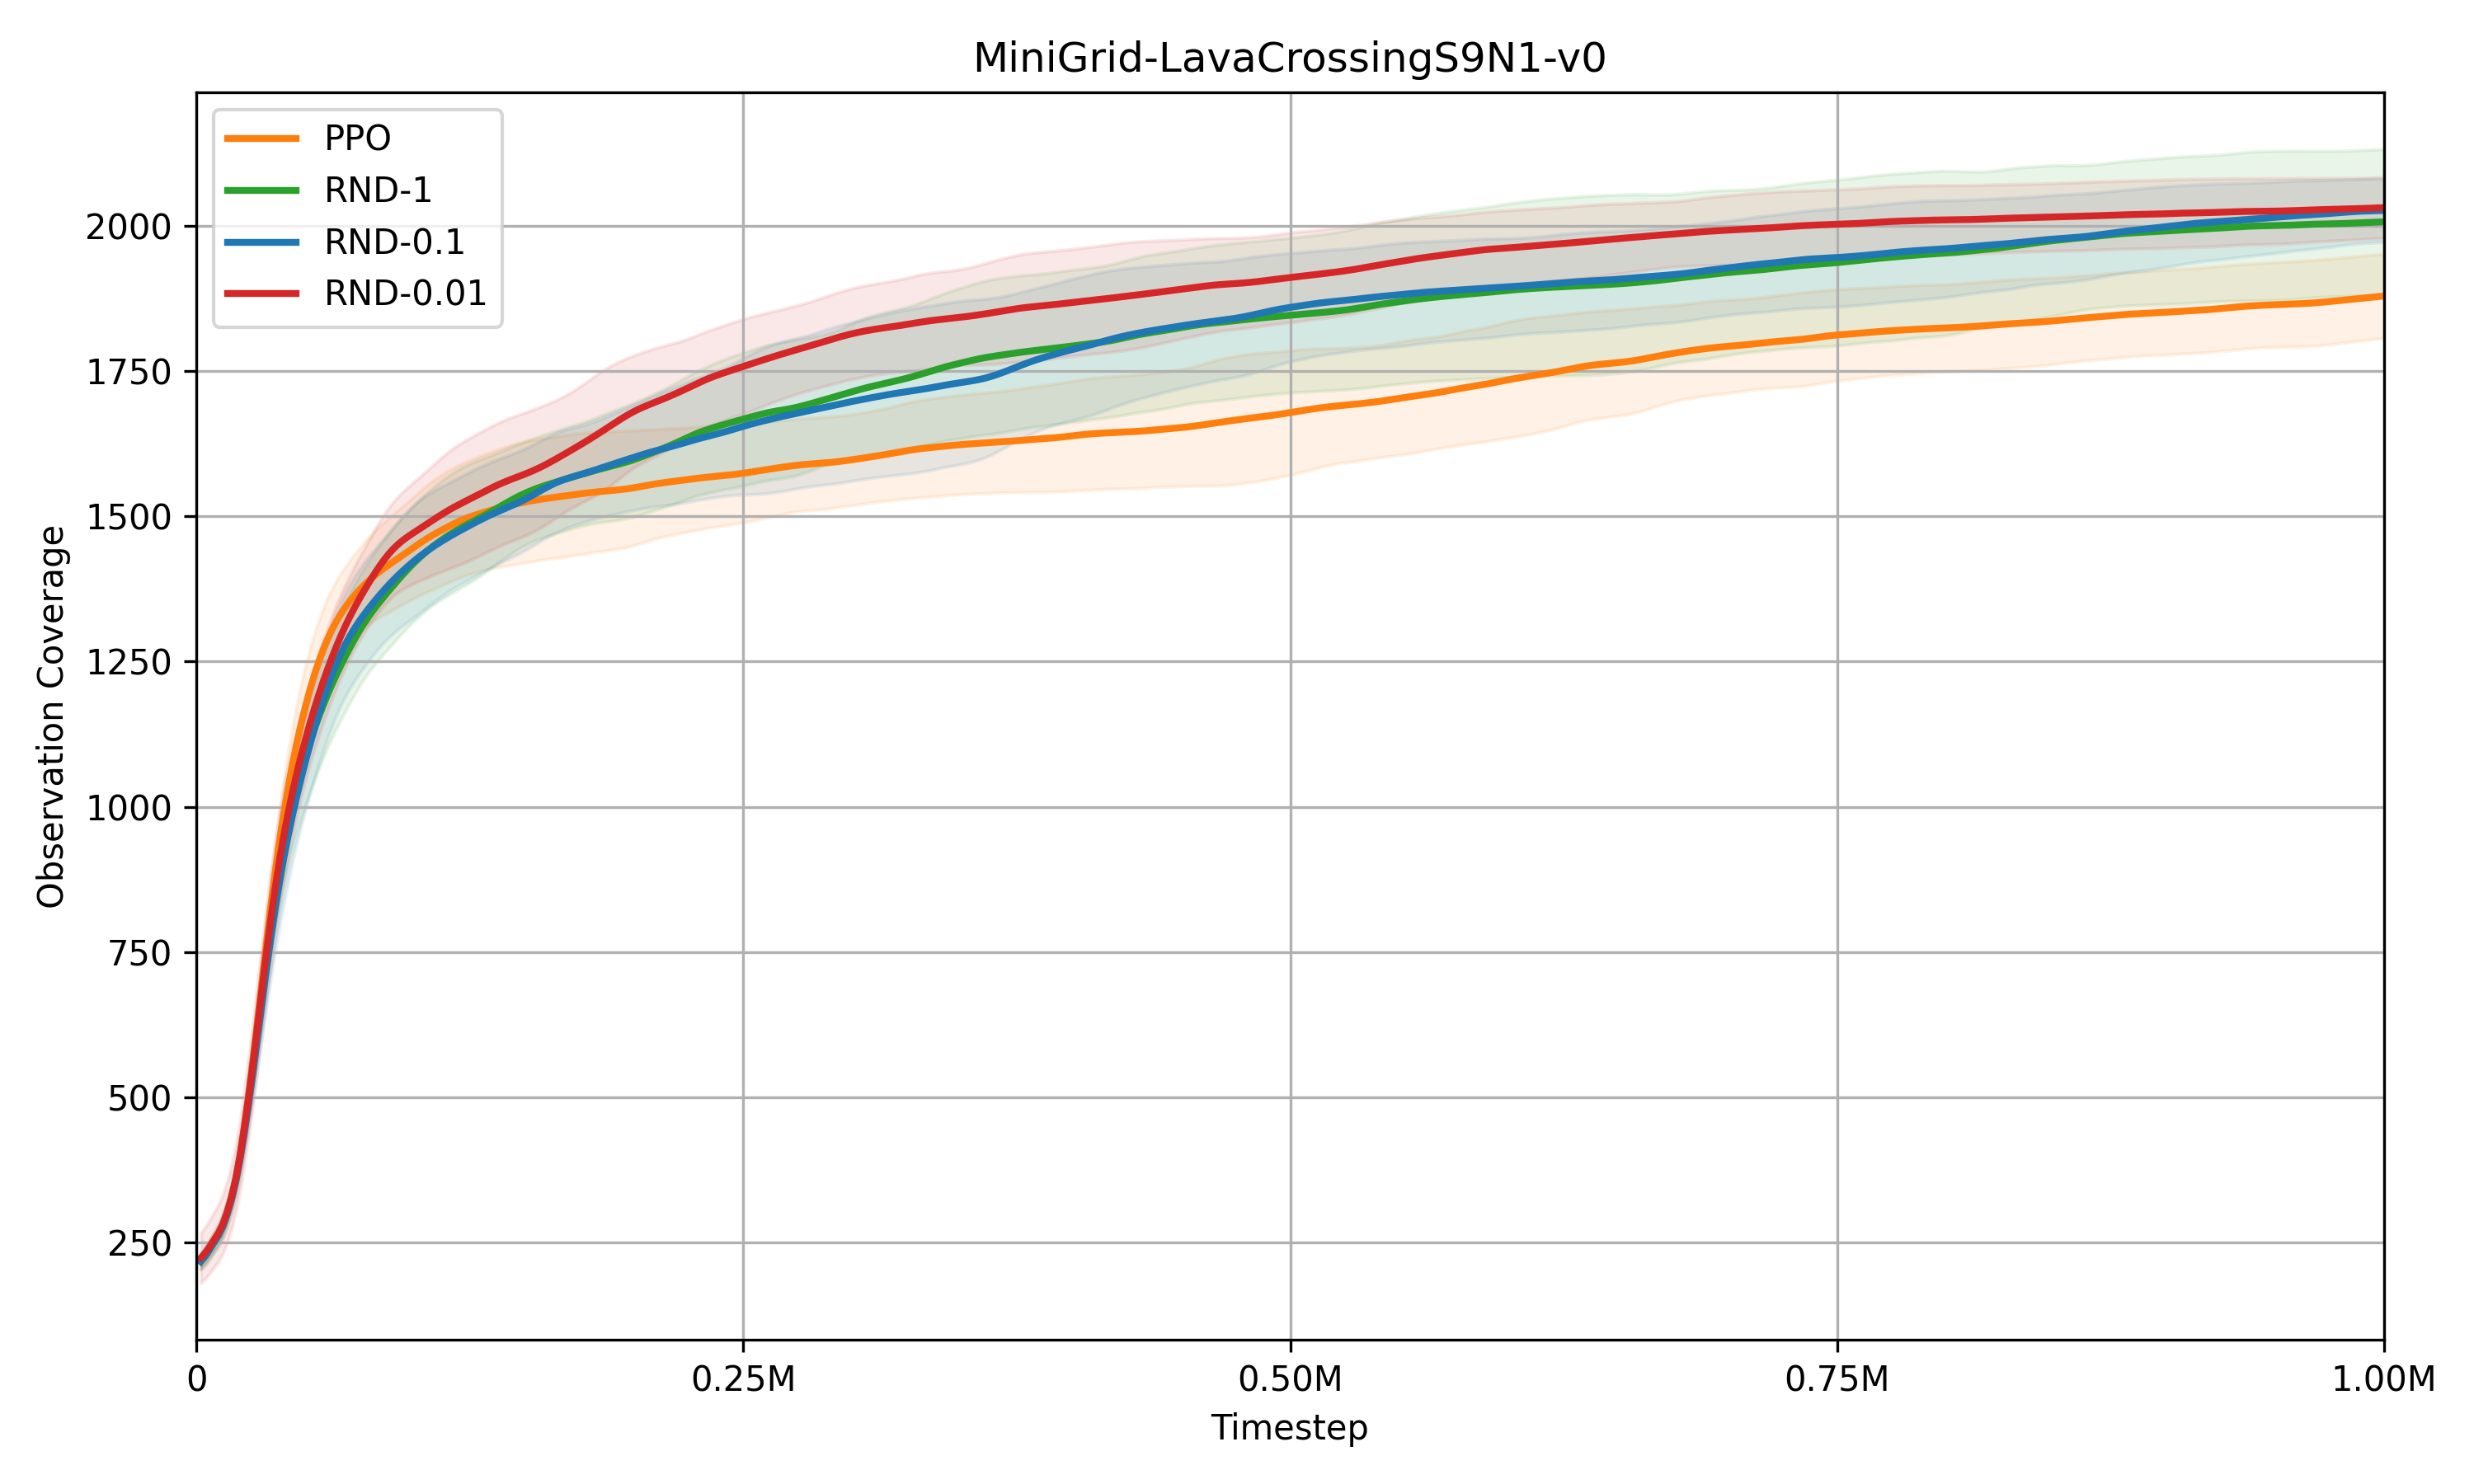
\includegraphics[width=\textwidth]{figs/MiniGrid-LavaCrossingS9N1-v0/obs_coverage.png}
    
    (b) Observation Coverage
\end{minipage}

\vspace{0.3cm}

\begin{minipage}{0.45\textwidth}
    \centering
    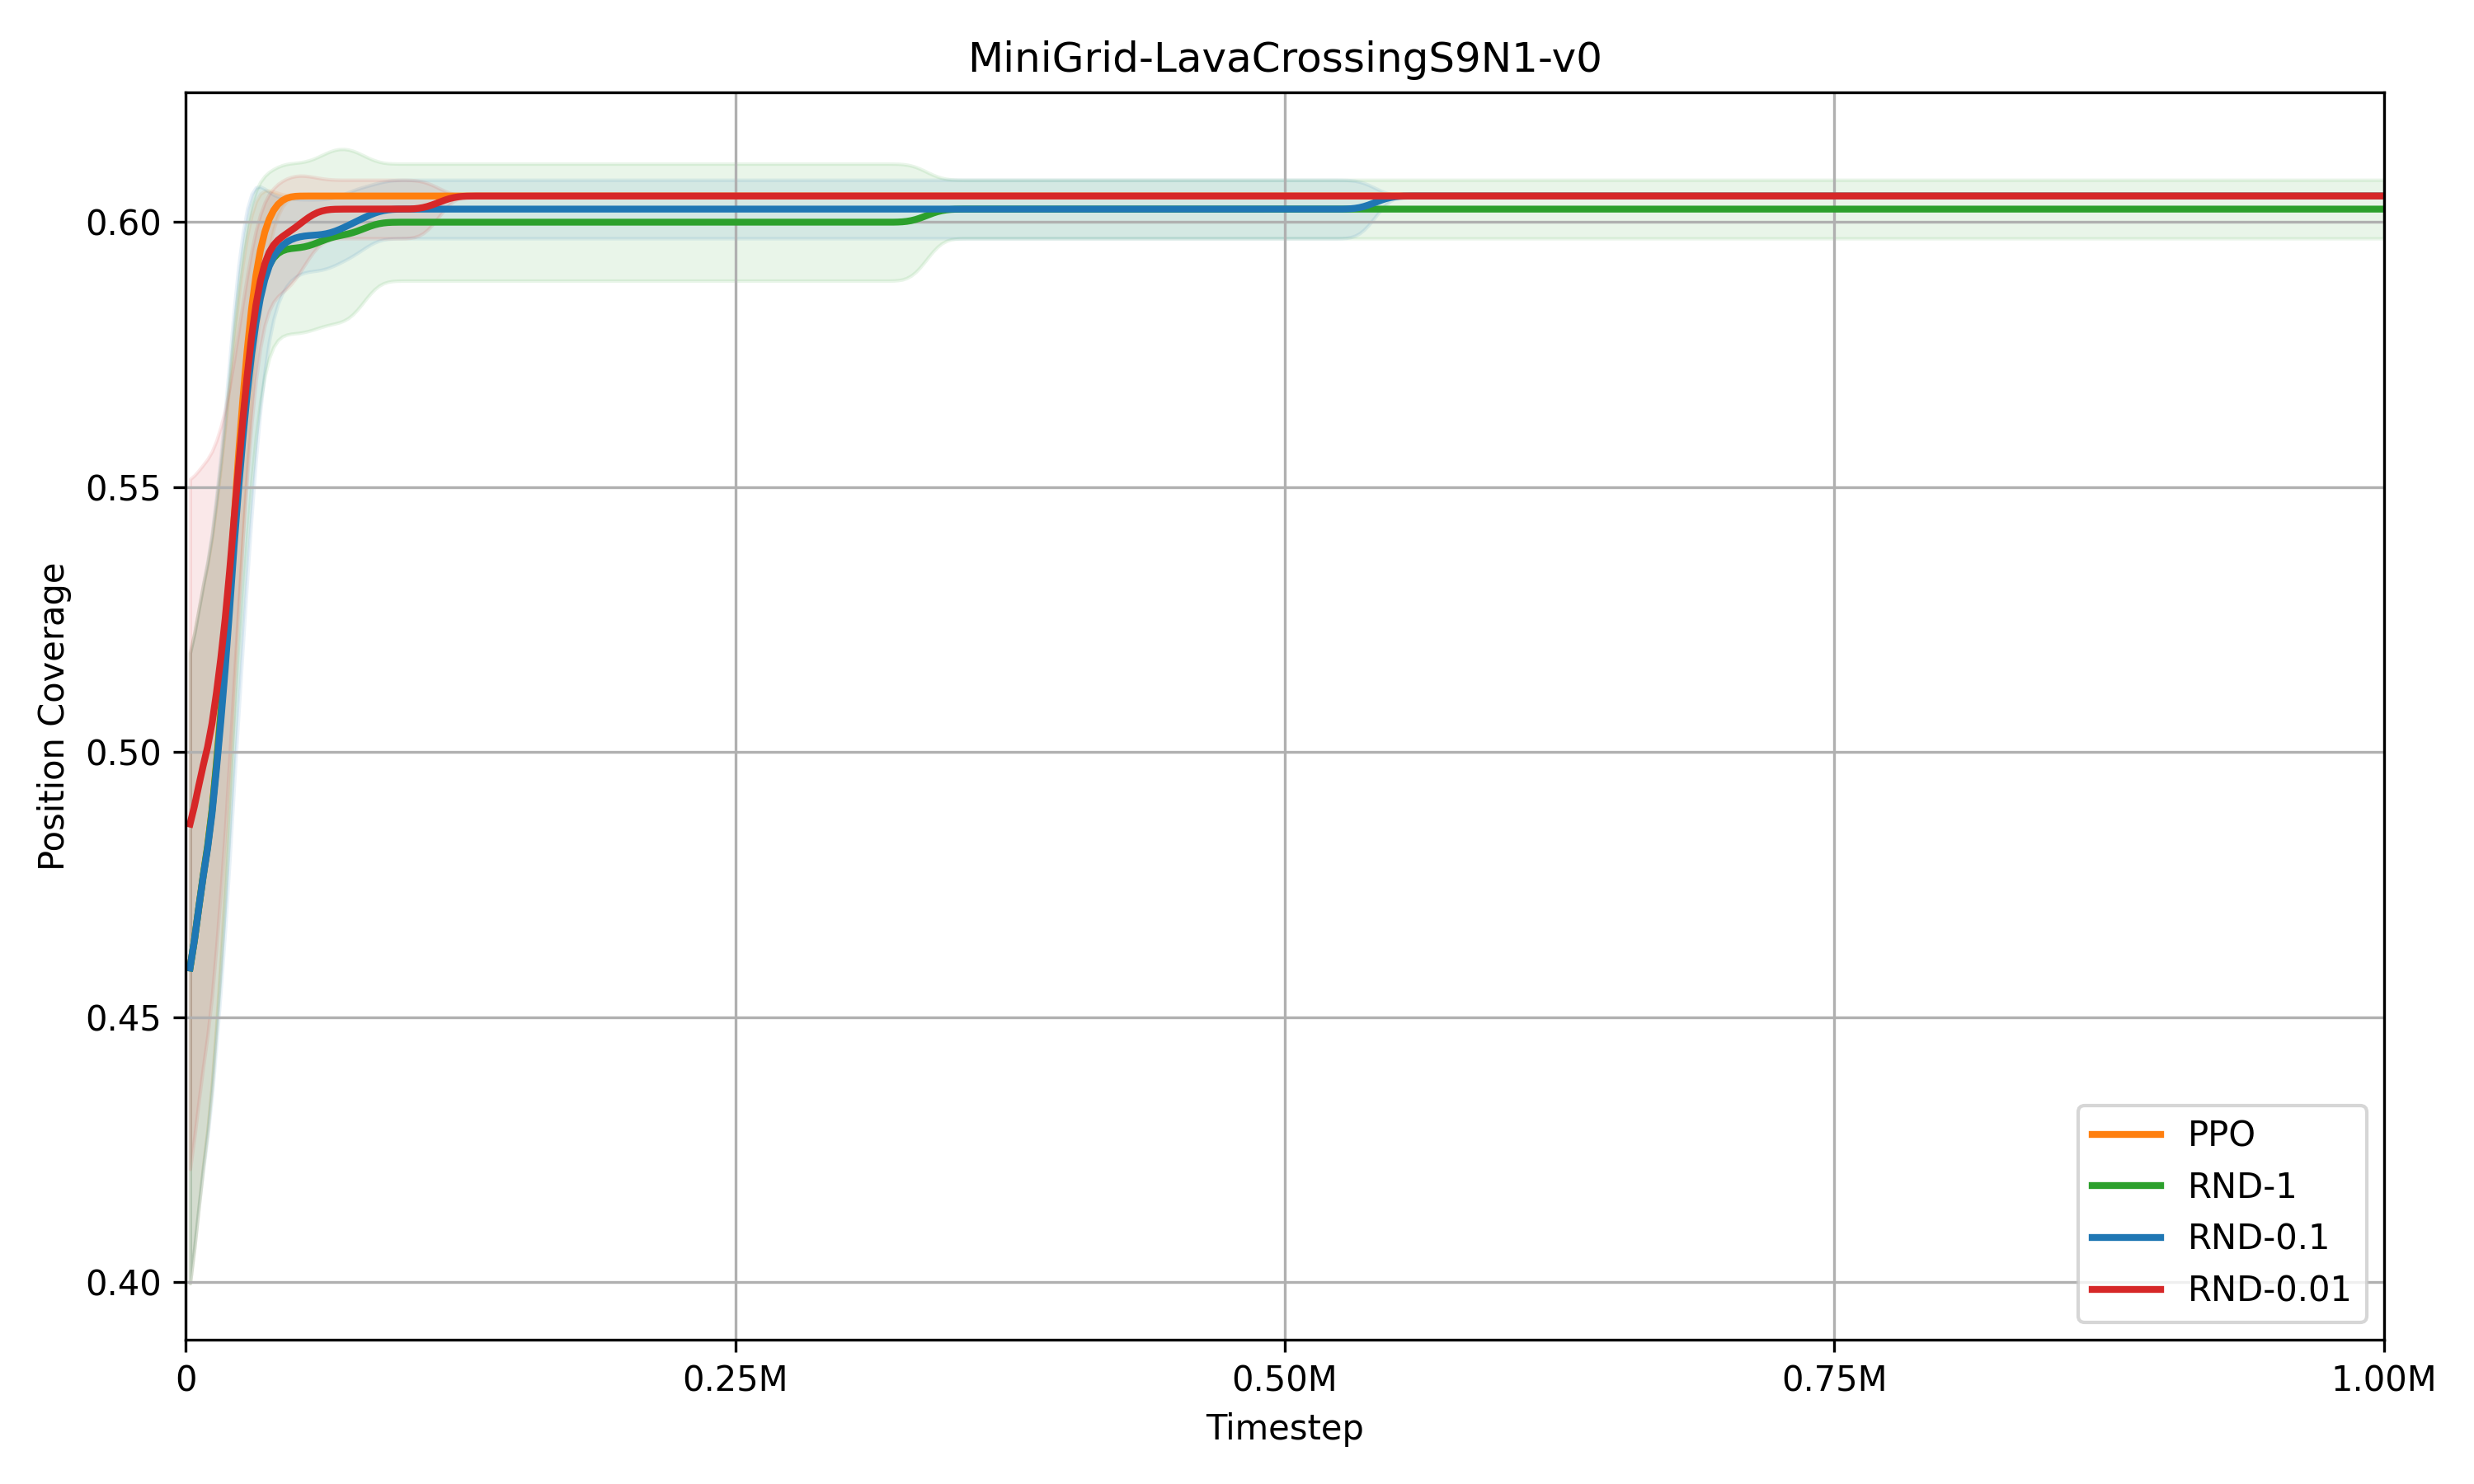
\includegraphics[width=\textwidth]{figs/MiniGrid-LavaCrossingS9N1-v0/pos_coverage.png}
    
    (c) Position Coverage
\end{minipage}
\hfill
\begin{minipage}{0.45\textwidth}
    \centering
    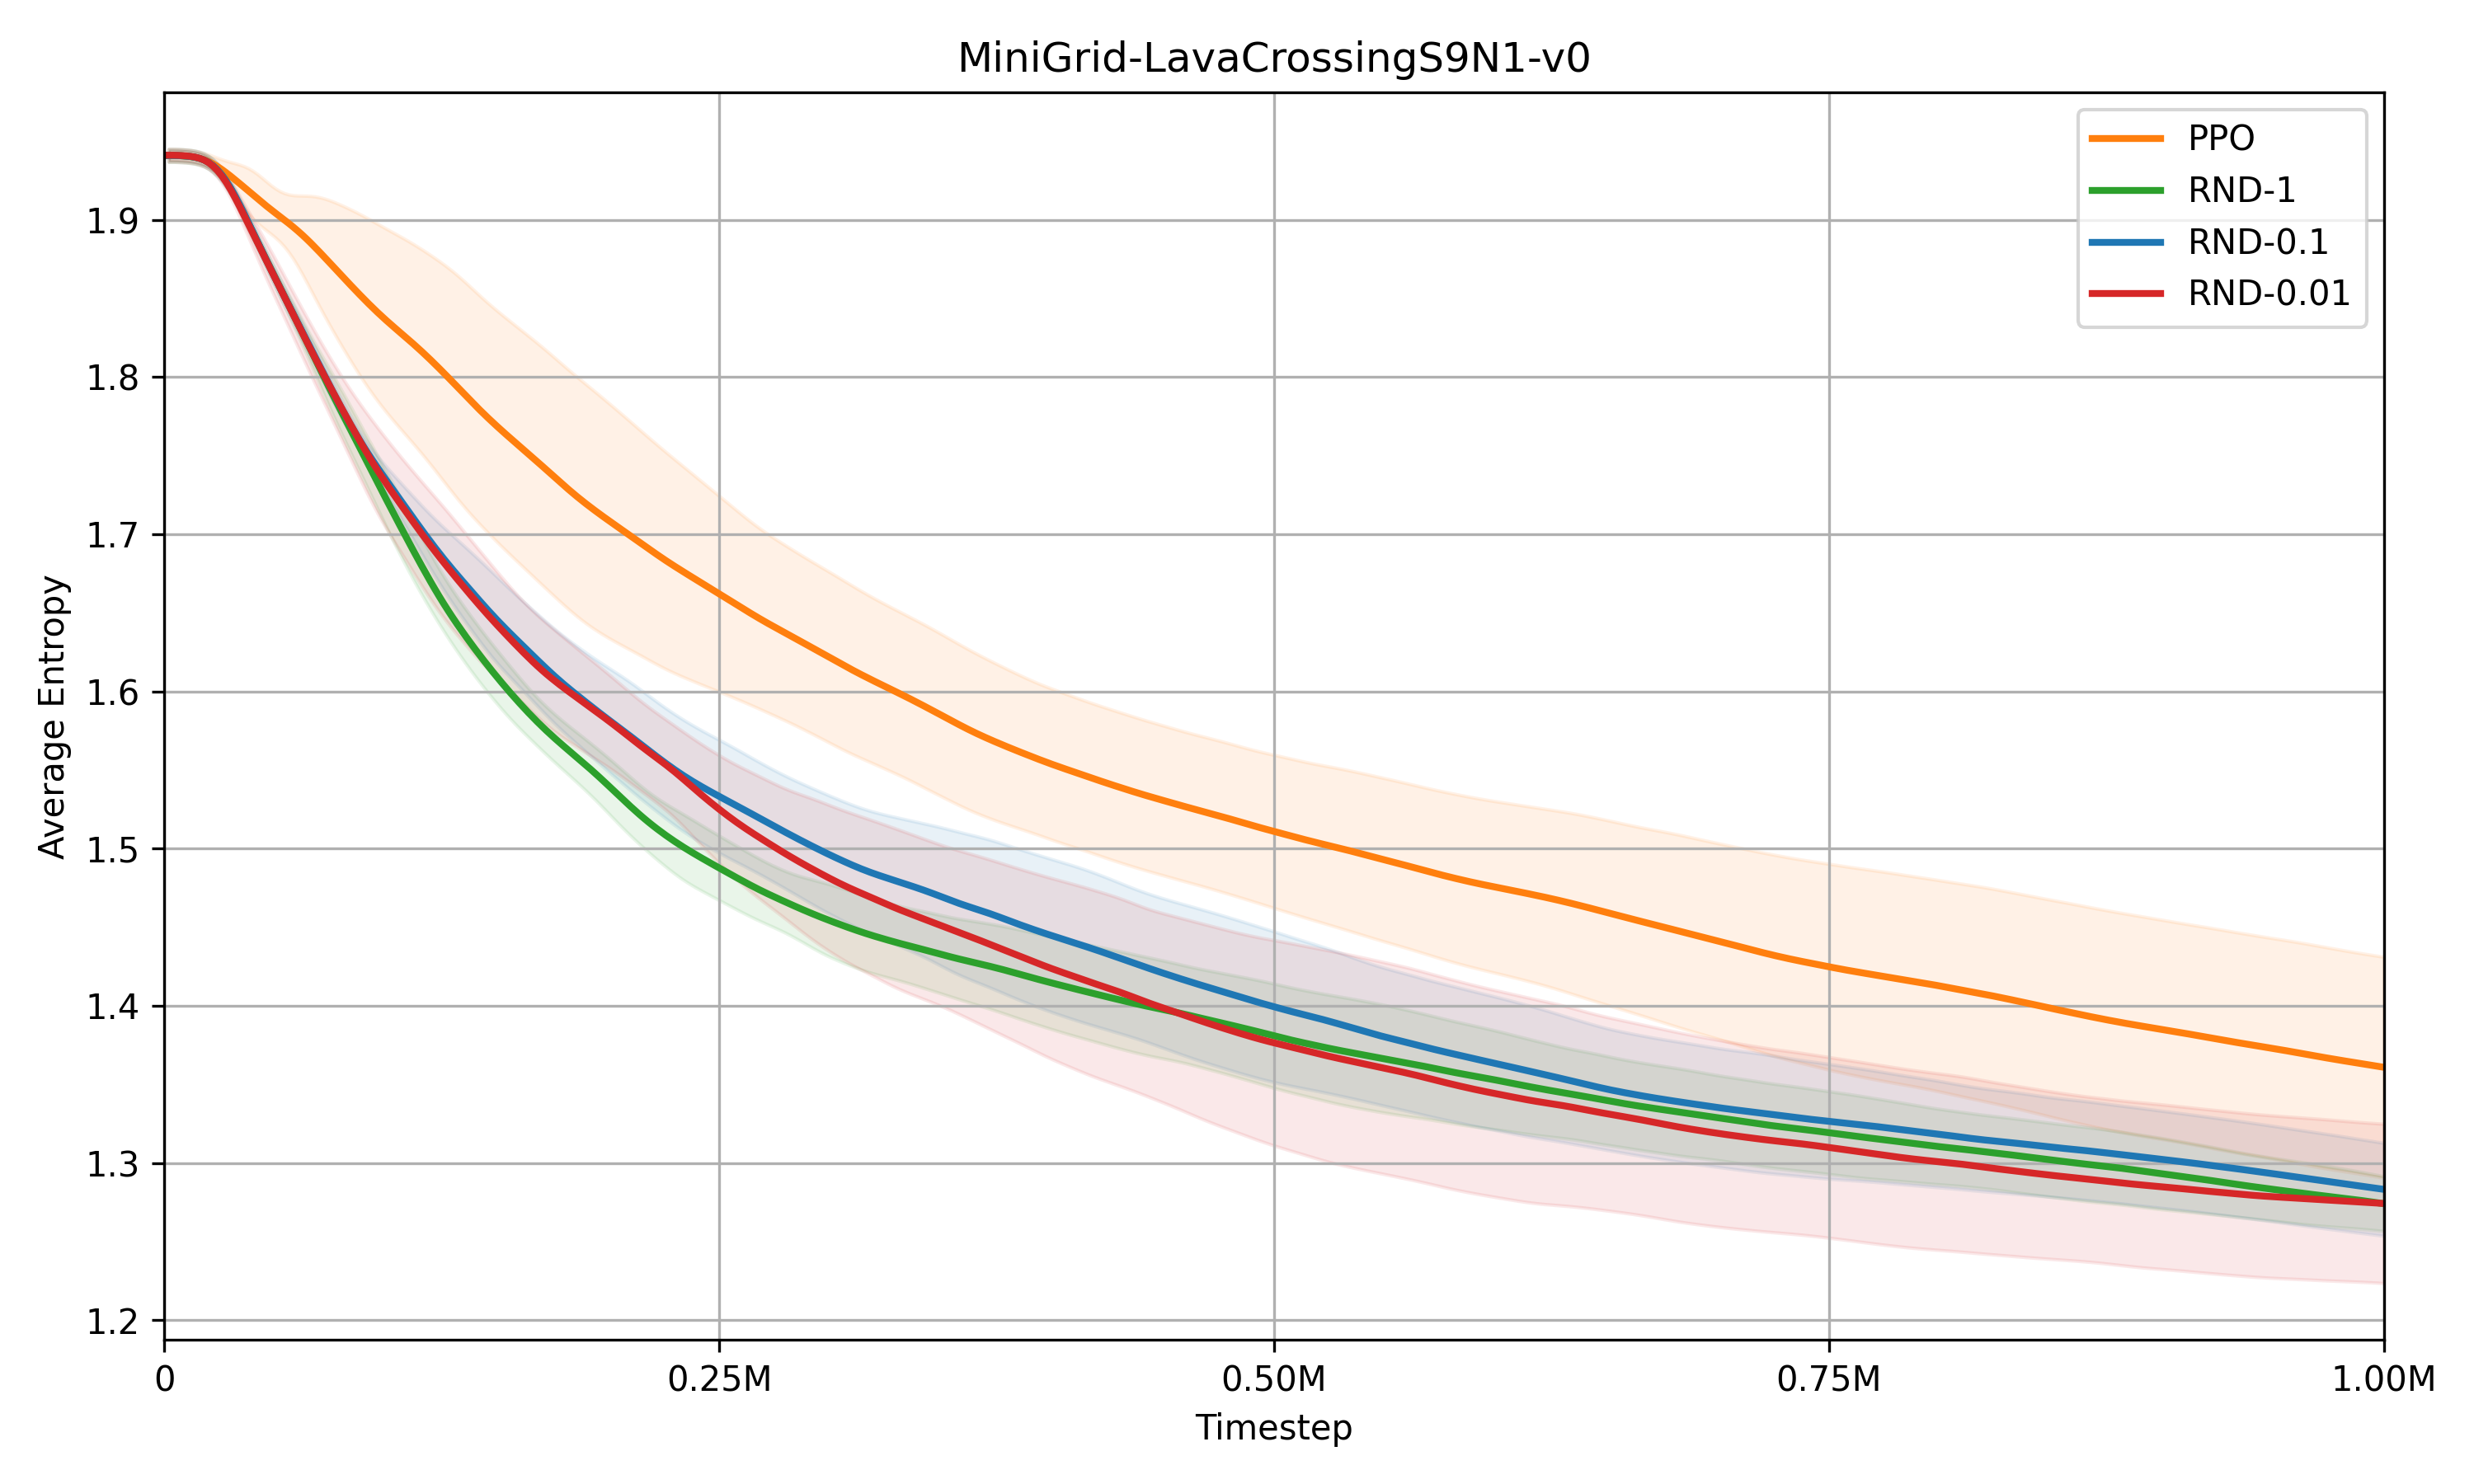
\includegraphics[width=\textwidth]{figs/MiniGrid-LavaCrossingS9N1-v0/avg_entropy.png}
    
    (d) Policy Entropy
\end{minipage}
\end{figure}

\begin{figure}[H]{Các chỉ số huấn luyện trên LavaCrossing-S9N2}
\centering
\begin{minipage}{0.45\textwidth}
    \centering
    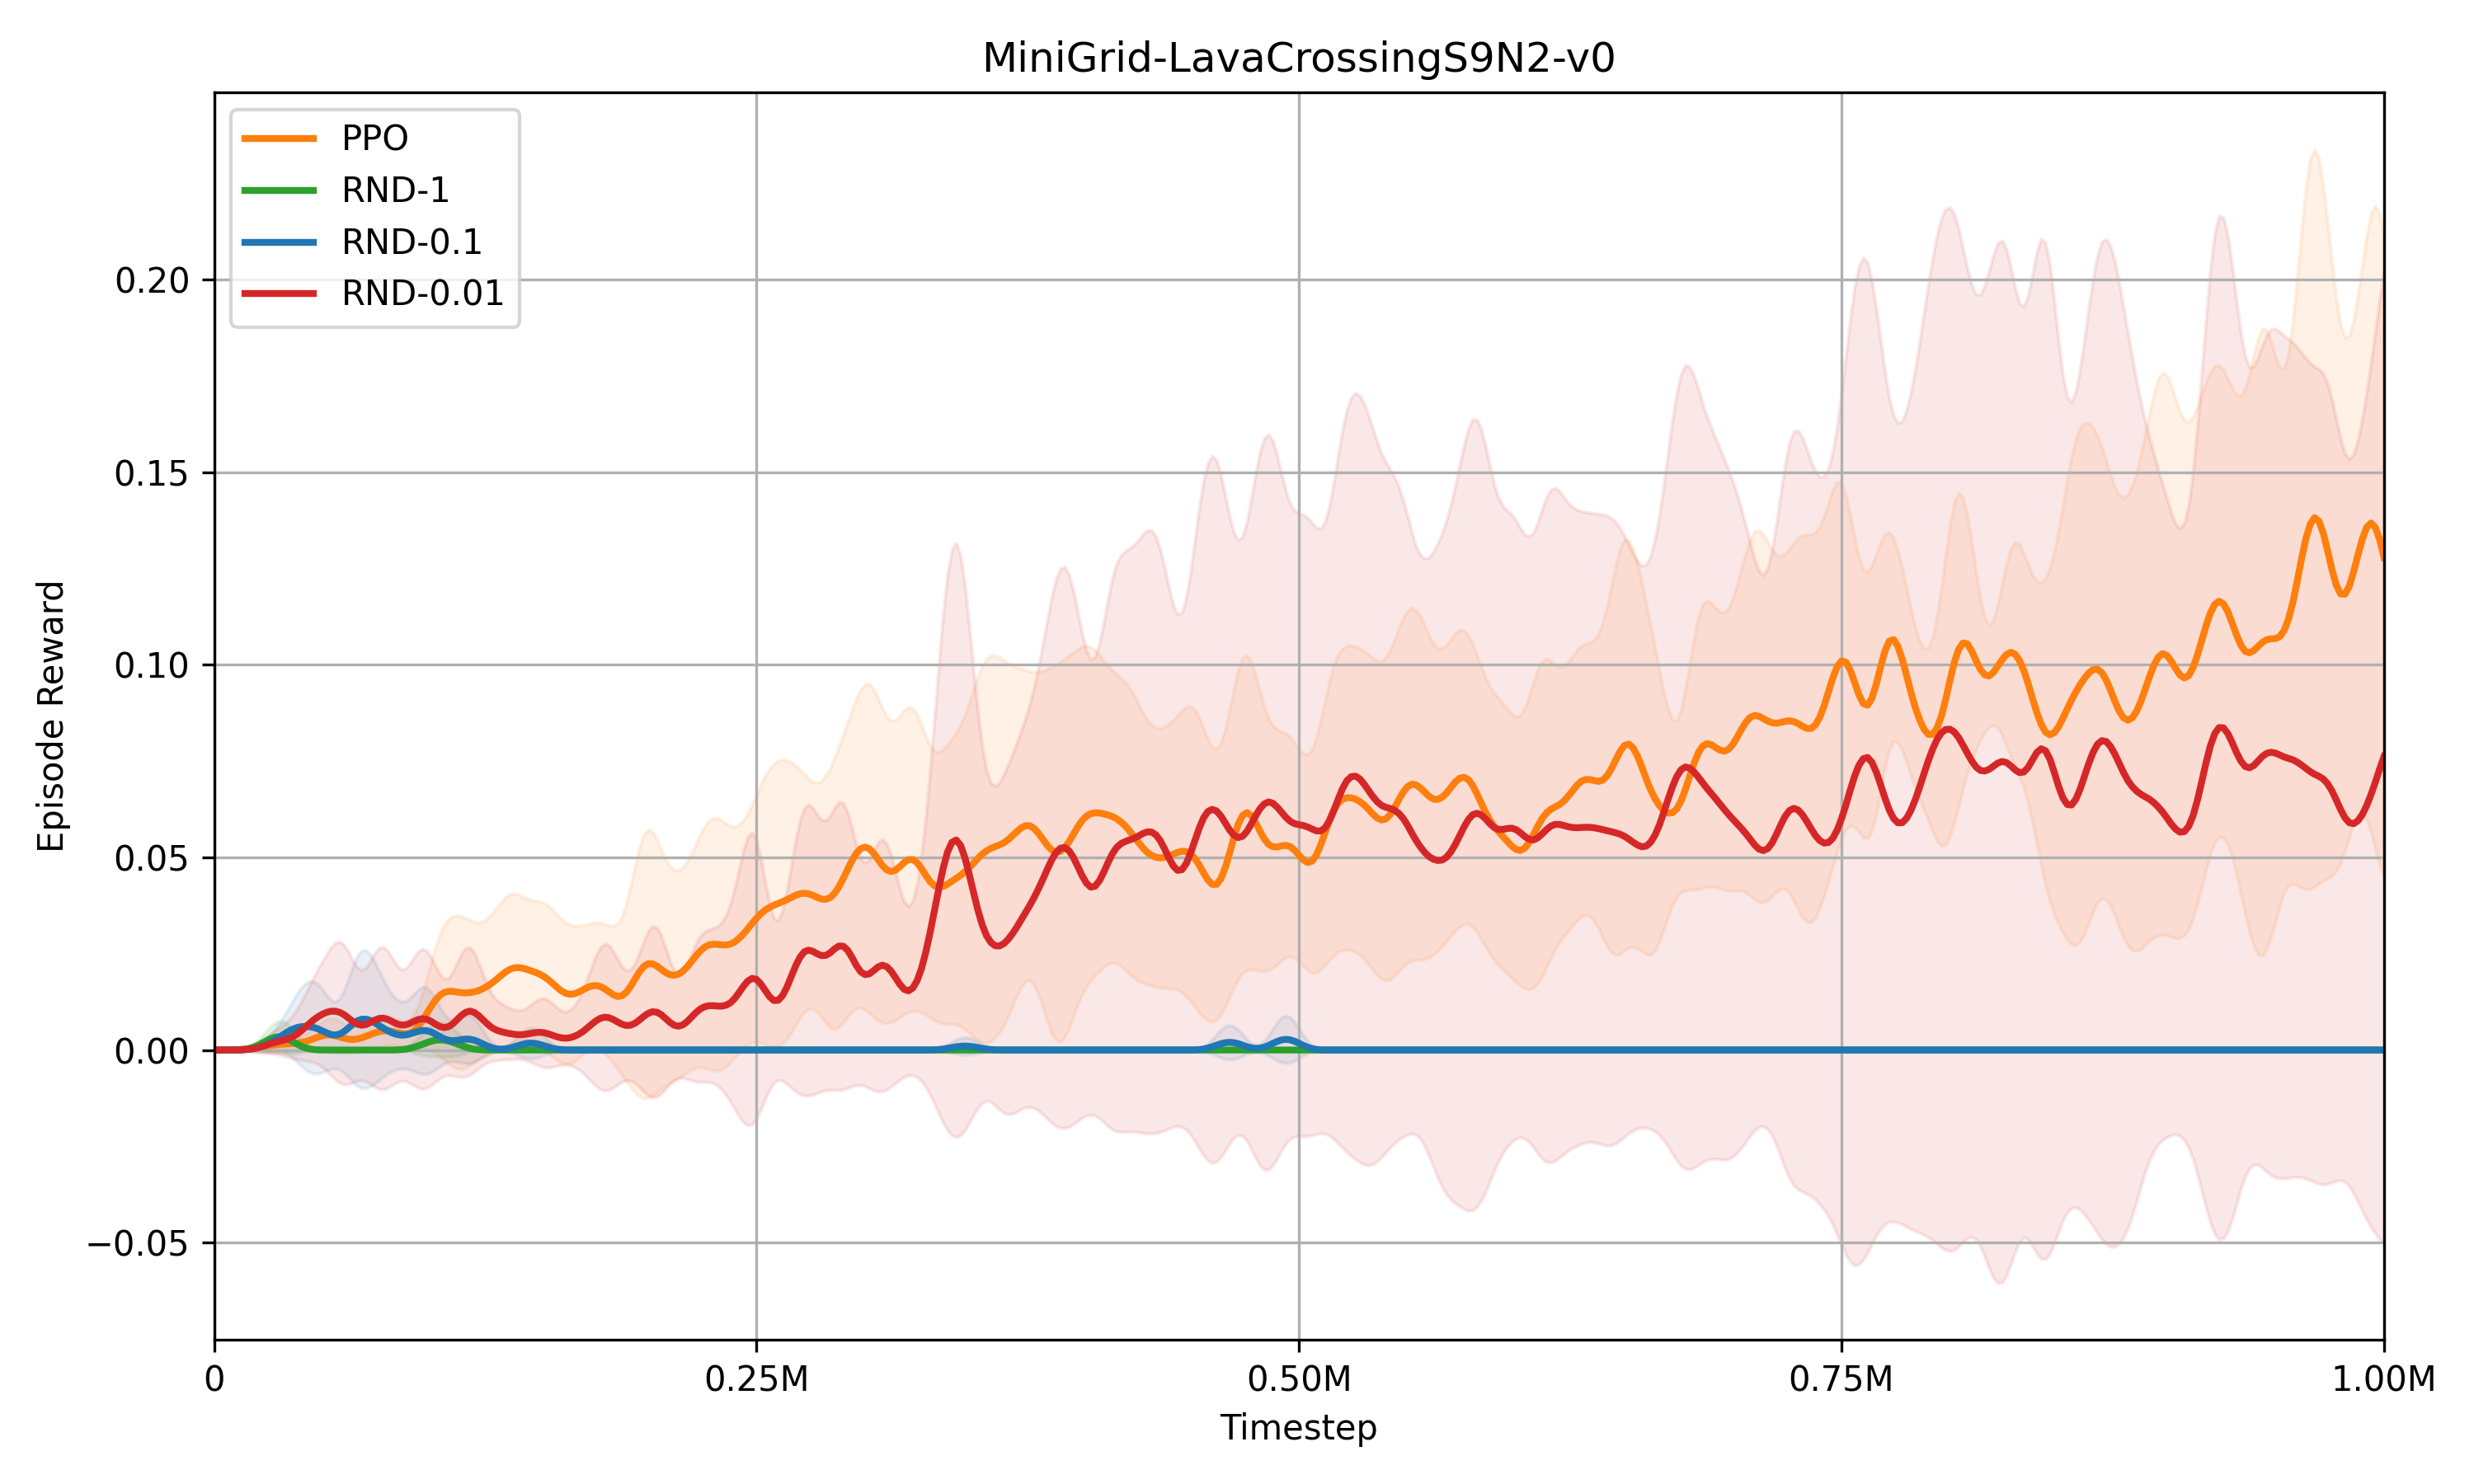
\includegraphics[width=\textwidth]{figs/MiniGrid-LavaCrossingS9N2-v0/episode_reward.png}
    
    (a) Episode Reward
\end{minipage}
\hfill
\begin{minipage}{0.45\textwidth}
    \centering
    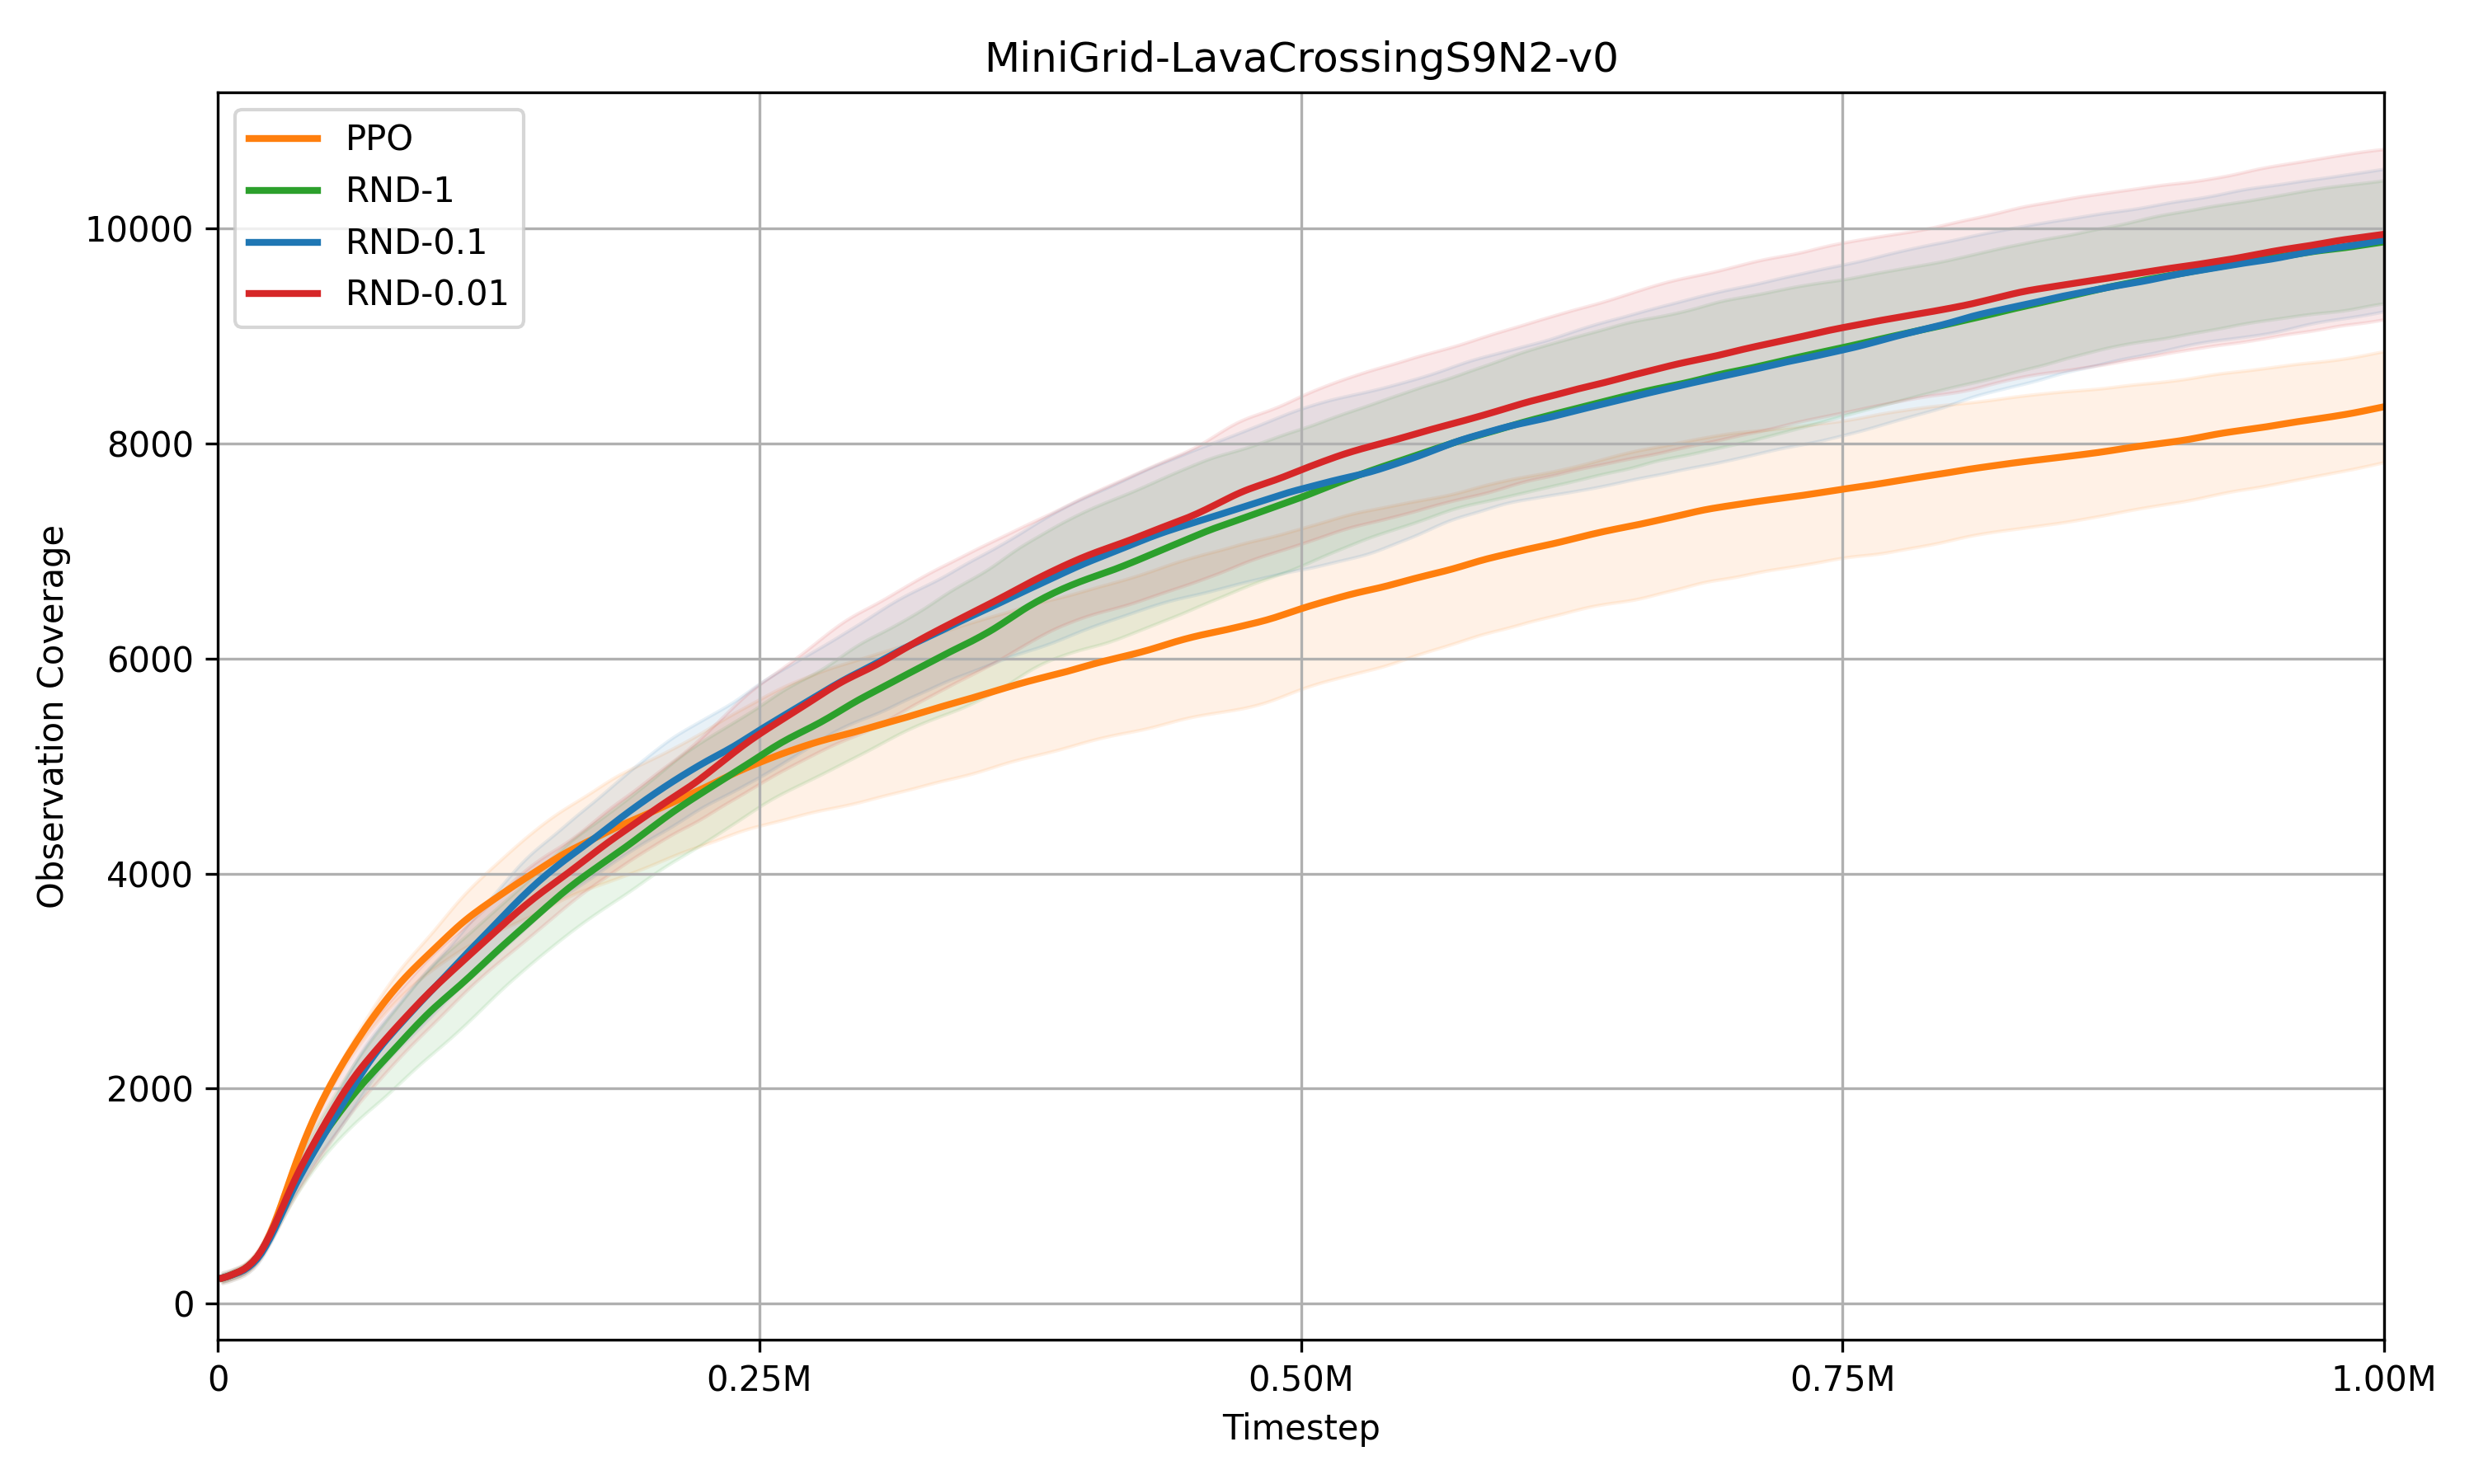
\includegraphics[width=\textwidth]{figs/MiniGrid-LavaCrossingS9N2-v0/obs_coverage.png}
    
    (b) Observation Coverage
\end{minipage}

\vspace{0.3cm}

\begin{minipage}{0.45\textwidth}
    \centering
    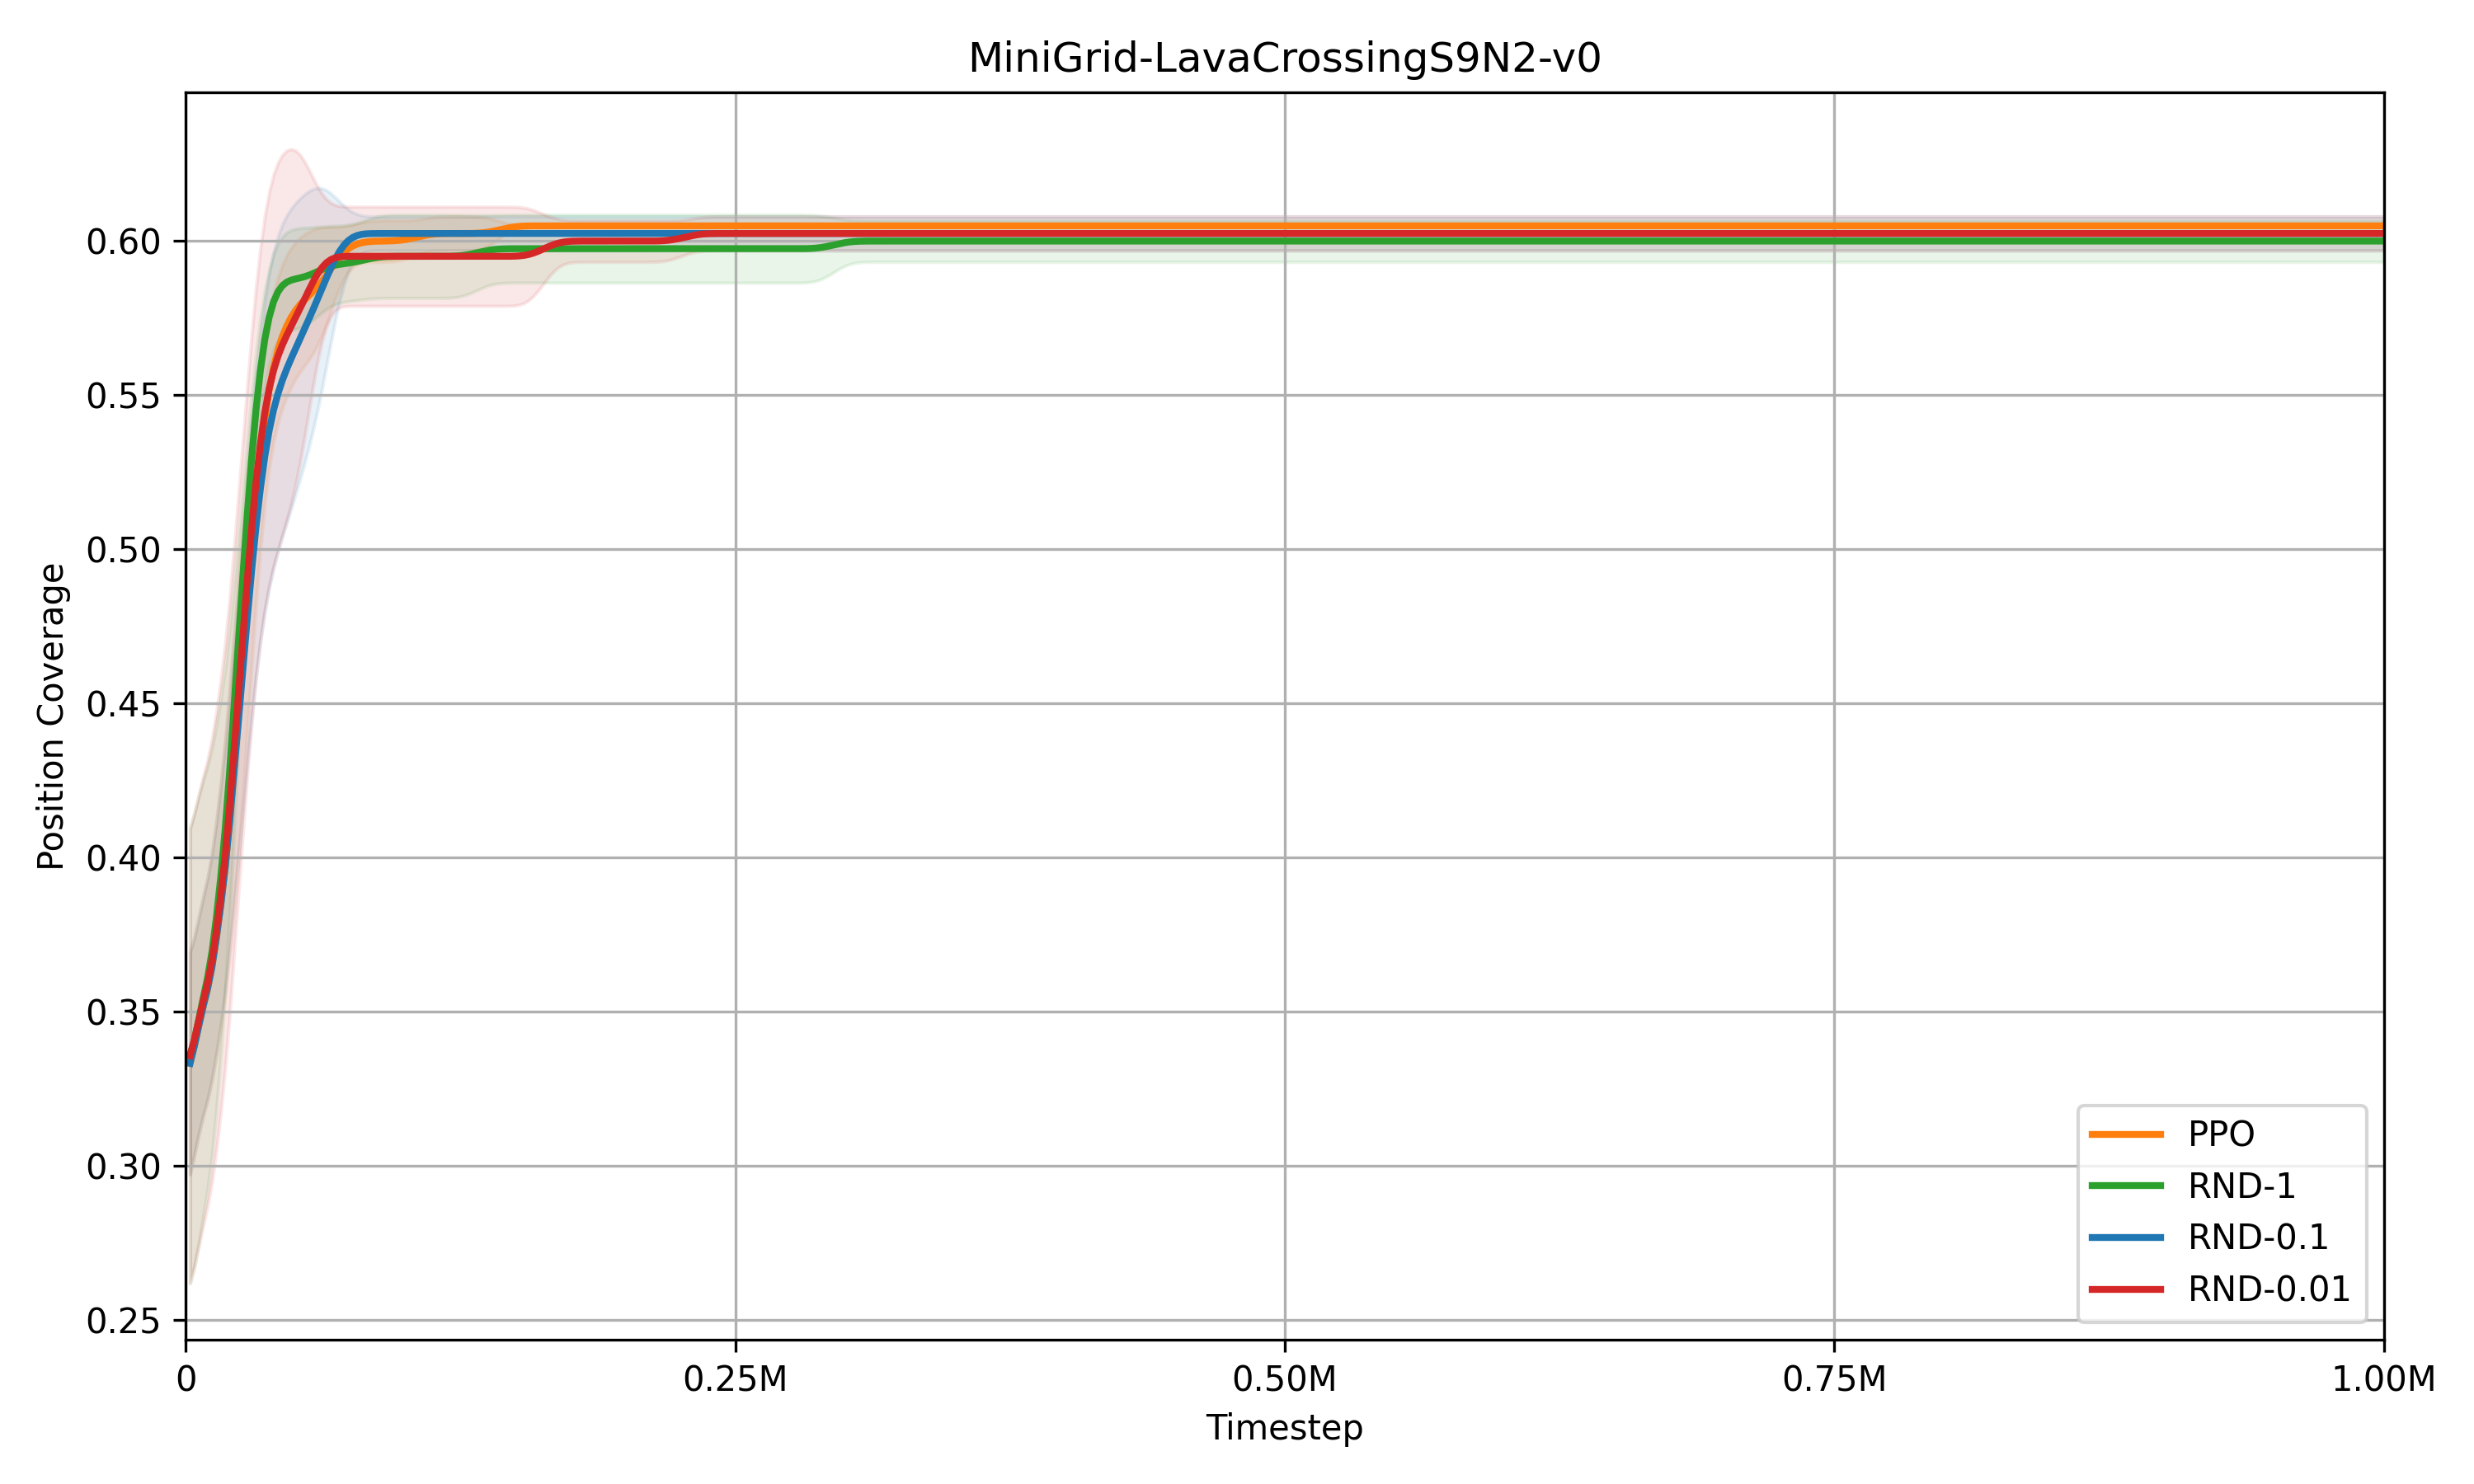
\includegraphics[width=\textwidth]{figs/MiniGrid-LavaCrossingS9N2-v0/pos_coverage.png}
    
    (c) Position Coverage
\end{minipage}
\hfill
\begin{minipage}{0.45\textwidth}
    \centering
    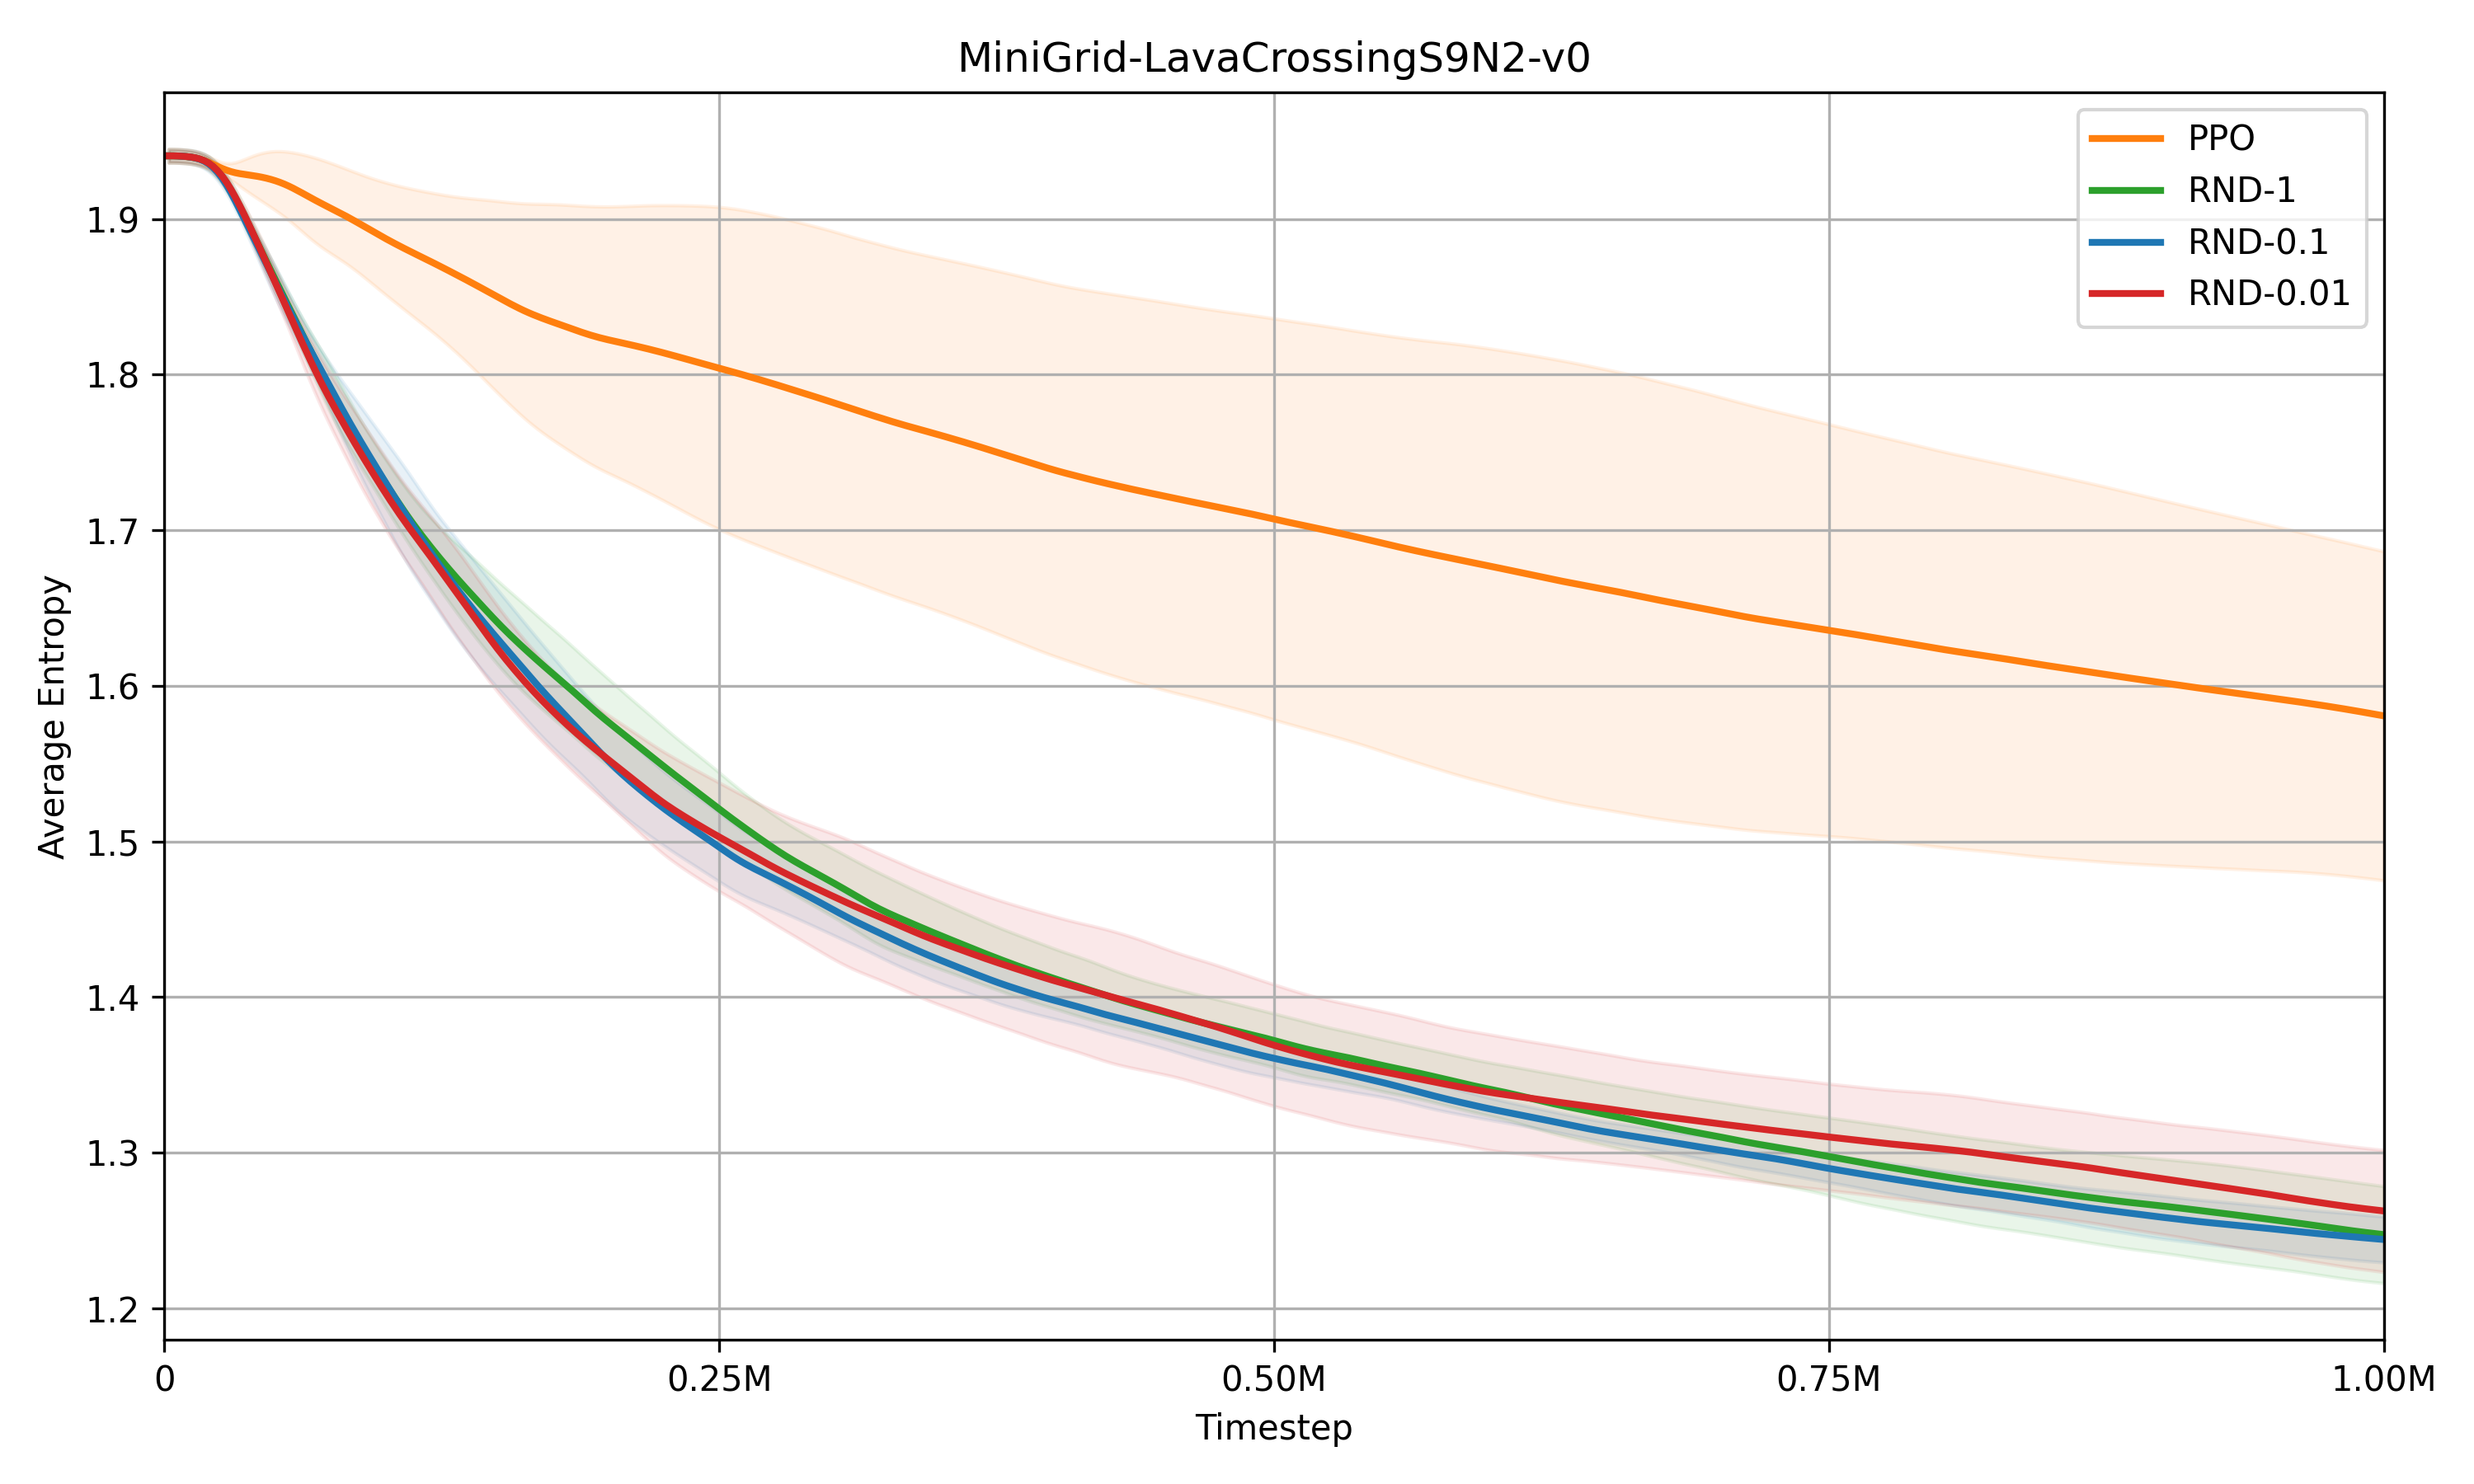
\includegraphics[width=\textwidth]{figs/MiniGrid-LavaCrossingS9N2-v0/avg_entropy.png}
    
    (d) Policy Entropy
\end{minipage}
\end{figure}

\begin{figure}[H]{Các chỉ số huấn luyện trên LavaCrossing-S9N3}
\centering
\begin{minipage}{0.45\textwidth}
    \centering
    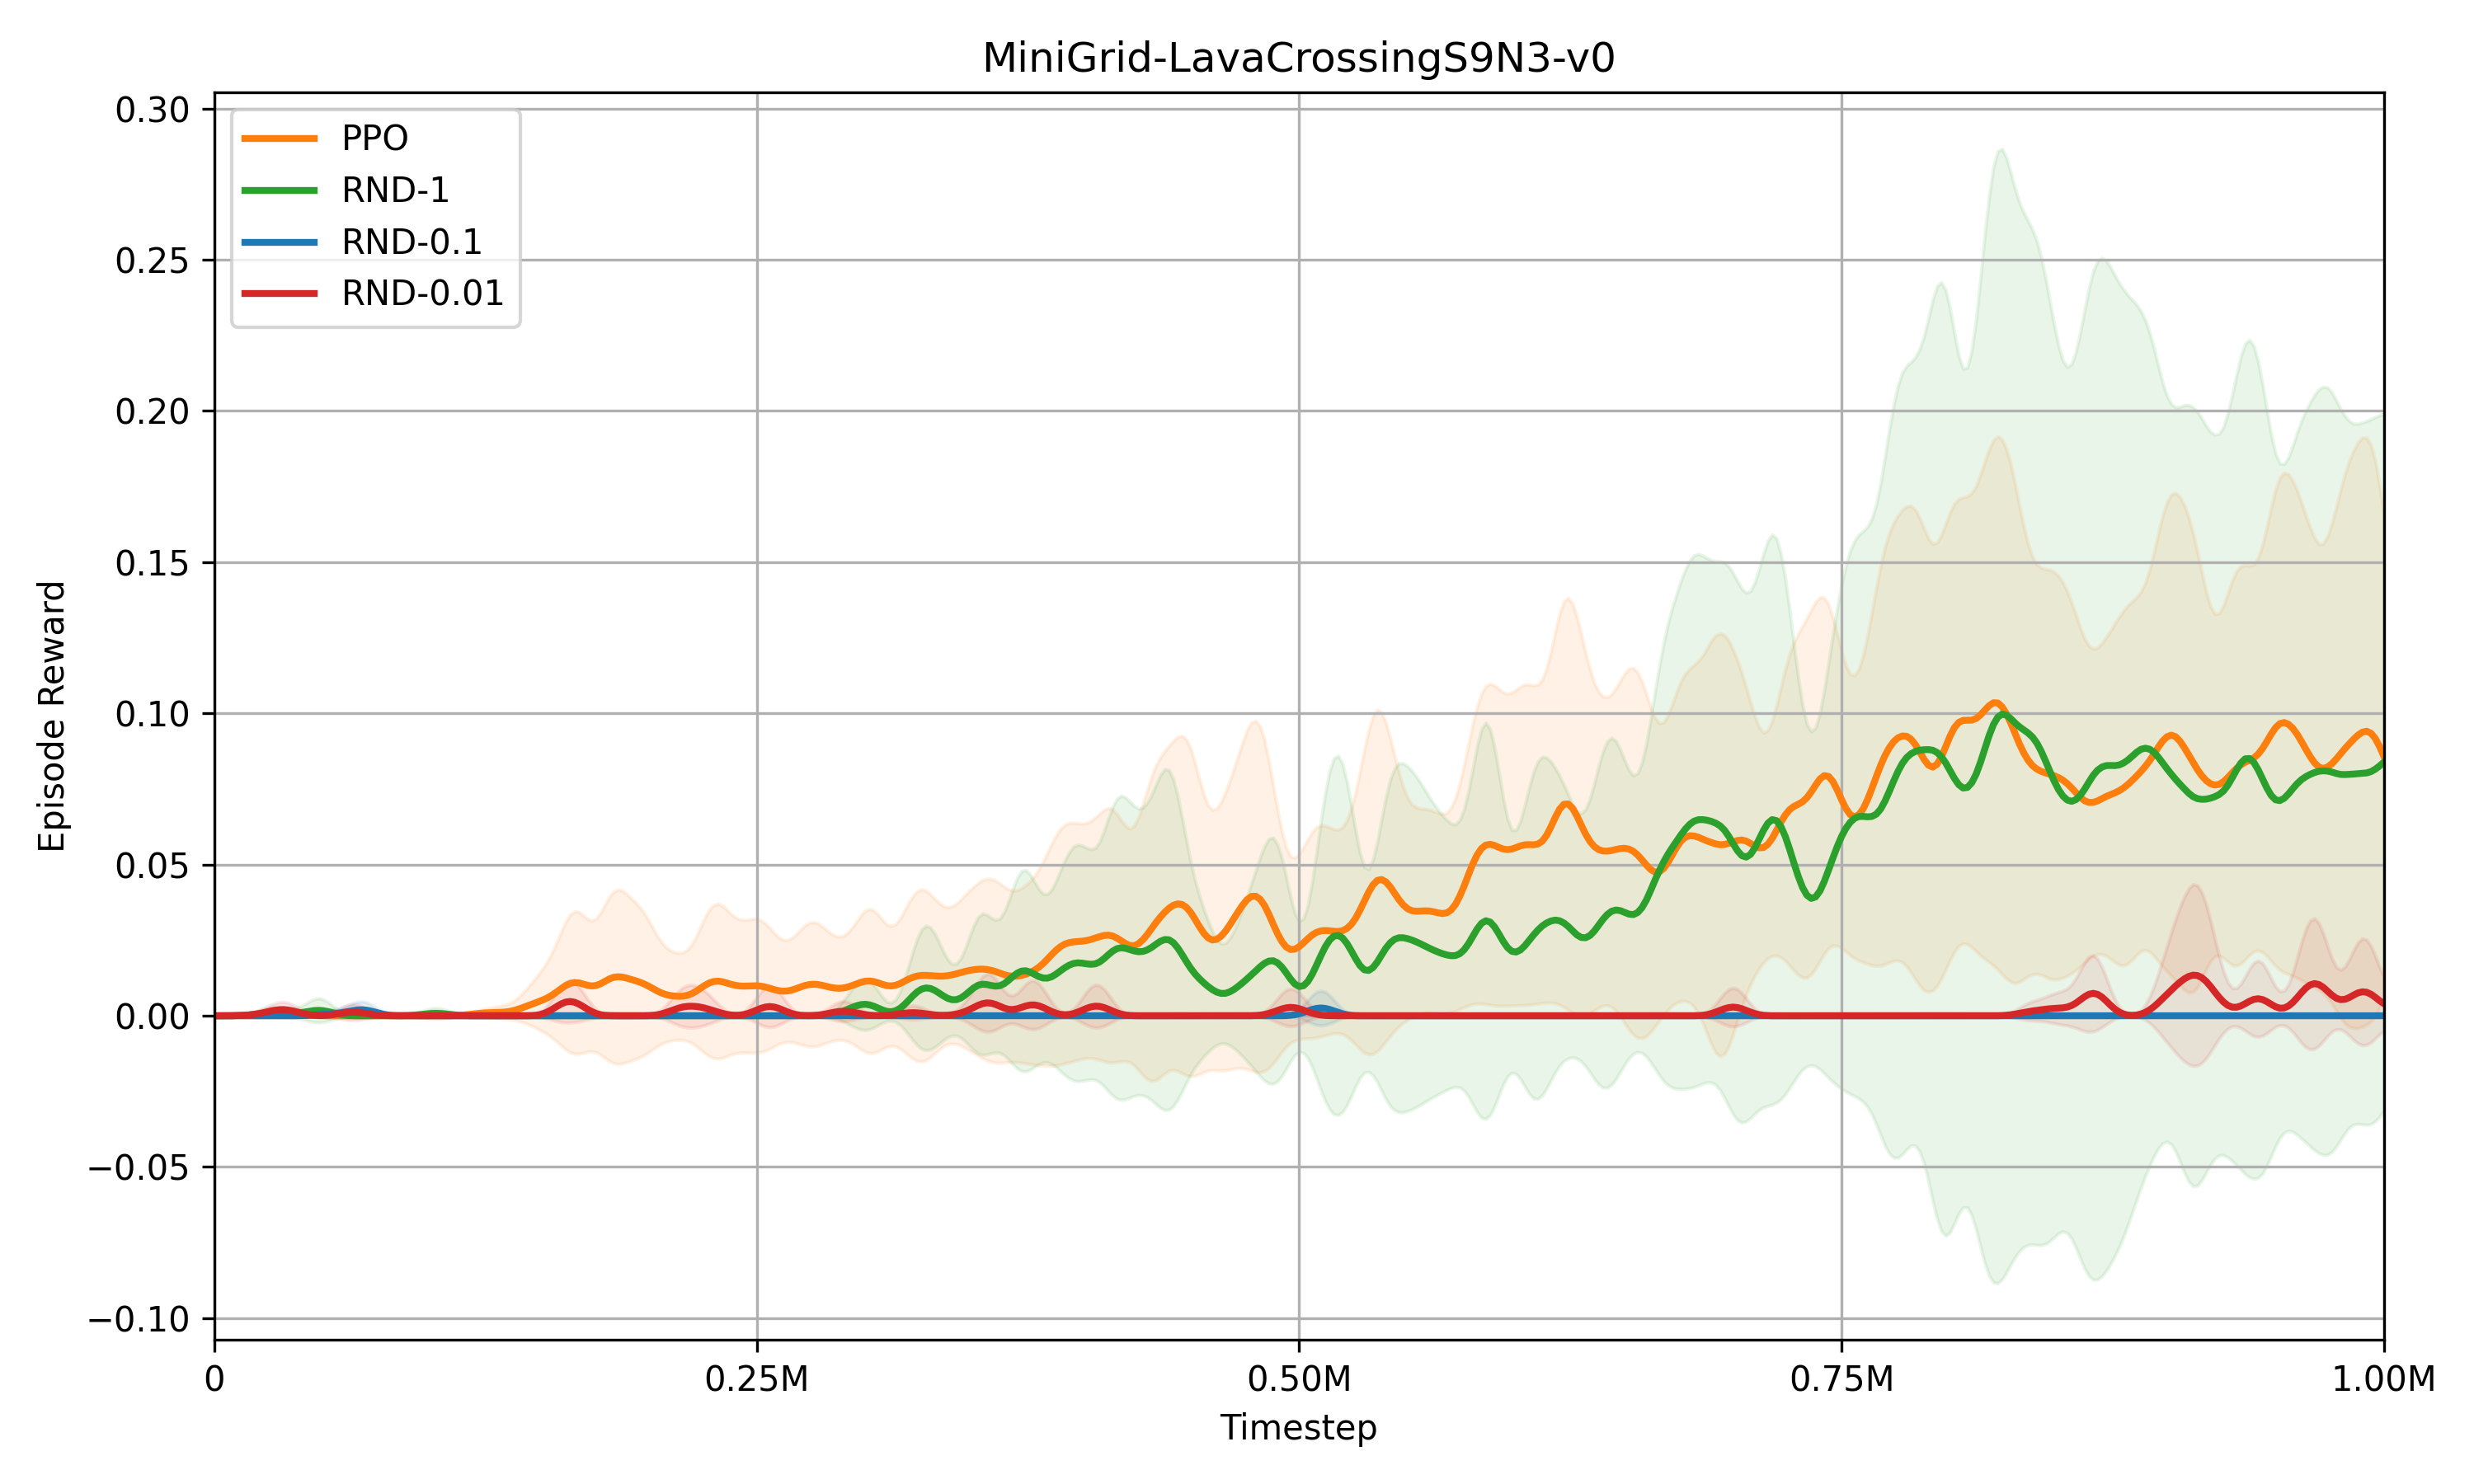
\includegraphics[width=\textwidth]{figs/MiniGrid-LavaCrossingS9N3-v0/episode_reward.png}
    
    (a) Episode Reward
\end{minipage}
\hfill
\begin{minipage}{0.45\textwidth}
    \centering
    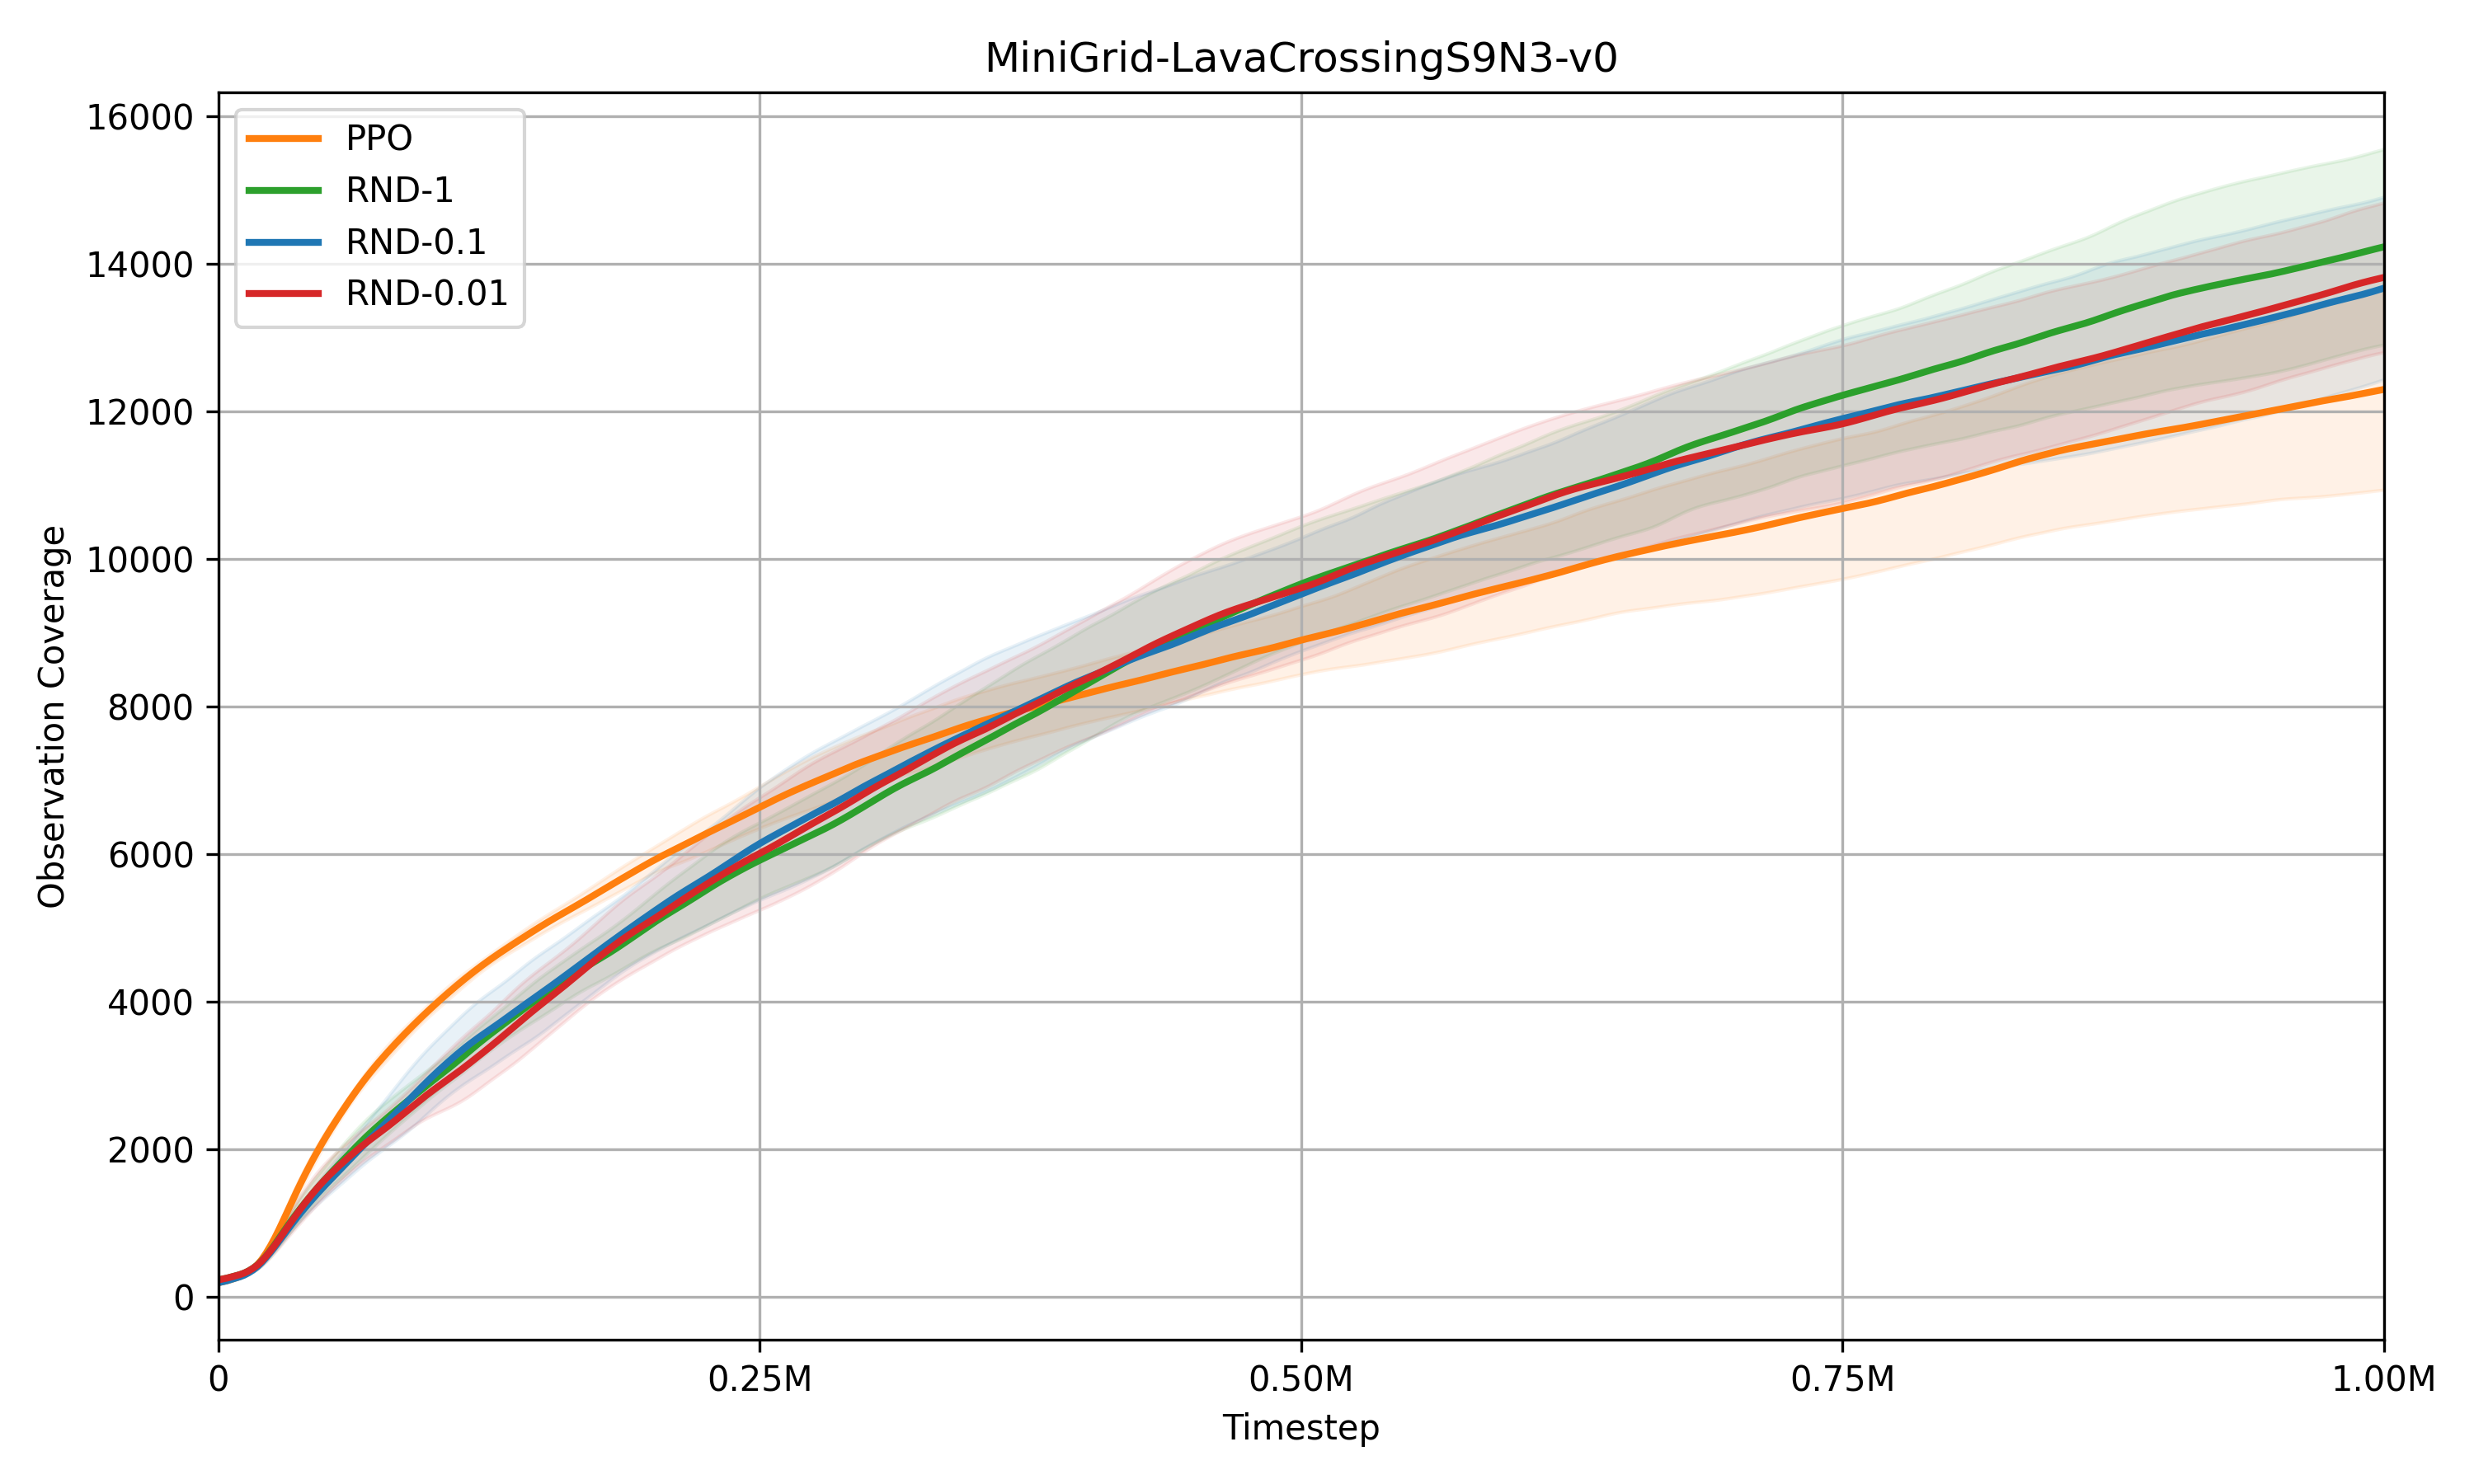
\includegraphics[width=\textwidth]{figs/MiniGrid-LavaCrossingS9N3-v0/obs_coverage.png}
    
    (b) Observation Coverage
\end{minipage}

\vspace{0.3cm}

\begin{minipage}{0.45\textwidth}
    \centering
    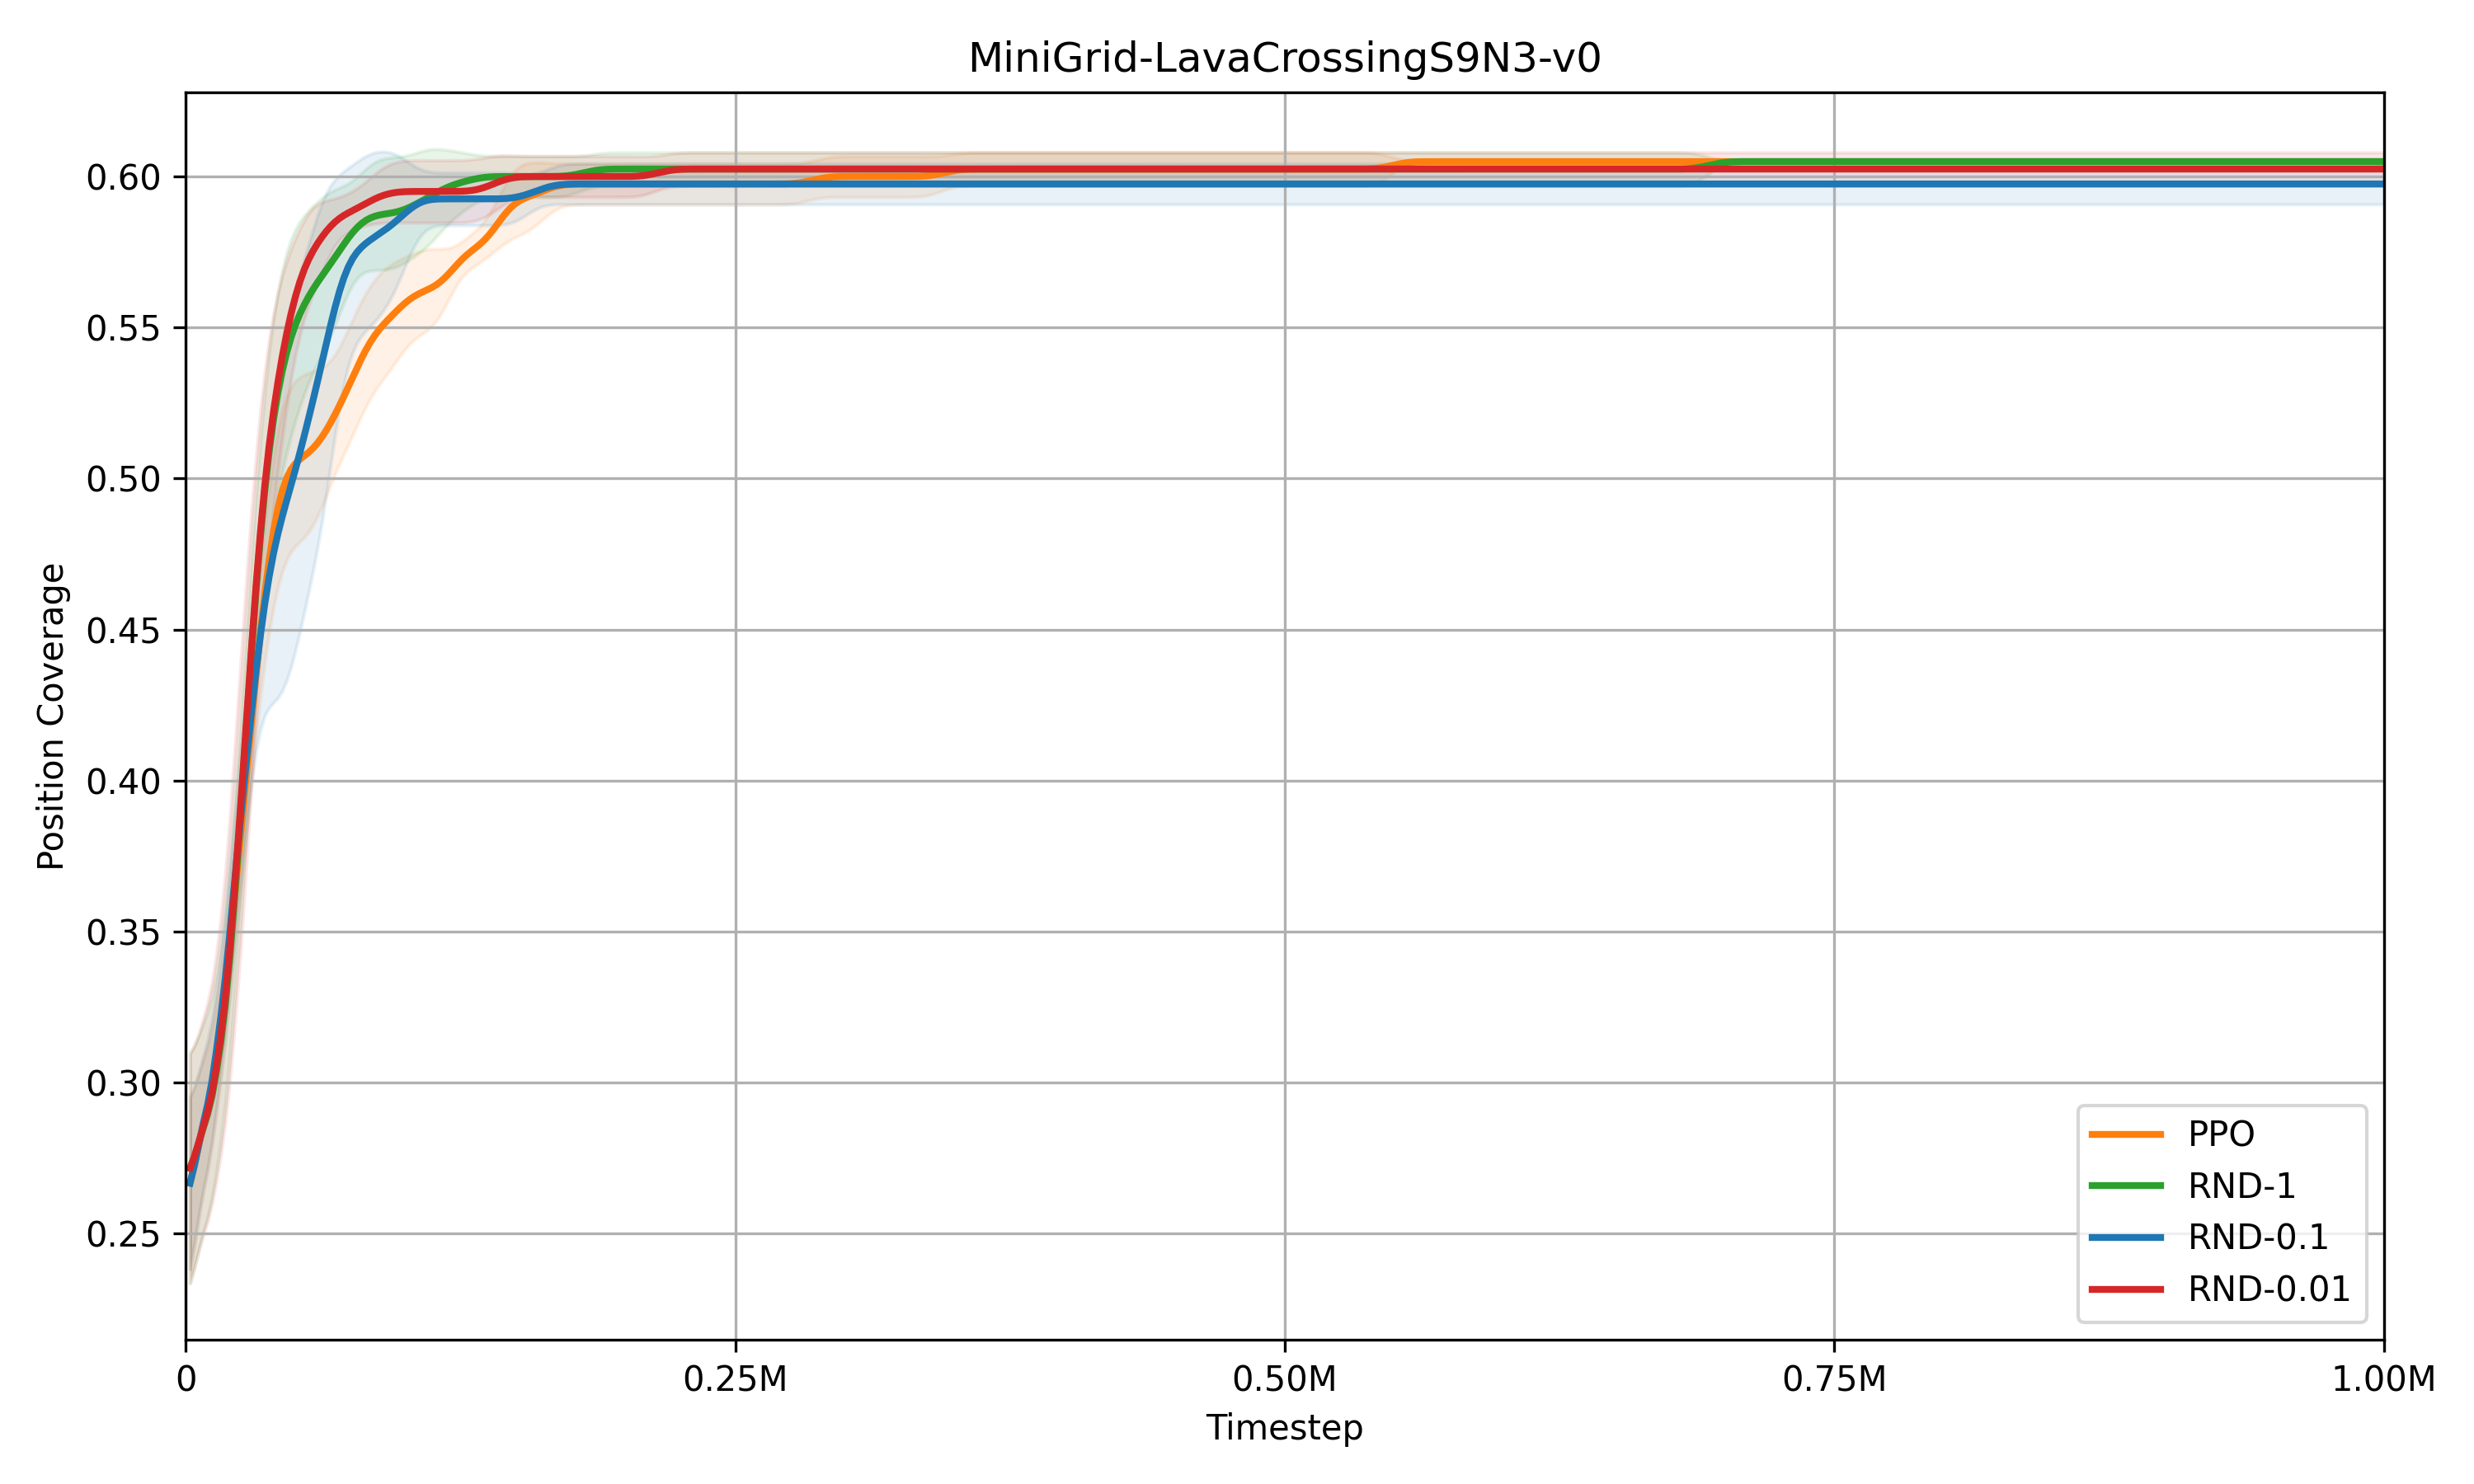
\includegraphics[width=\textwidth]{figs/MiniGrid-LavaCrossingS9N3-v0/pos_coverage.png}
    
    (c) Position Coverage
\end{minipage}
\hfill
\begin{minipage}{0.45\textwidth}
    \centering
    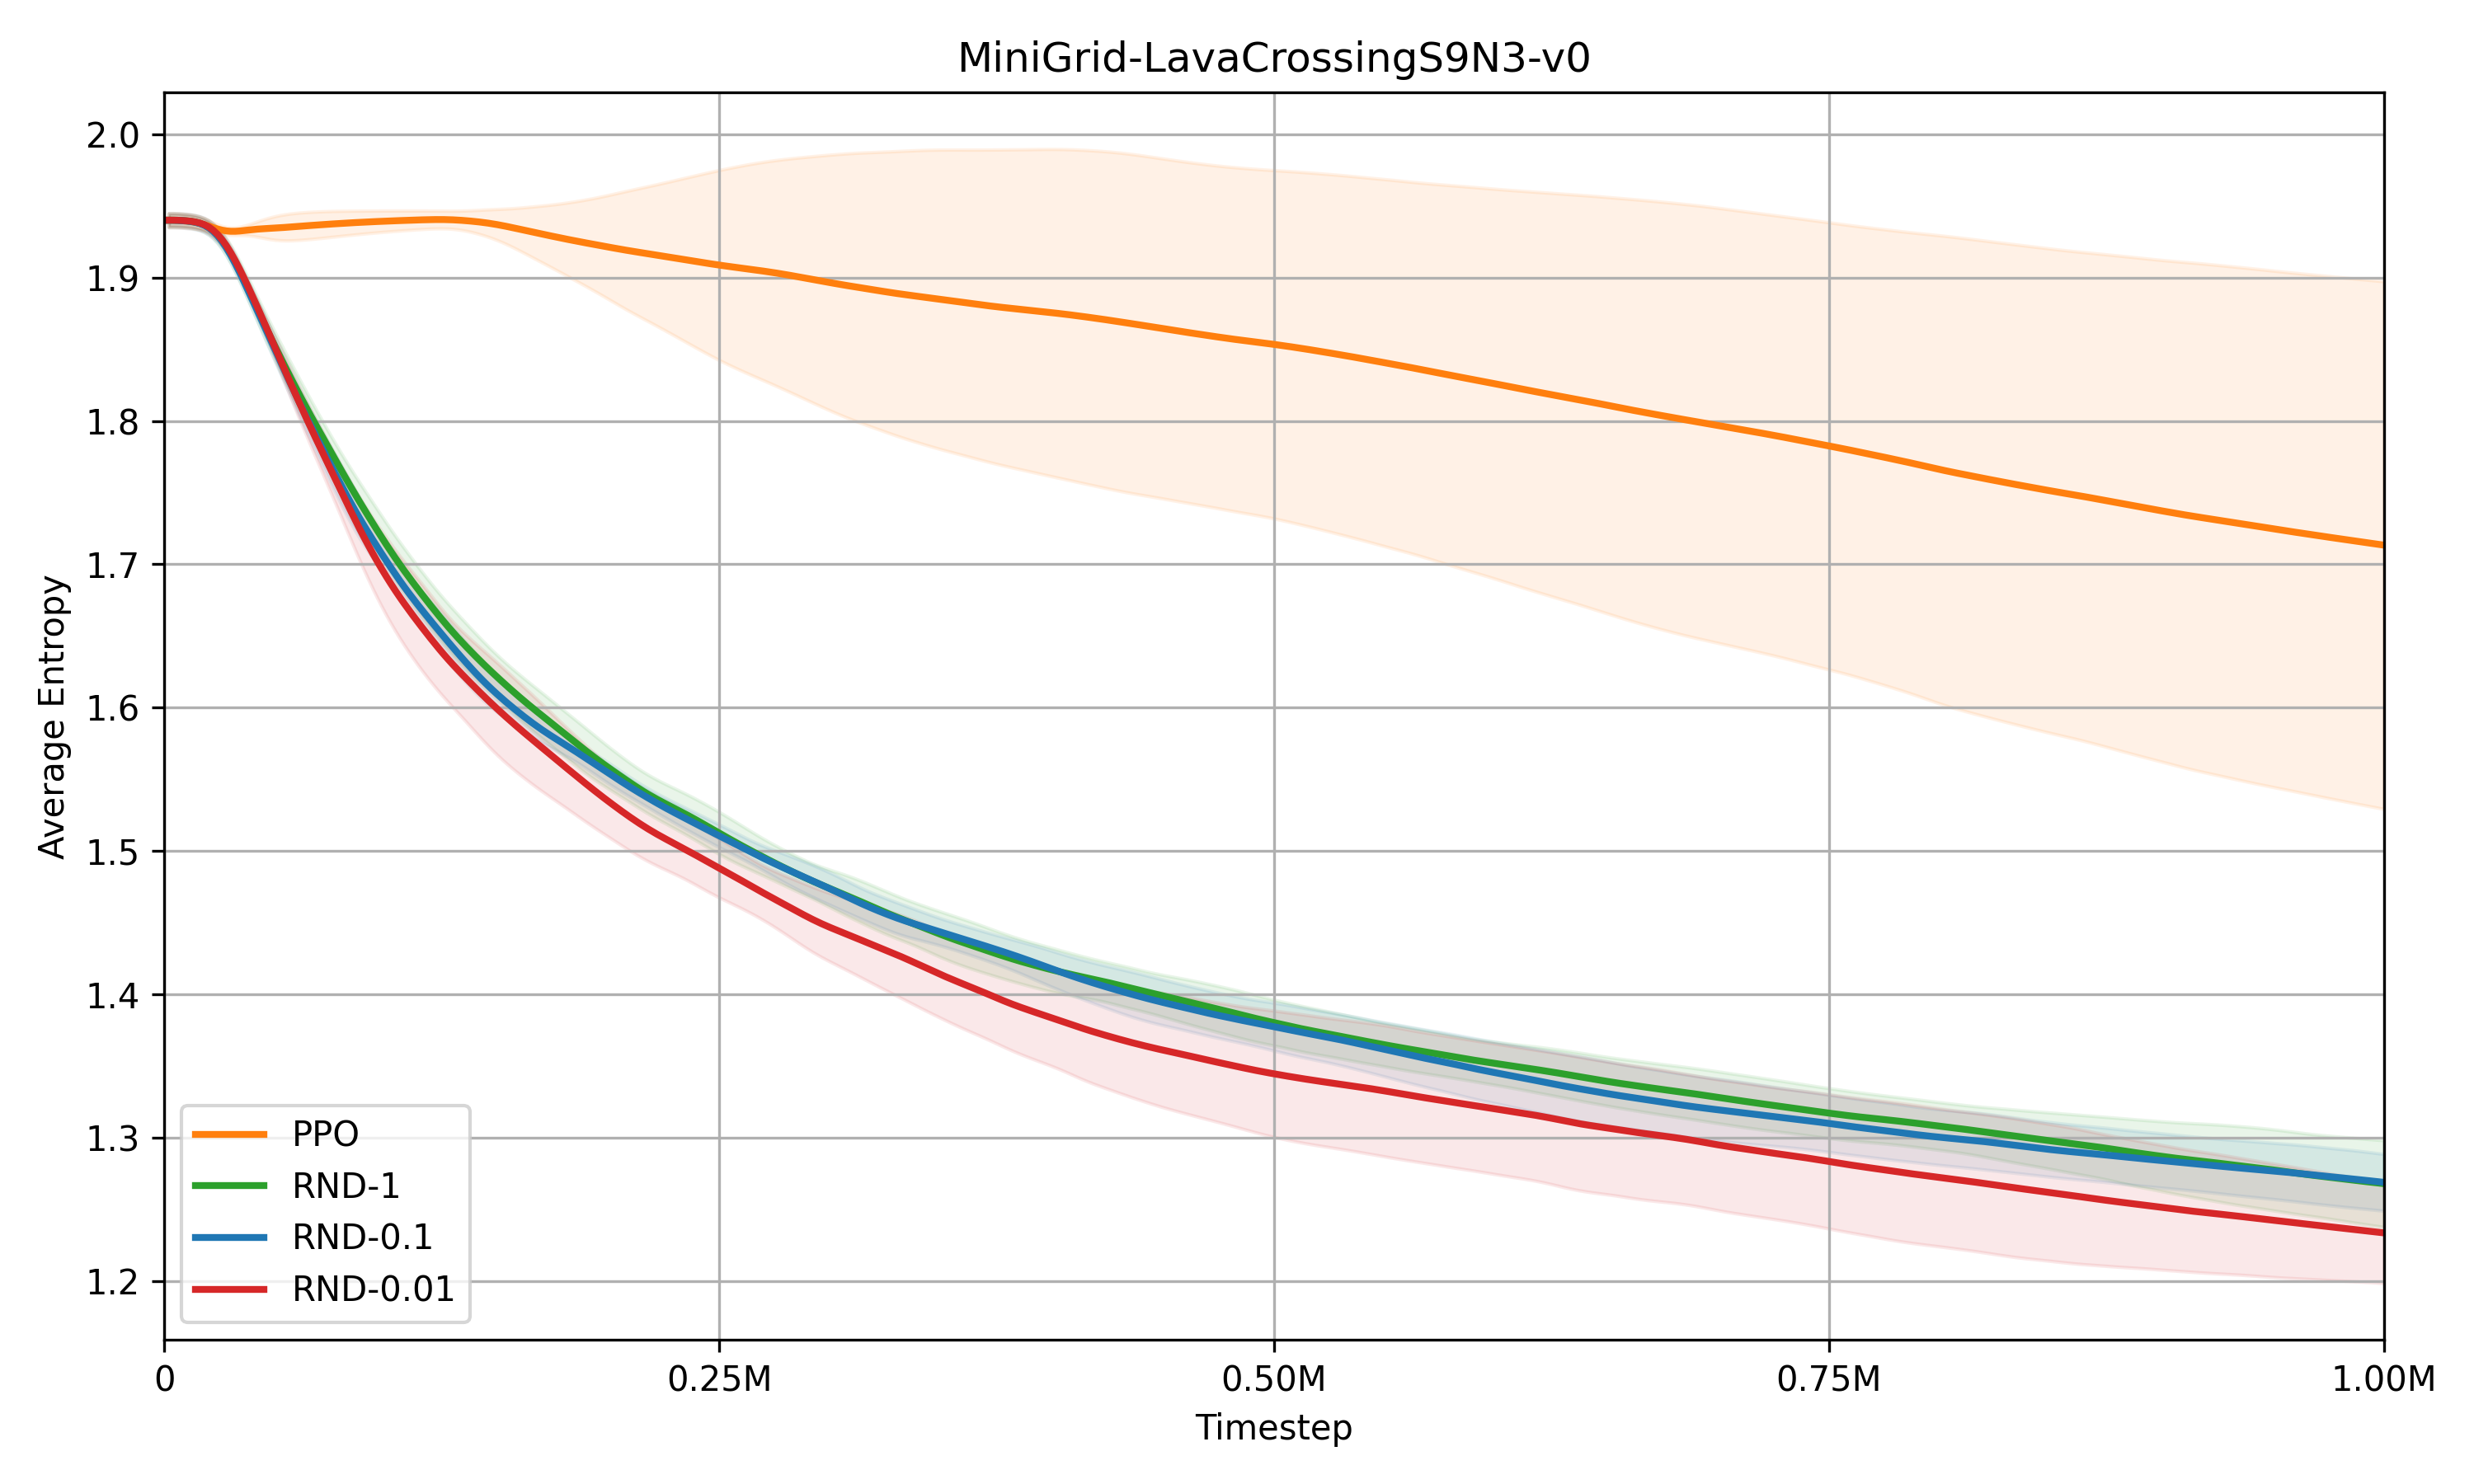
\includegraphics[width=\textwidth]{figs/MiniGrid-LavaCrossingS9N3-v0/avg_entropy.png}
    
    (d) Policy Entropy
\end{minipage}
\end{figure}

\subsection{Kết quả của RQ2}

\begin{figure}[H]{Các chỉ số huấn luyện trên DoorKey-5x5}
\centering
\begin{minipage}{0.45\textwidth}
    \centering
    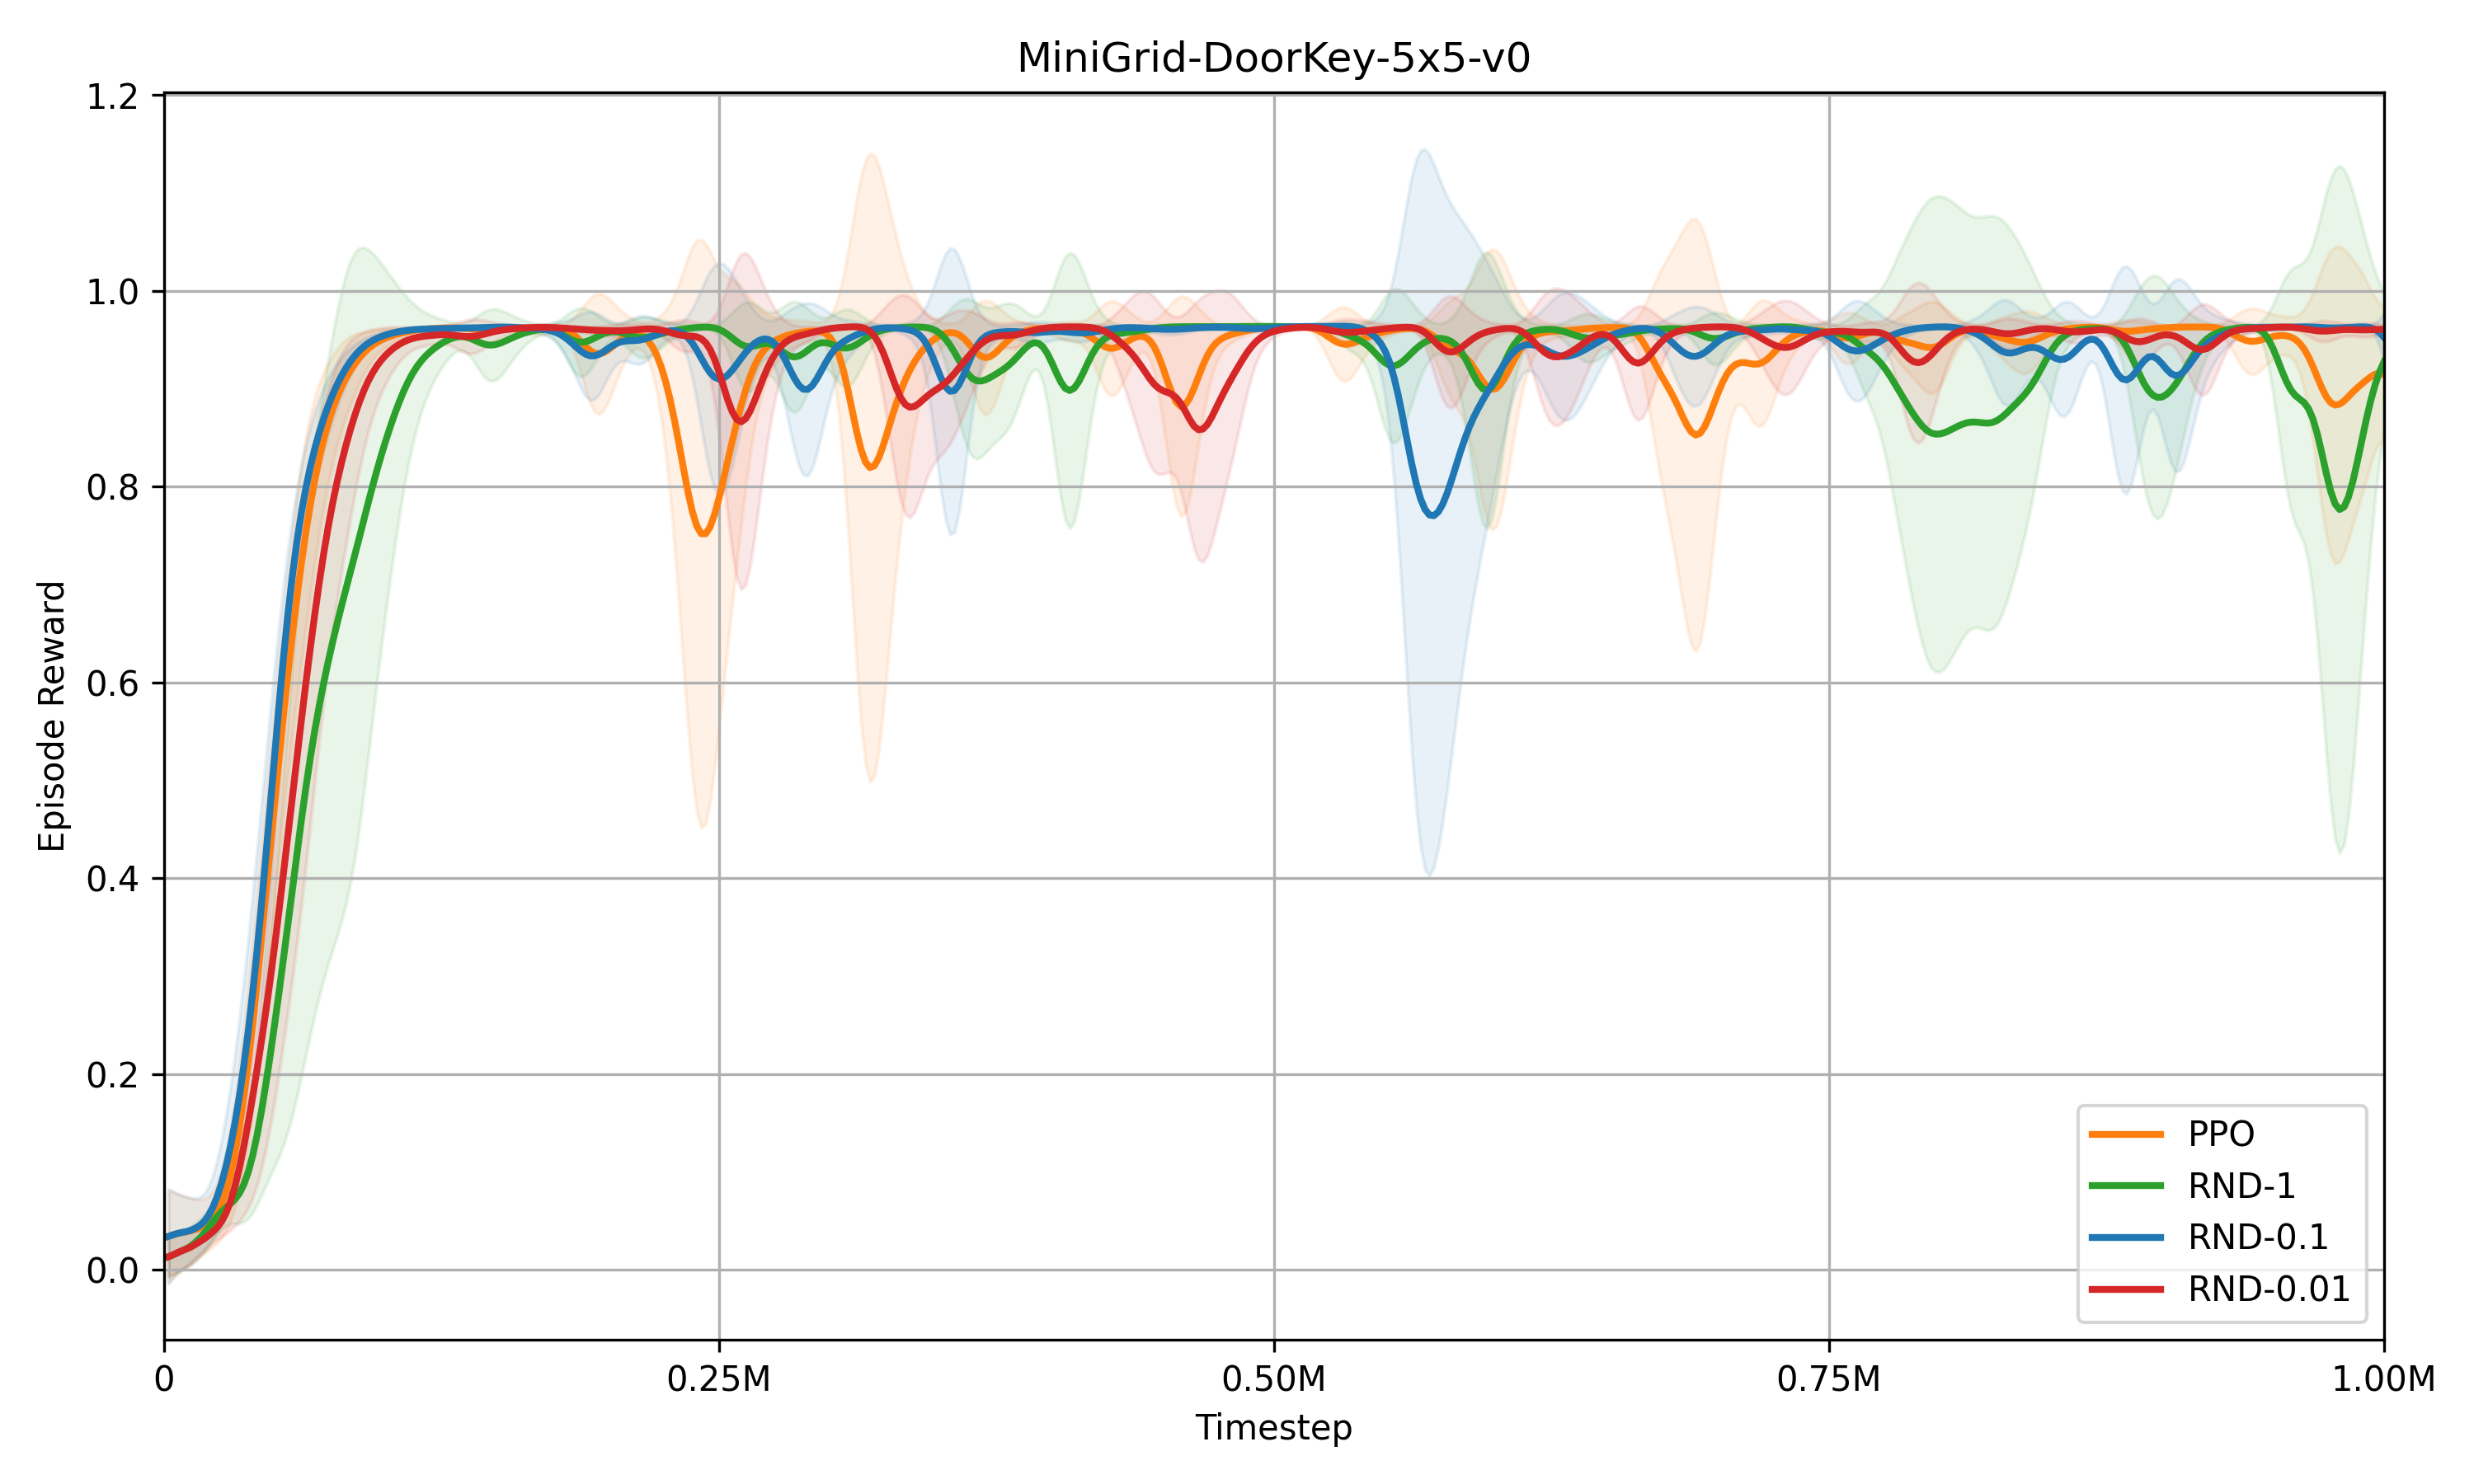
\includegraphics[width=\textwidth]{figs/MiniGrid-DoorKey-5x5-v0/episode_reward.png}
    
    (a) Episode Reward
\end{minipage}
\hfill
\begin{minipage}{0.45\textwidth}
    \centering
    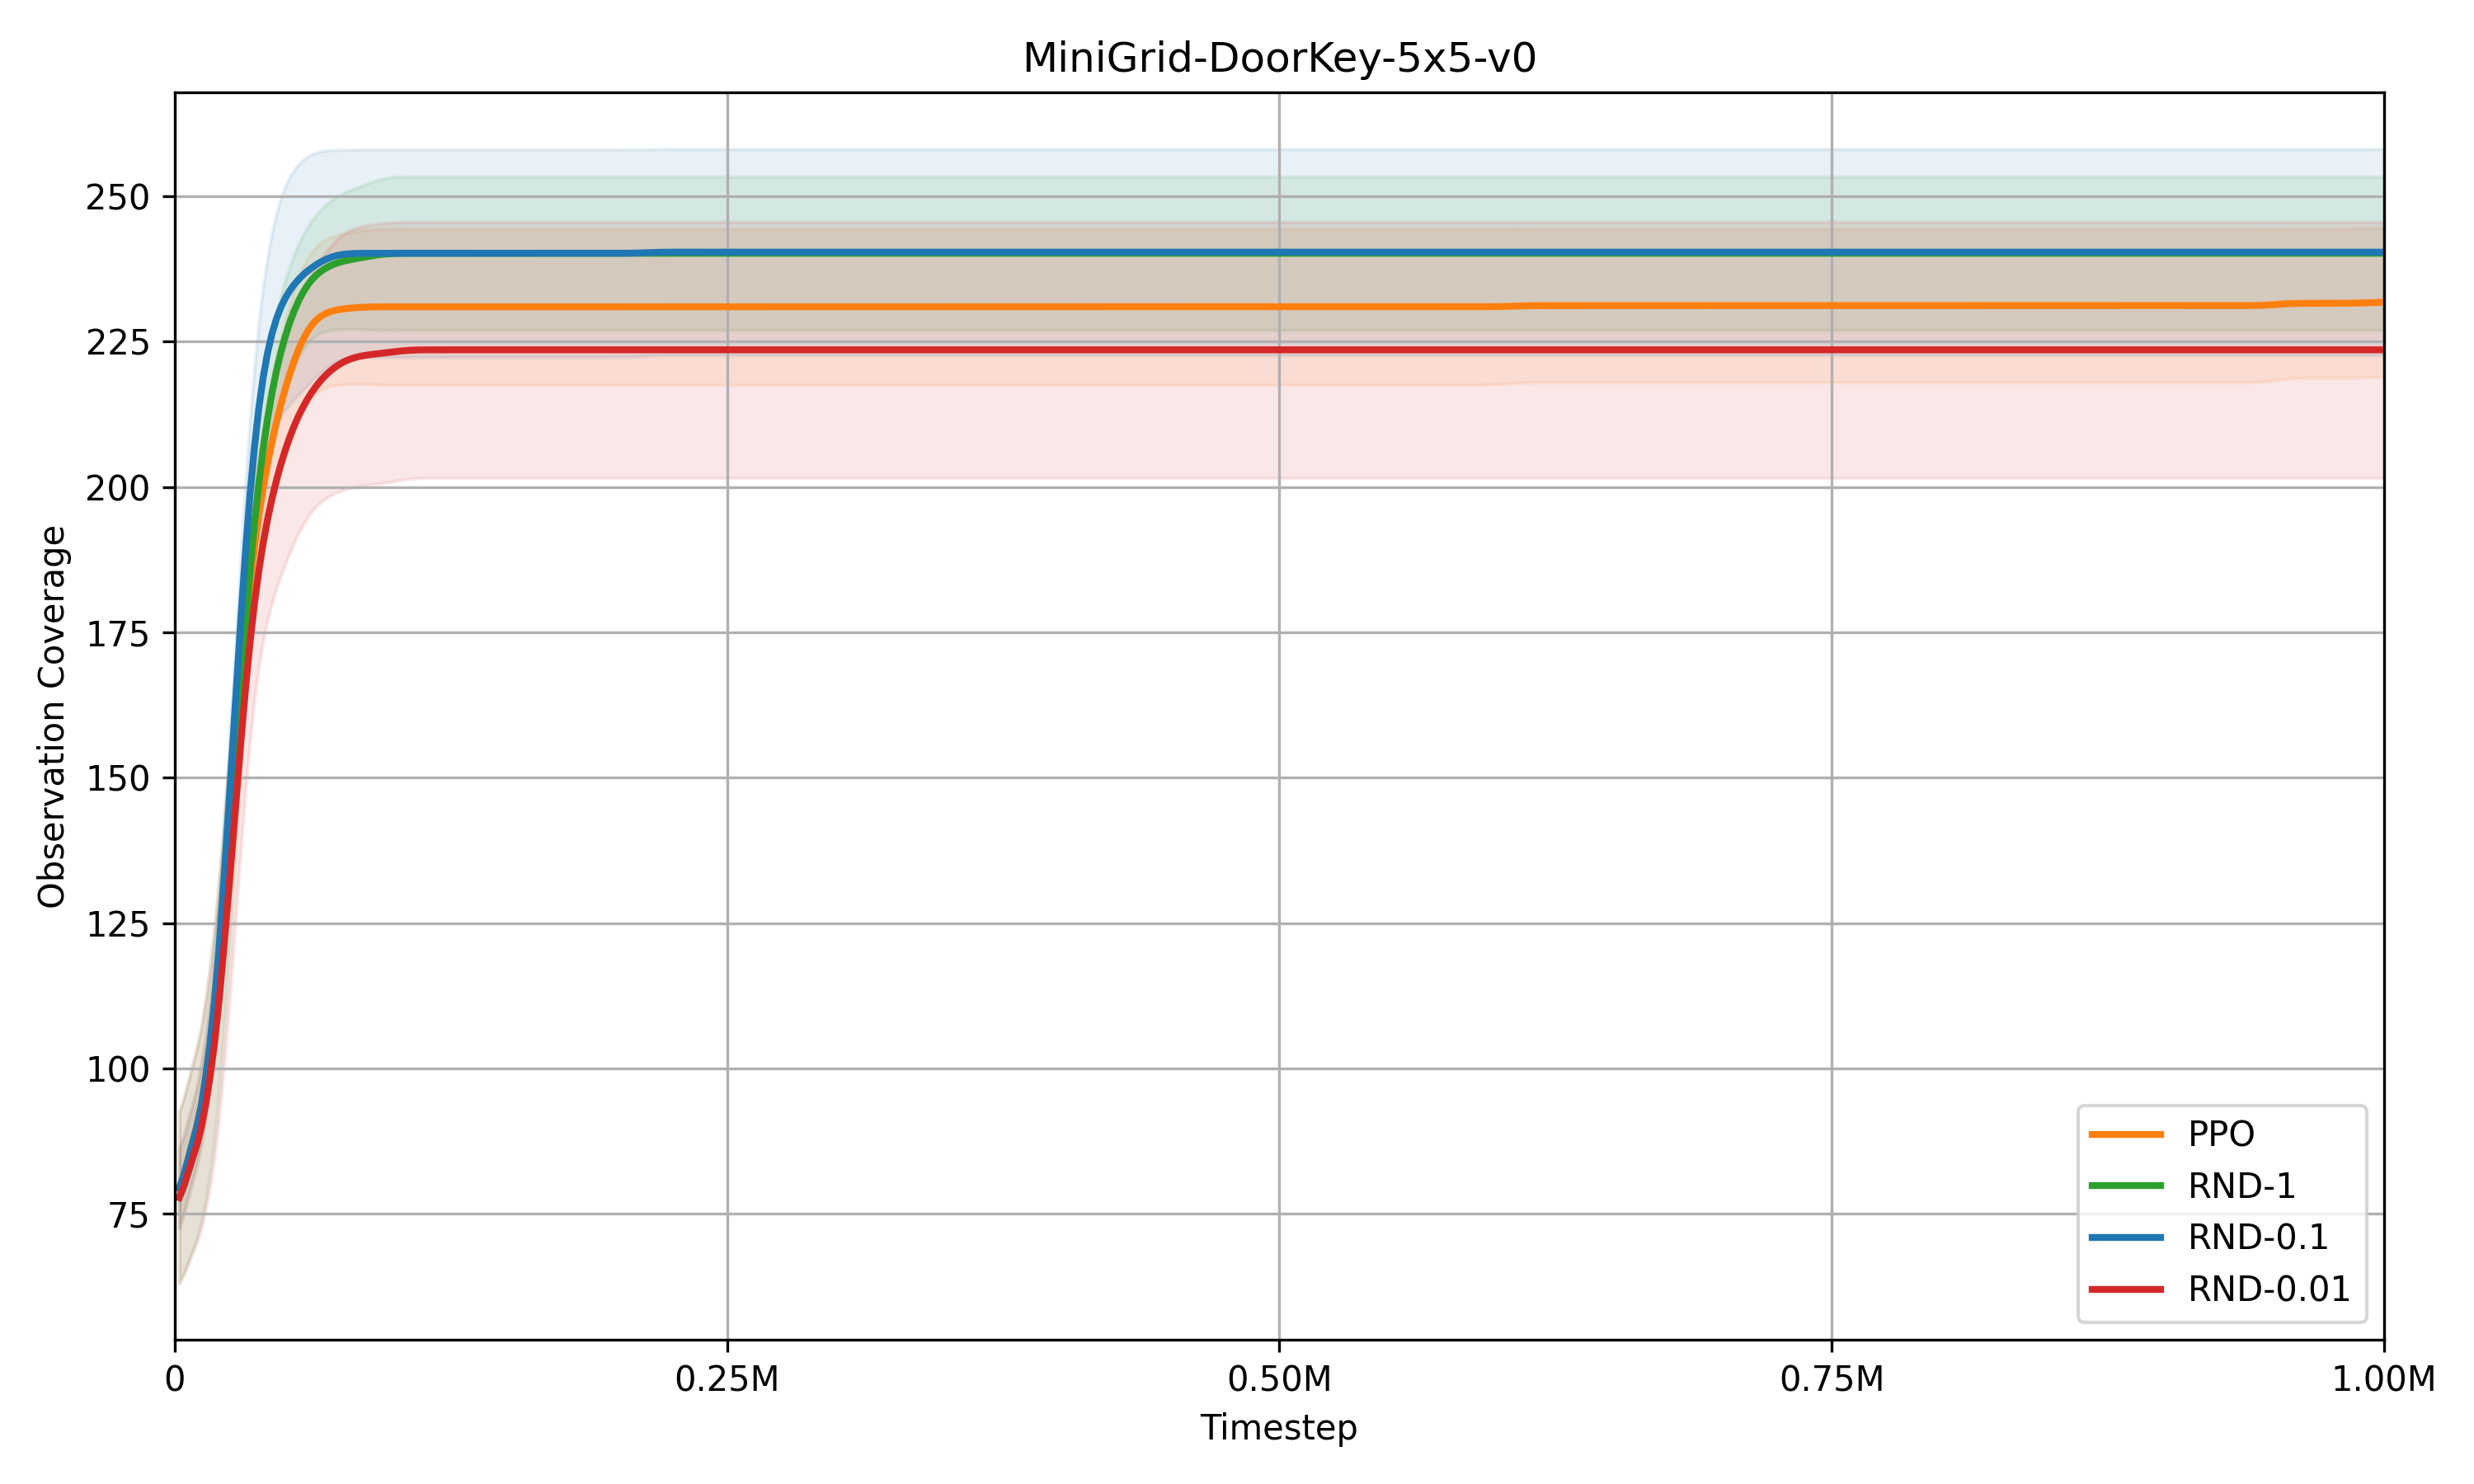
\includegraphics[width=\textwidth]{figs/MiniGrid-DoorKey-5x5-v0/obs_coverage.png}
    
    (b) Observation Coverage
\end{minipage}

\vspace{0.3cm}

\begin{minipage}{0.45\textwidth}
    \centering
    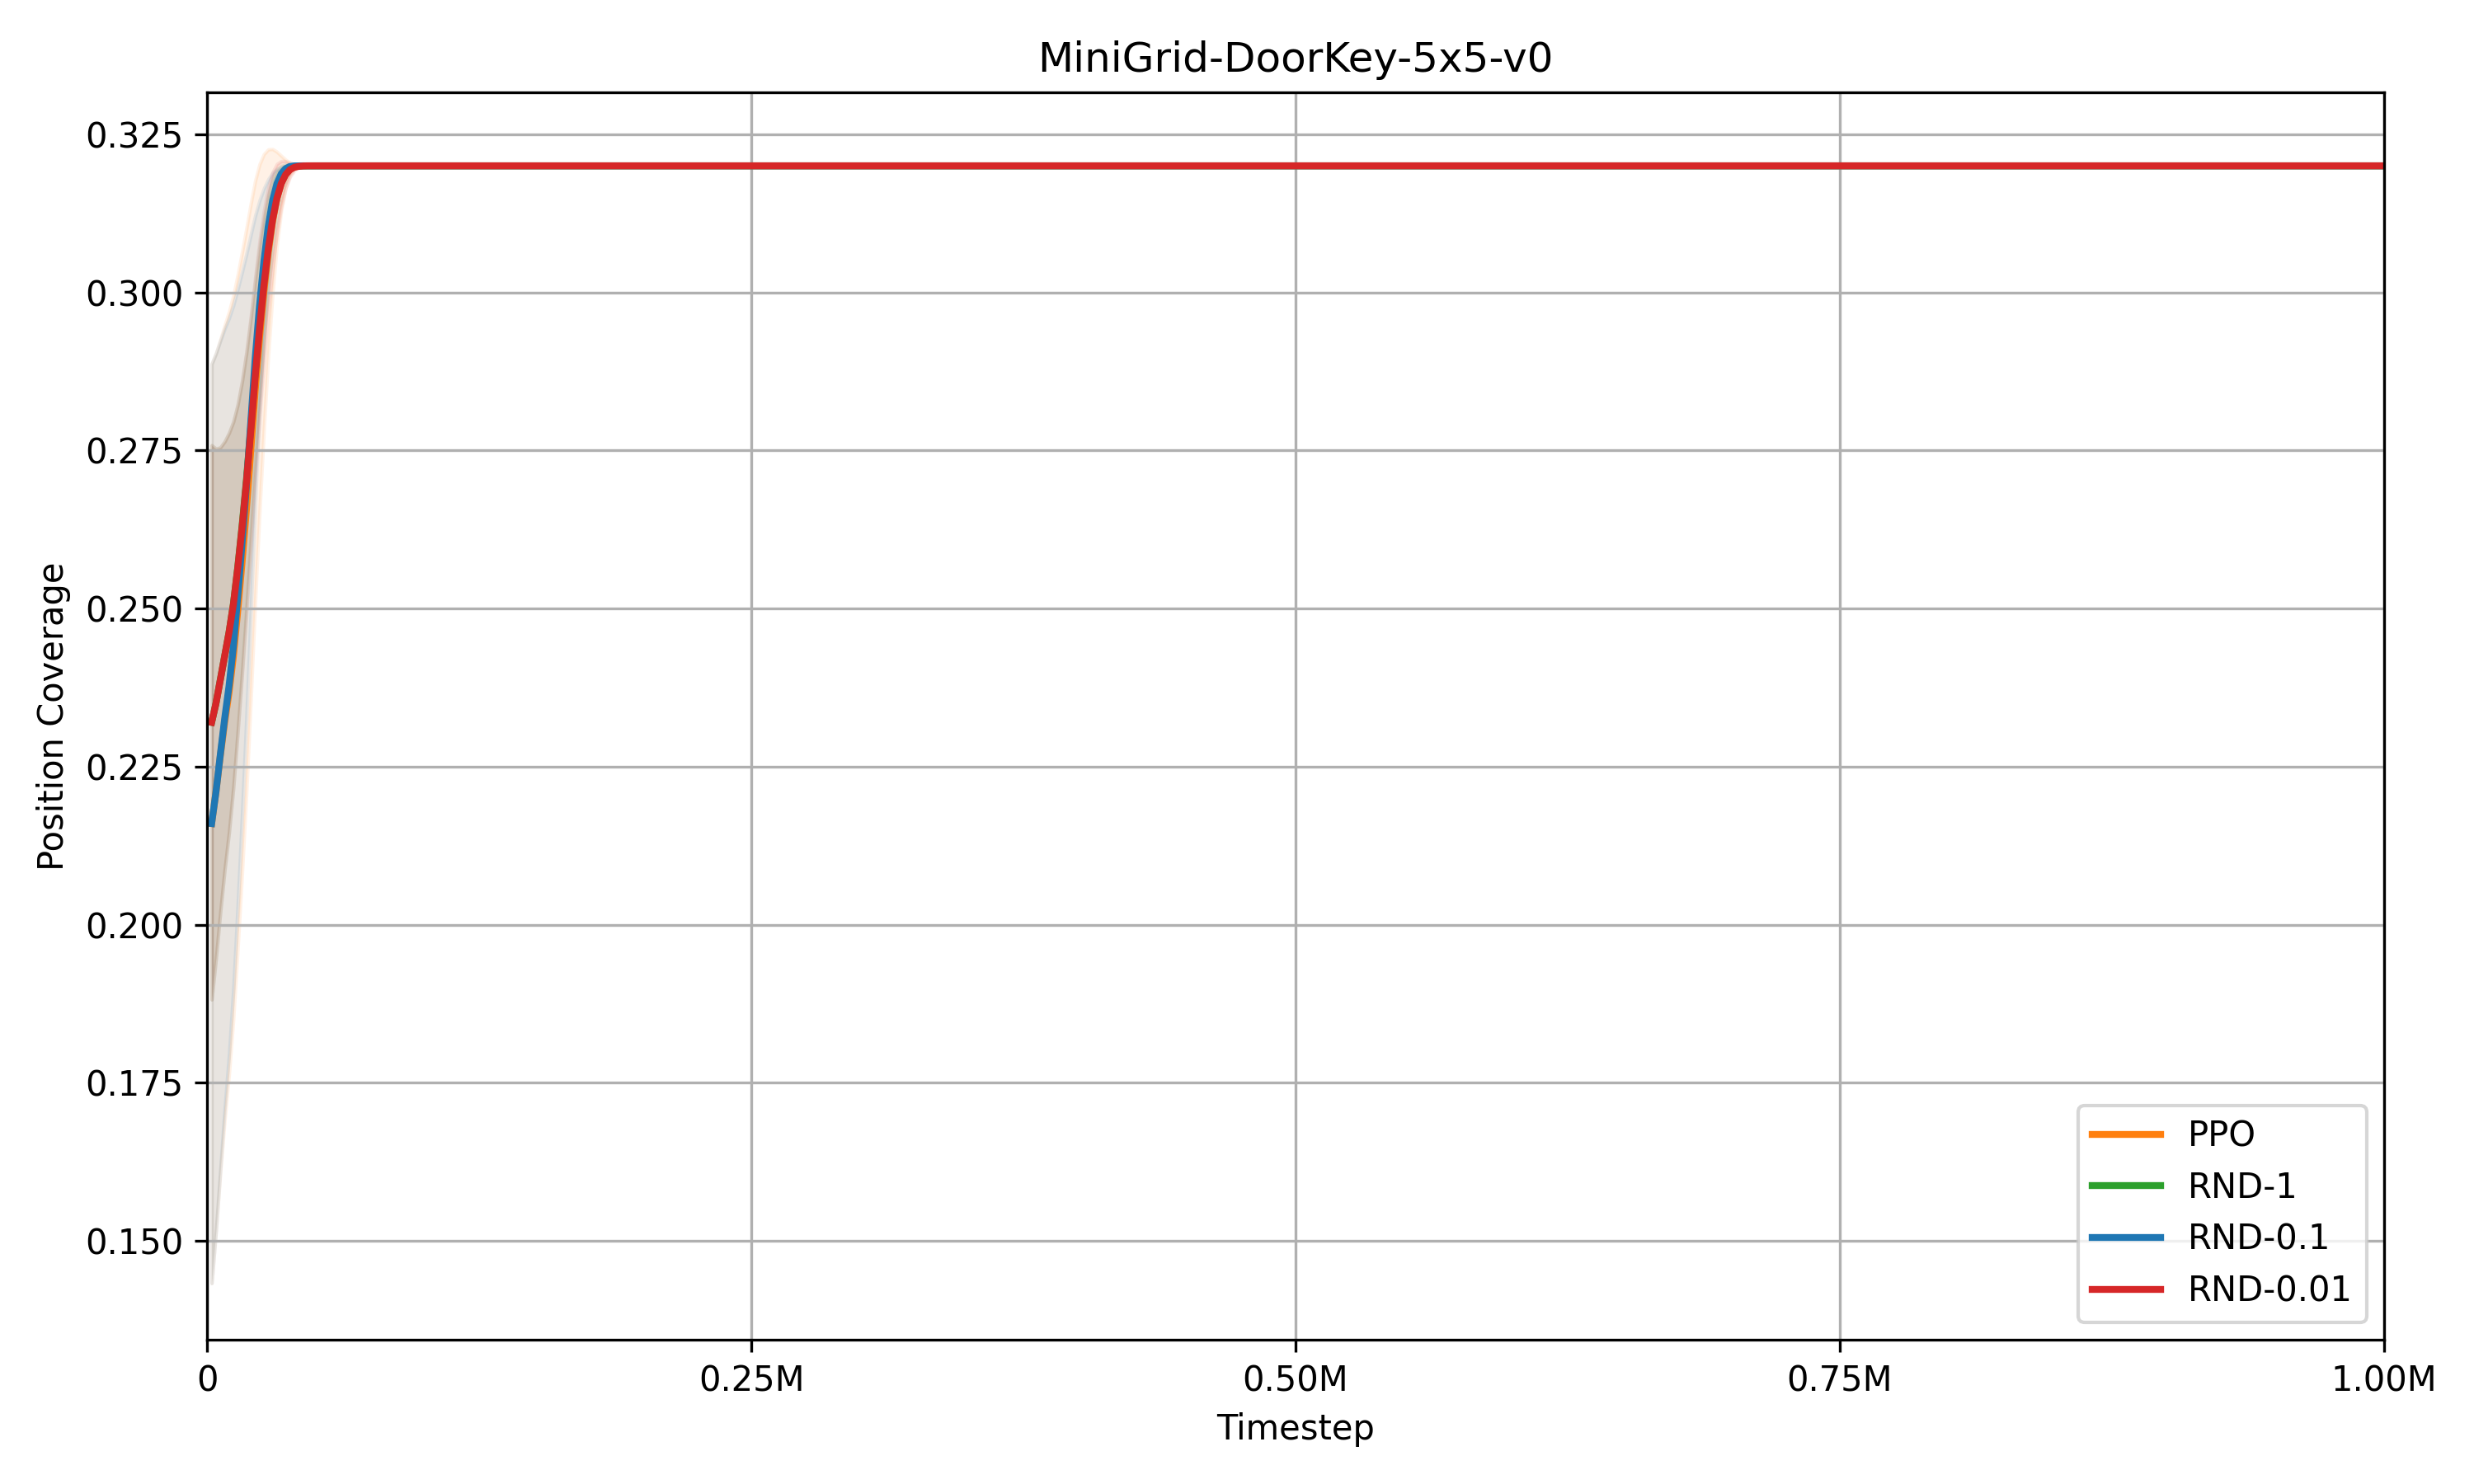
\includegraphics[width=\textwidth]{figs/MiniGrid-DoorKey-5x5-v0/pos_coverage.png}
    
    (c) Position Coverage
\end{minipage}
\hfill
\begin{minipage}{0.45\textwidth}
    \centering
    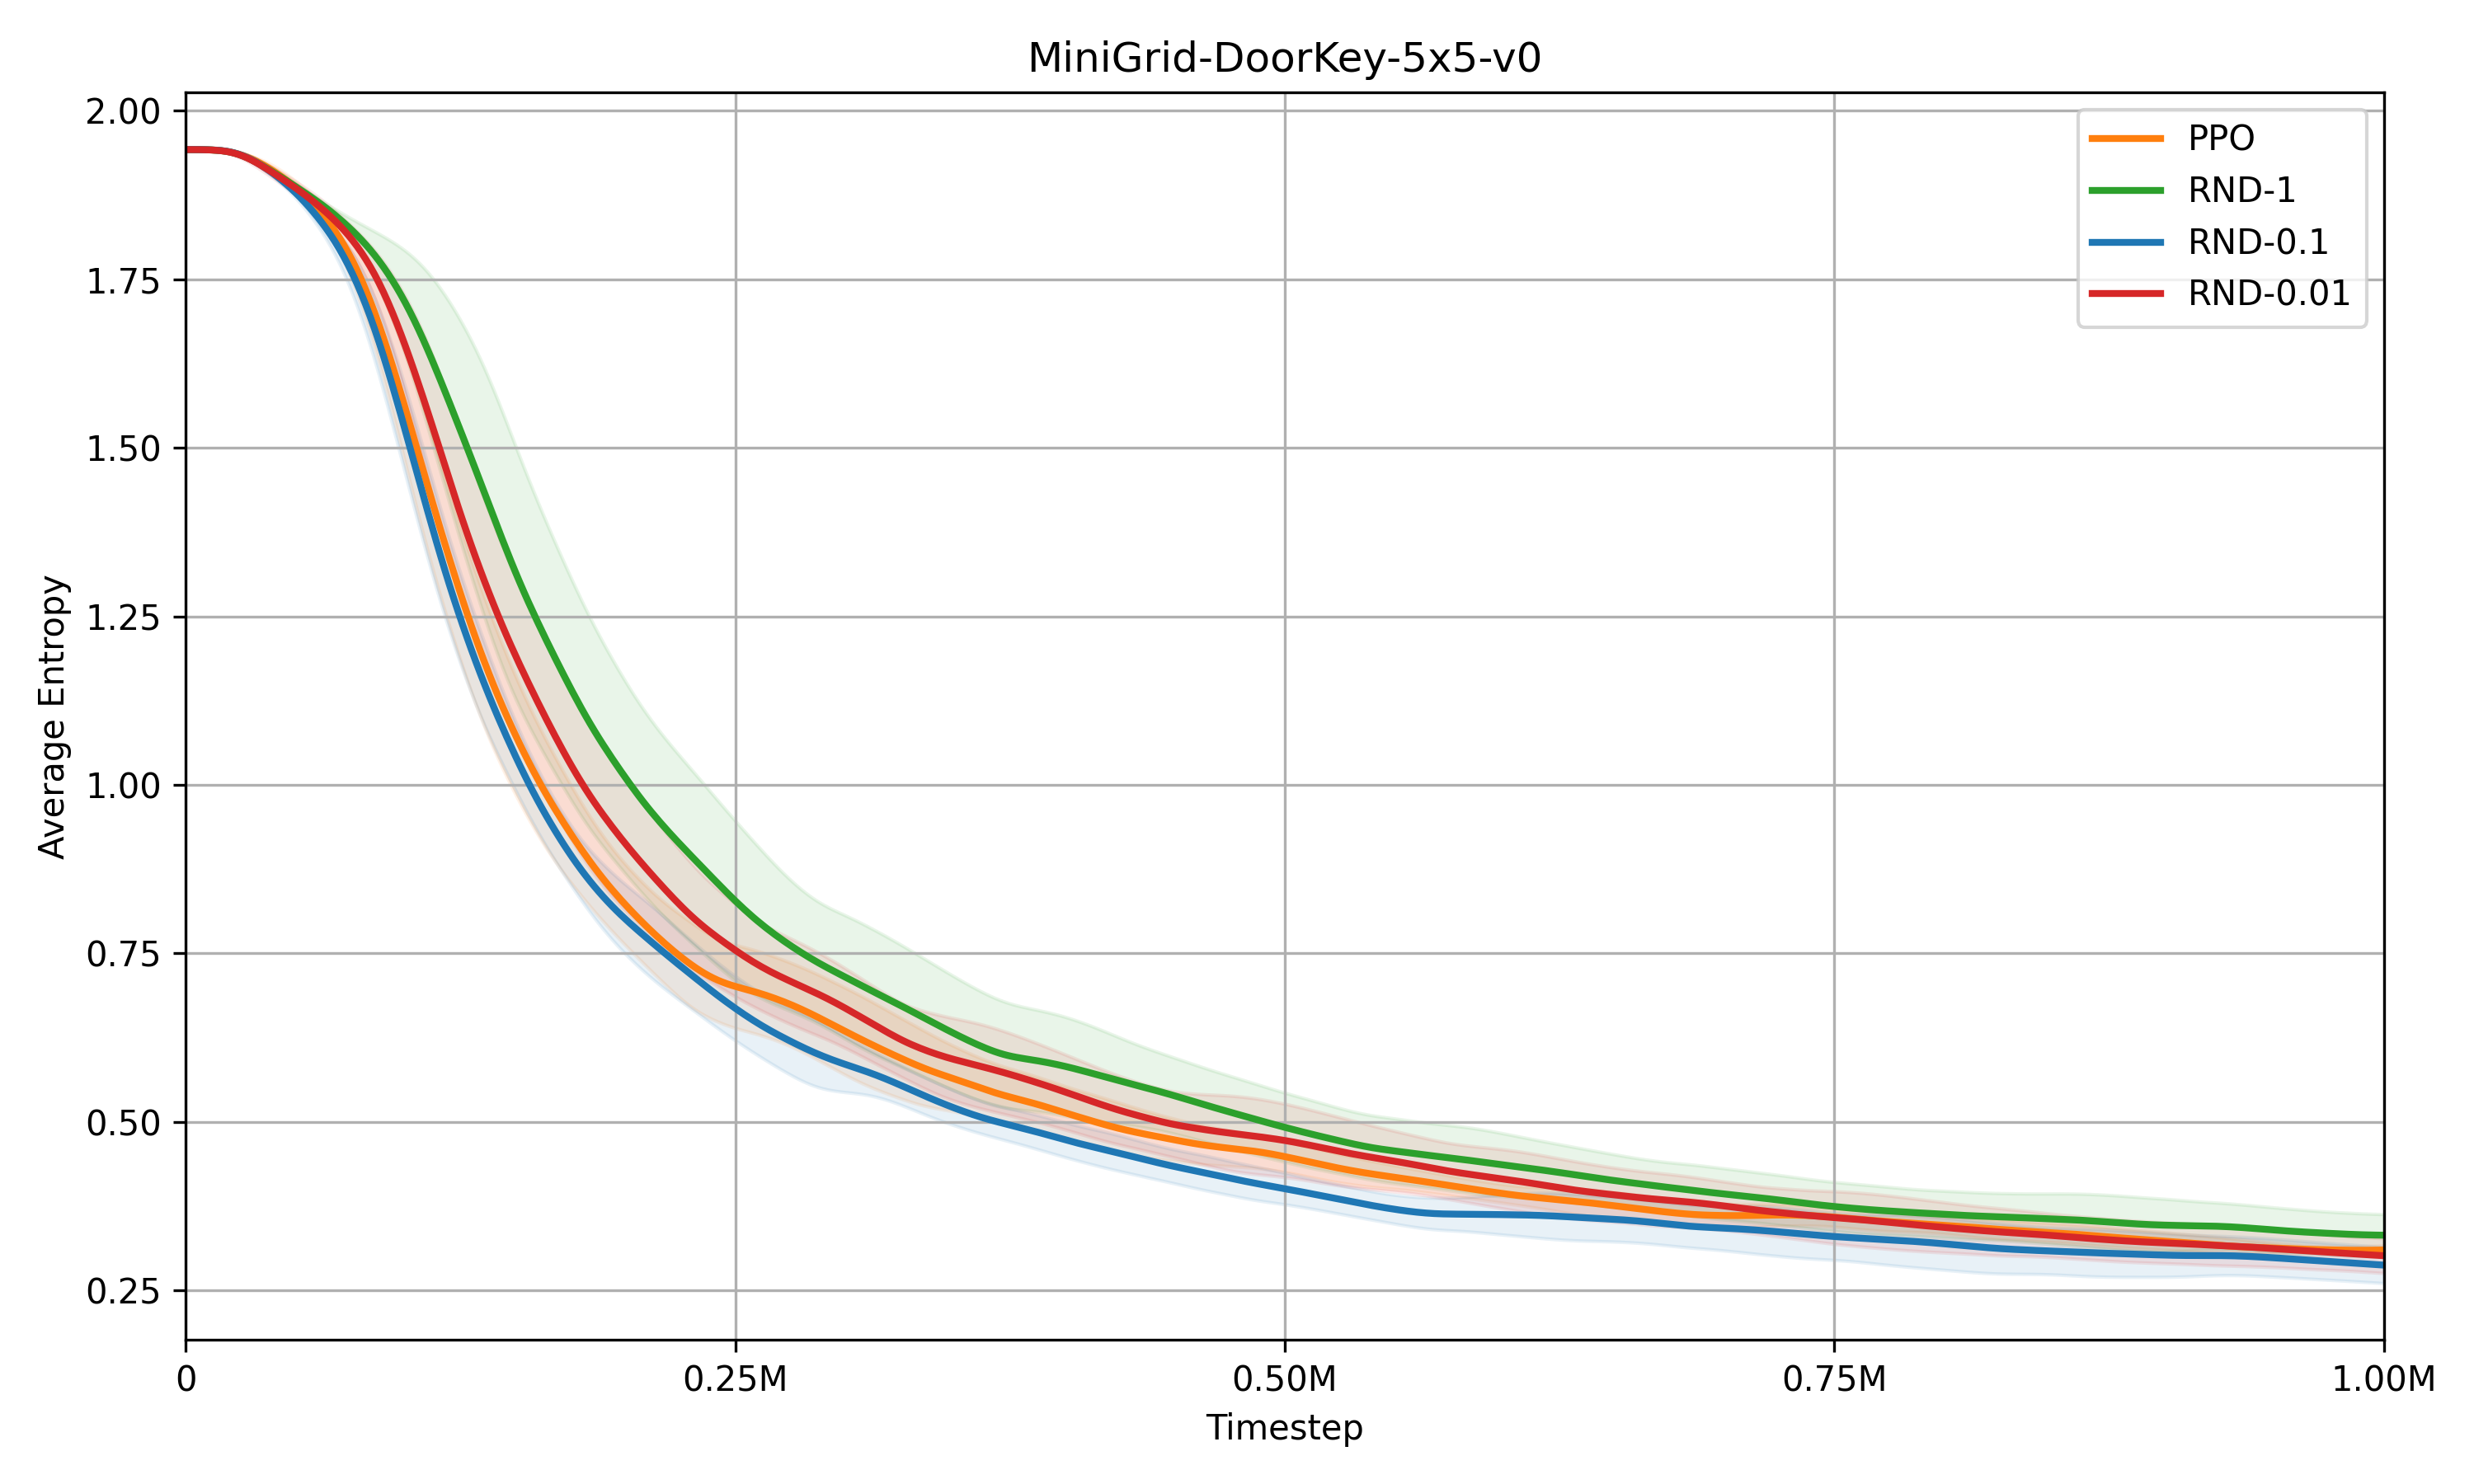
\includegraphics[width=\textwidth]{figs/MiniGrid-DoorKey-5x5-v0/avg_entropy.png}
    
    (d) Policy Entropy
\end{minipage}
\end{figure}

\begin{figure}[H]{Các chỉ số huấn luyện trên DoorKey-6x6}
\centering
\begin{minipage}{0.45\textwidth}
    \centering
    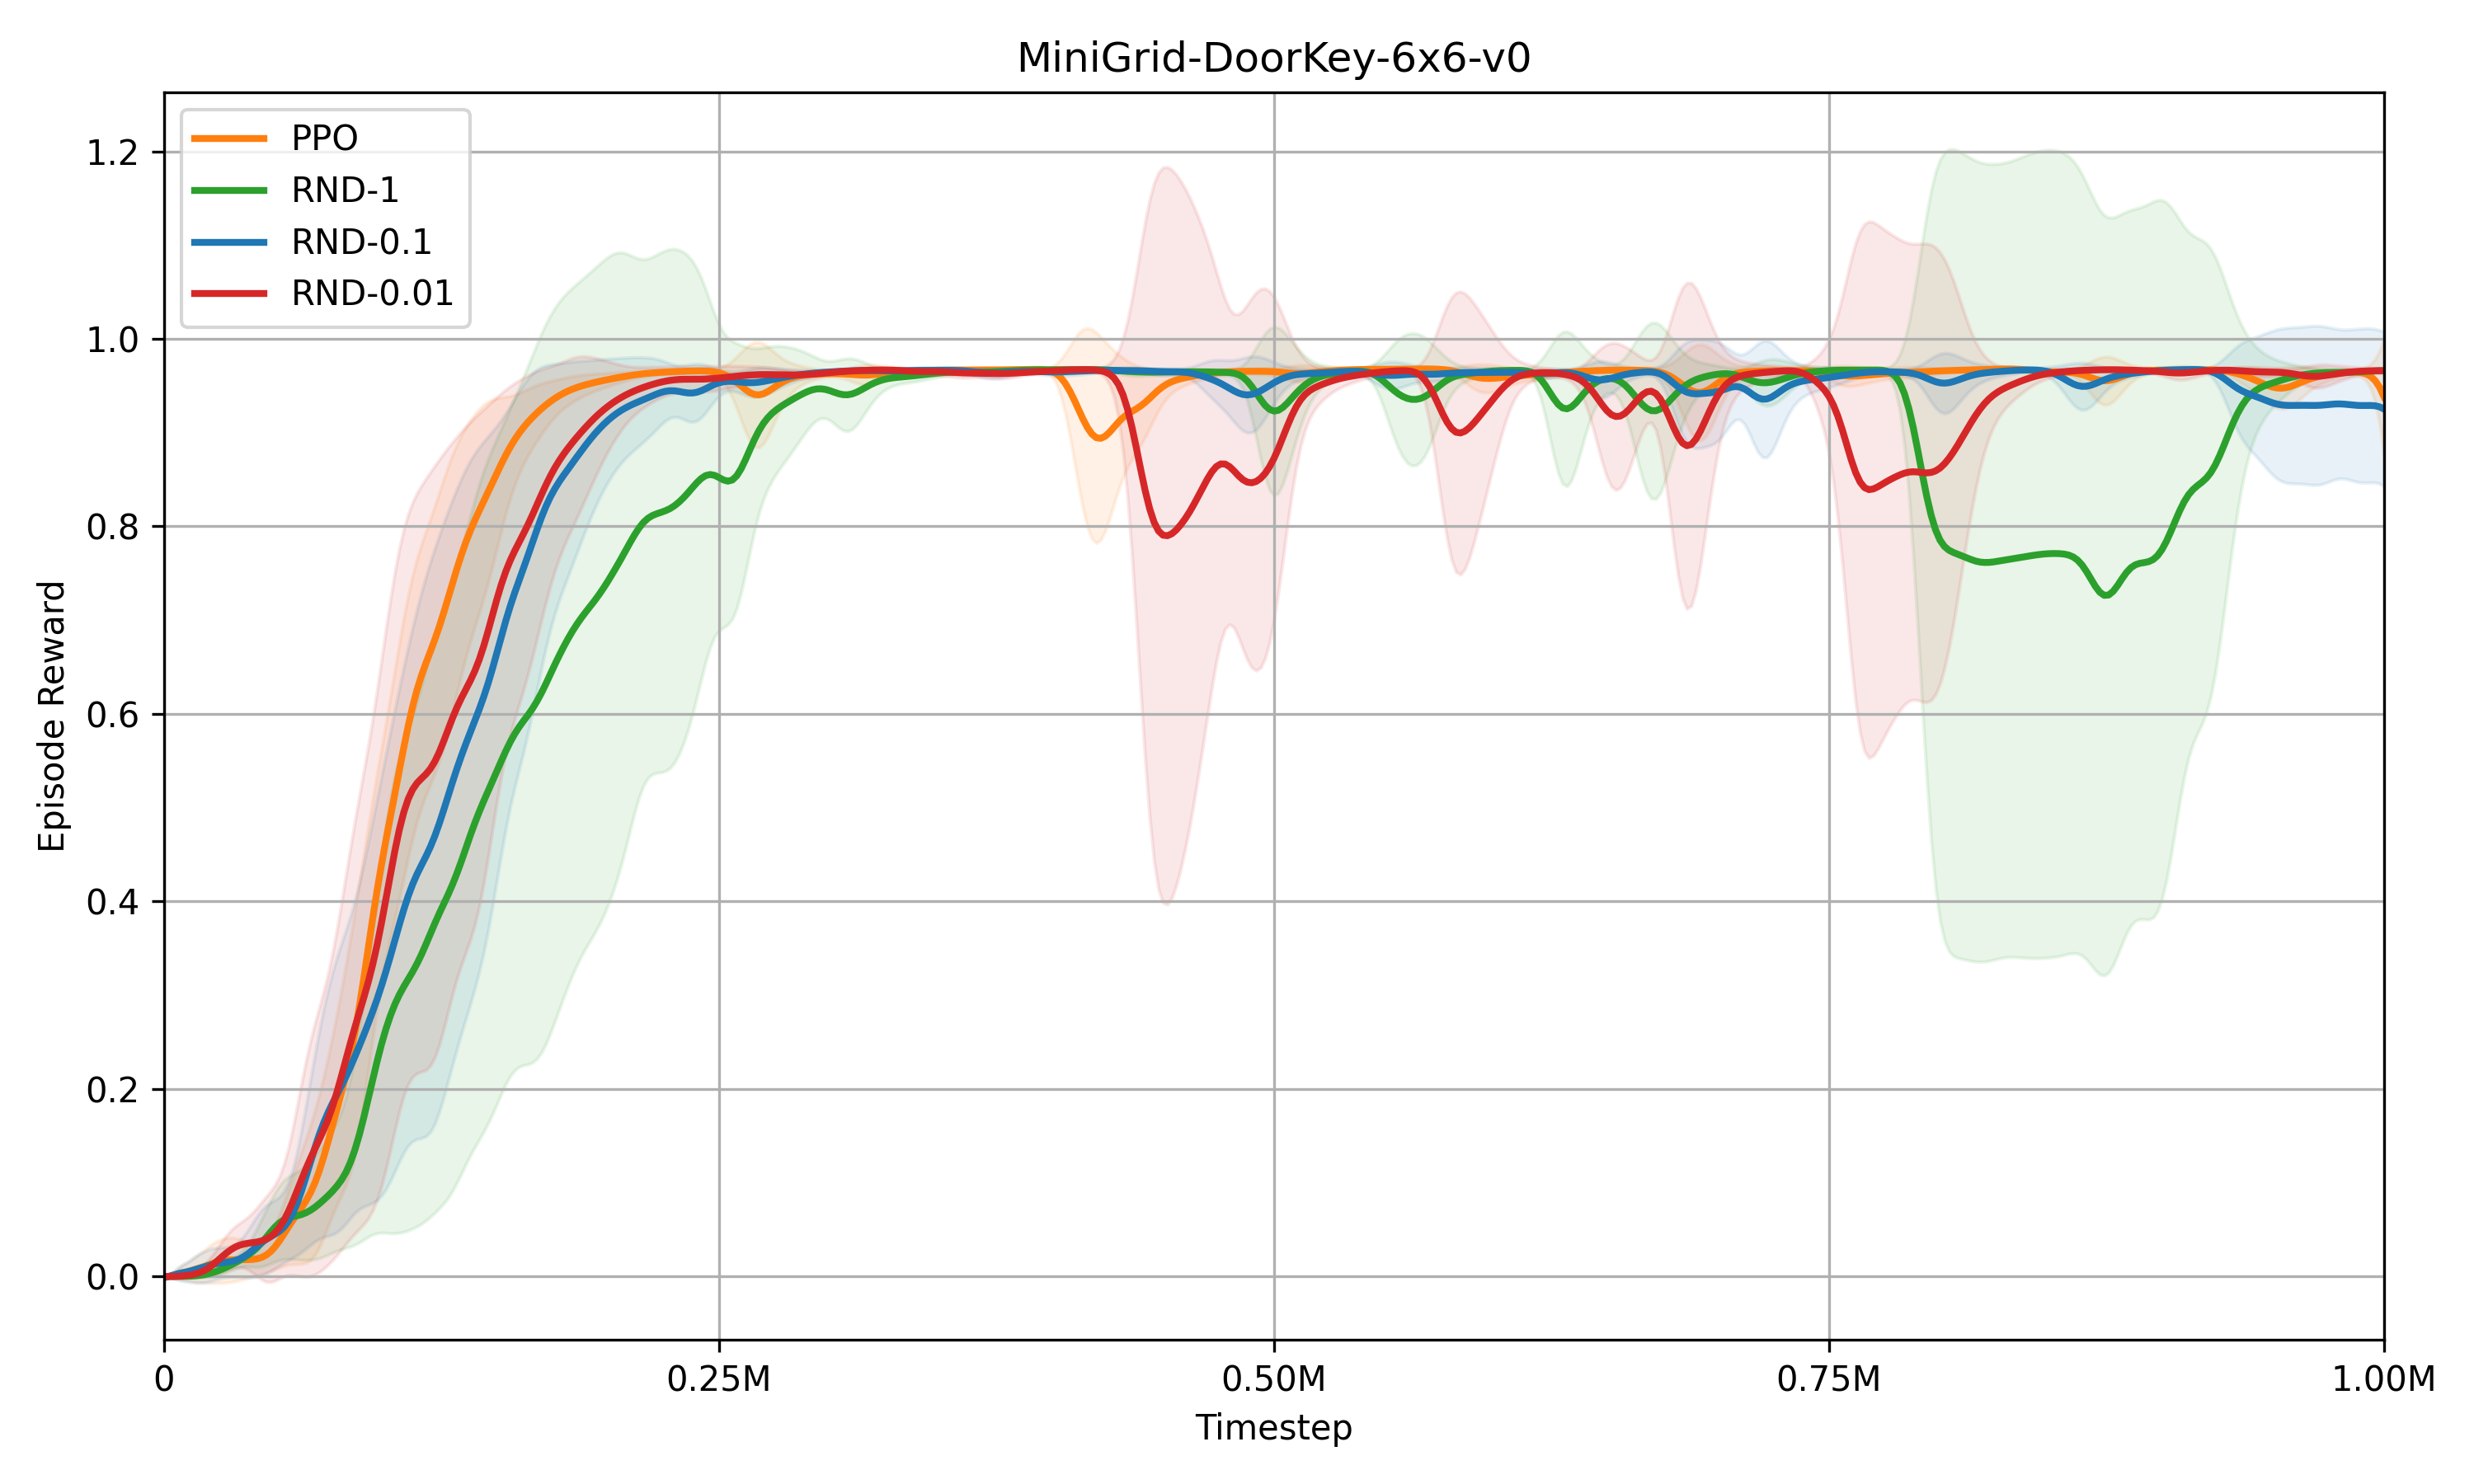
\includegraphics[width=\textwidth]{figs/MiniGrid-DoorKey-6x6-v0/episode_reward.png}
    
    (a) Episode Reward
\end{minipage}
\hfill
\begin{minipage}{0.45\textwidth}
    \centering
    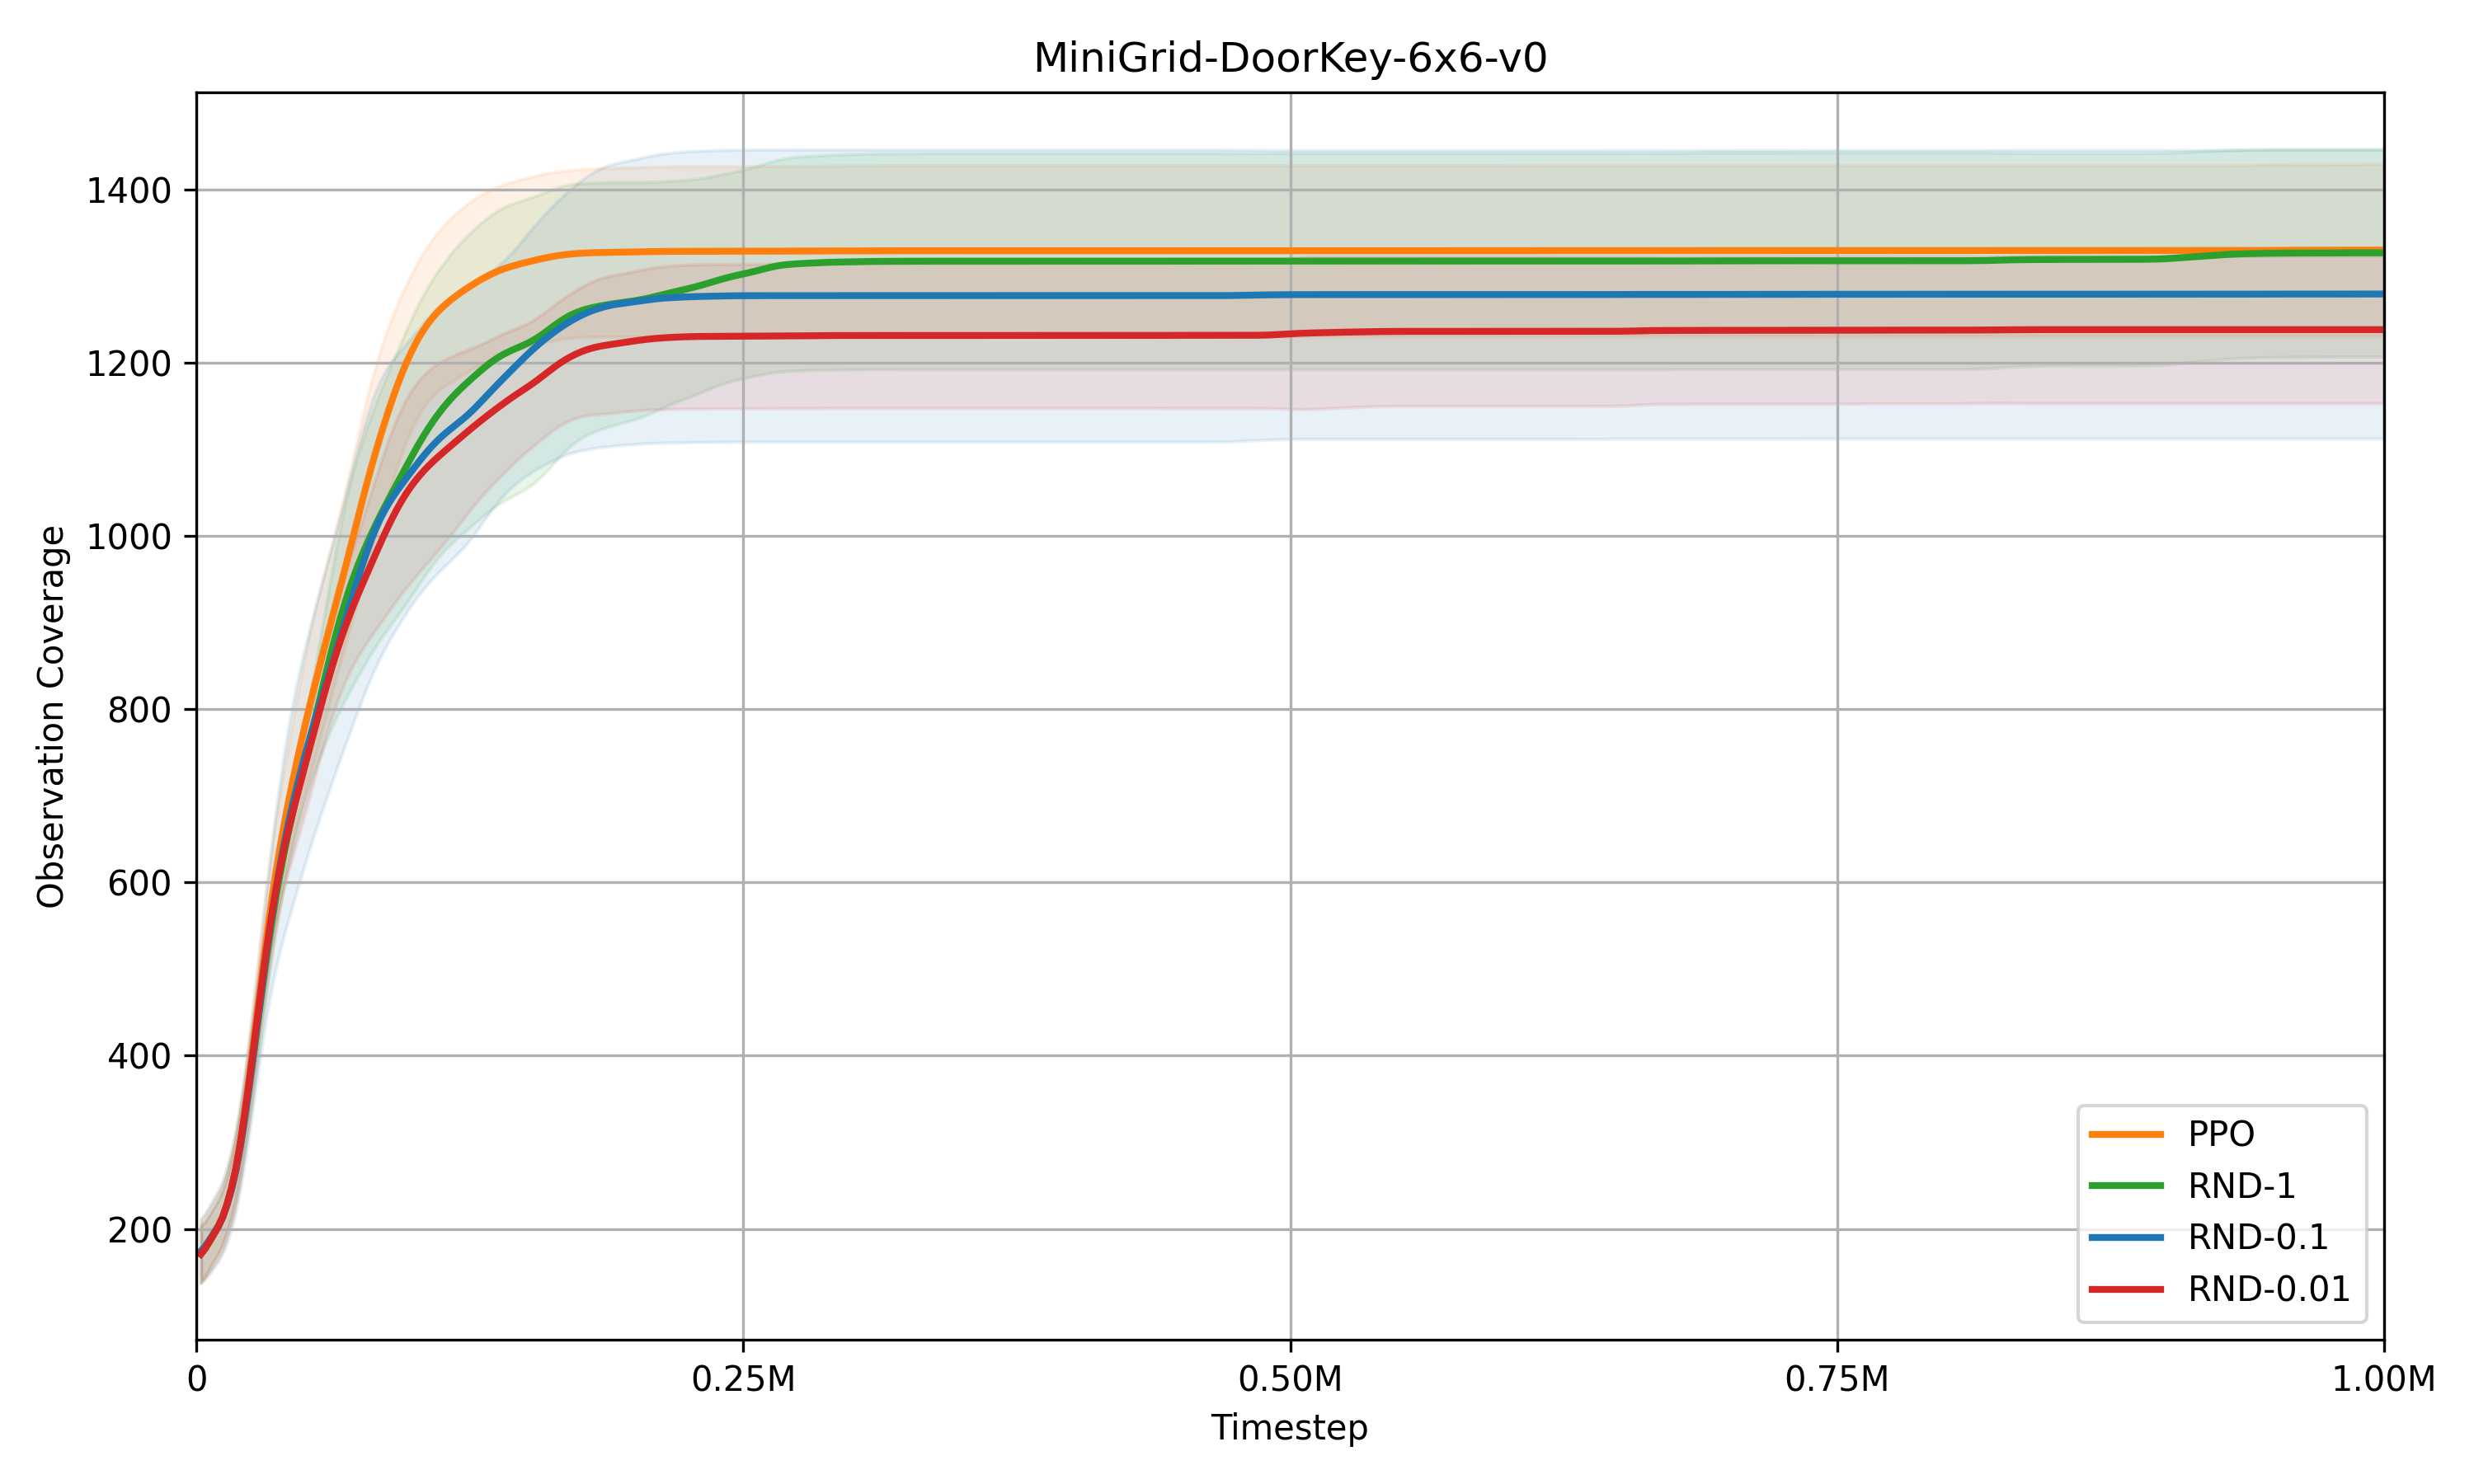
\includegraphics[width=\textwidth]{figs/MiniGrid-DoorKey-6x6-v0/obs_coverage.png}
    
    (b) Observation Coverage
\end{minipage}

\vspace{0.3cm}

\begin{minipage}{0.45\textwidth}
    \centering
    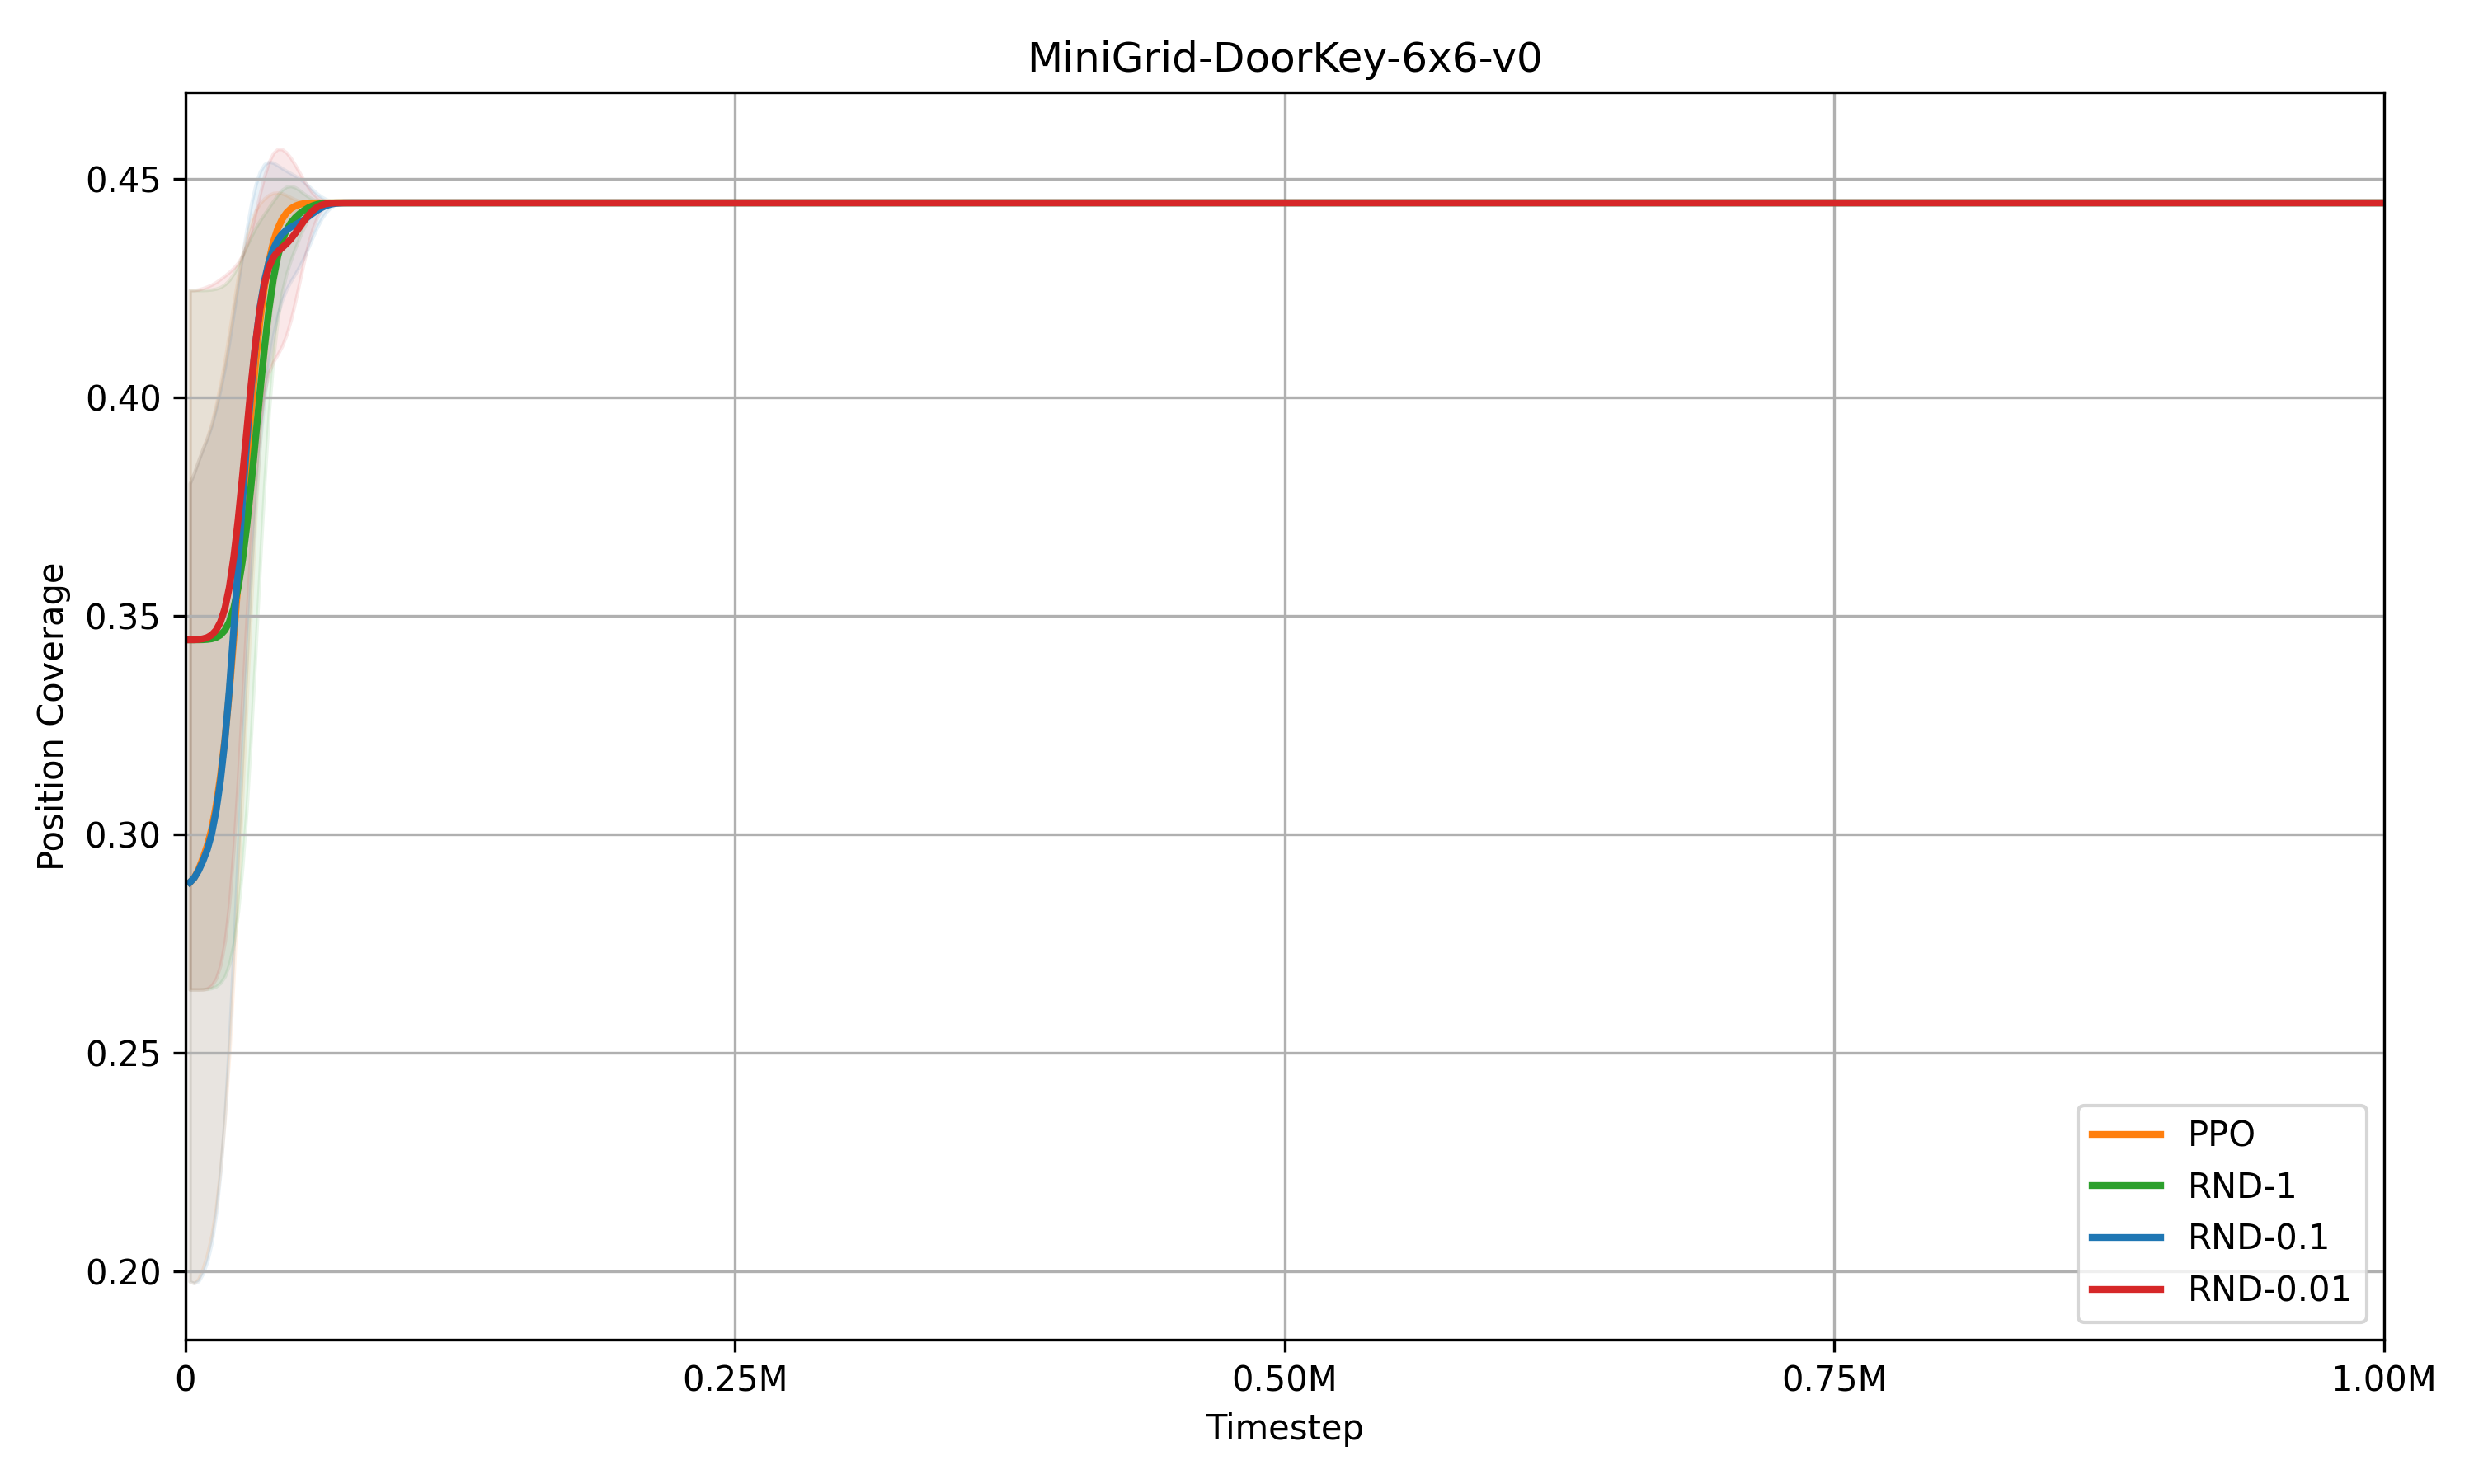
\includegraphics[width=\textwidth]{figs/MiniGrid-DoorKey-6x6-v0/pos_coverage.png}
    
    (c) Position Coverage
\end{minipage}
\hfill
\begin{minipage}{0.45\textwidth}
    \centering
    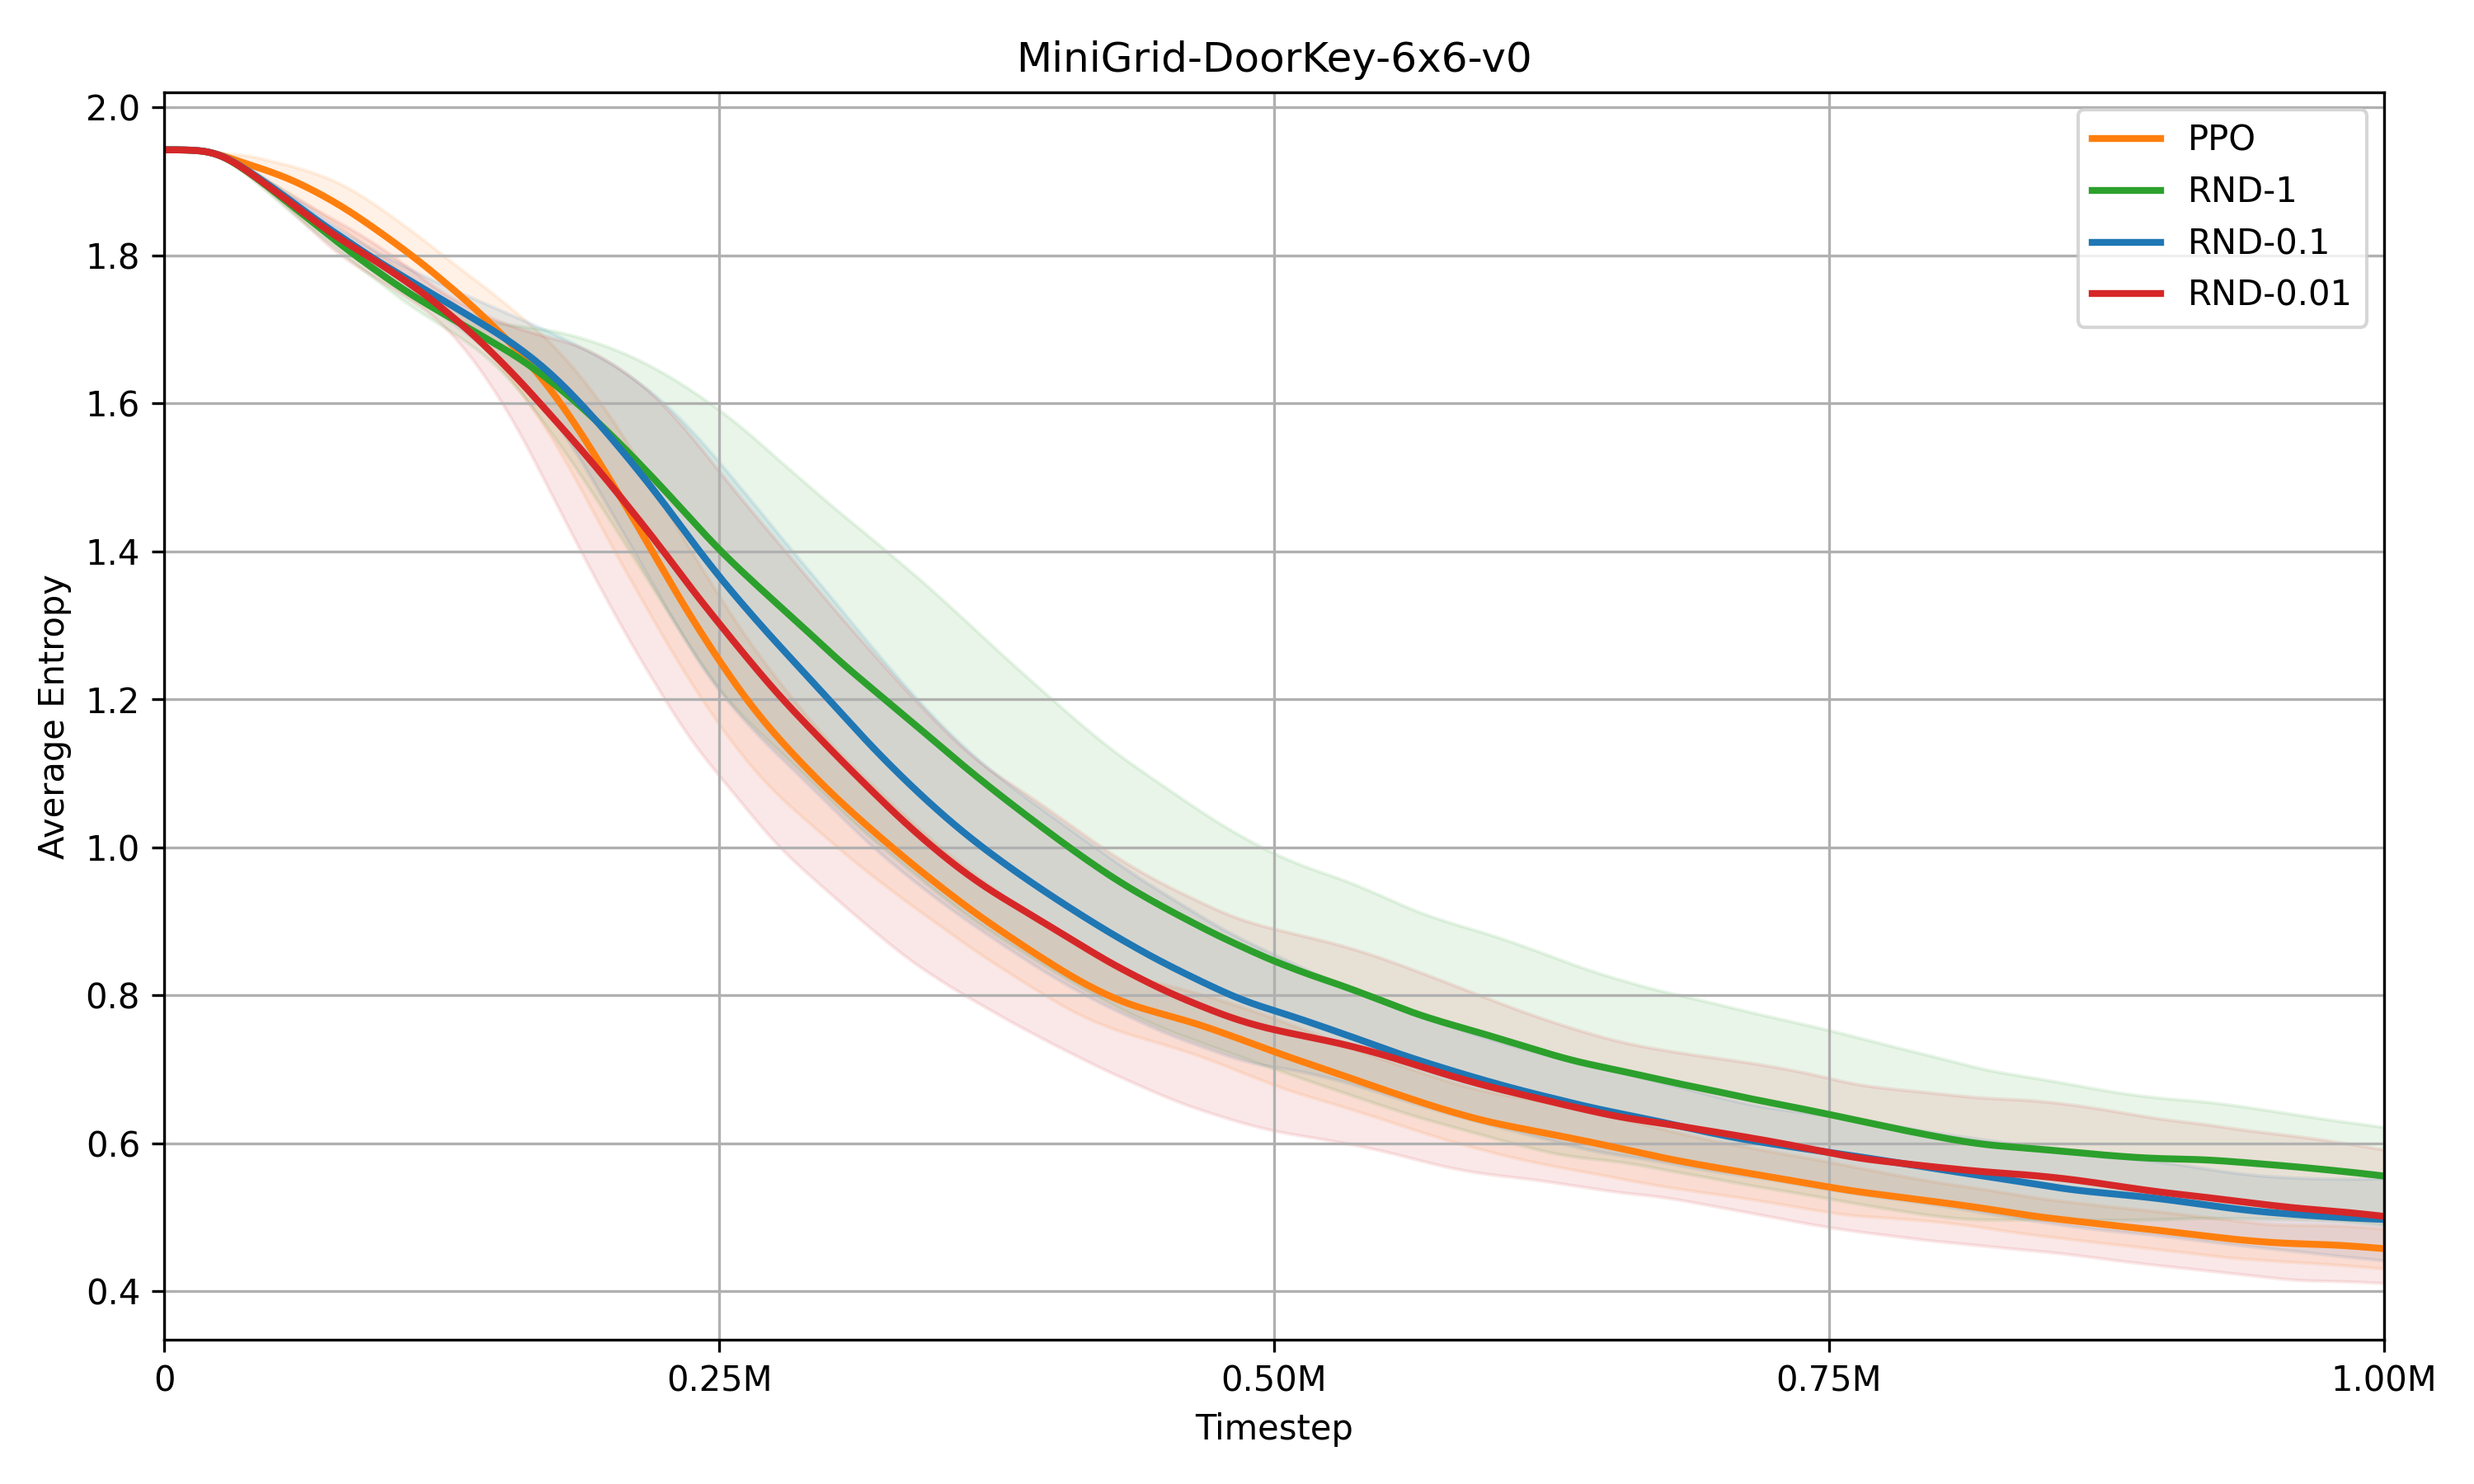
\includegraphics[width=\textwidth]{figs/MiniGrid-DoorKey-6x6-v0/avg_entropy.png}
    
    (d) Policy Entropy
\end{minipage}
\end{figure}

\begin{figure}[H]{Các chỉ số huấn luyện trên DoorKey-8x8}
\centering
\begin{minipage}{0.45\textwidth}
    \centering
    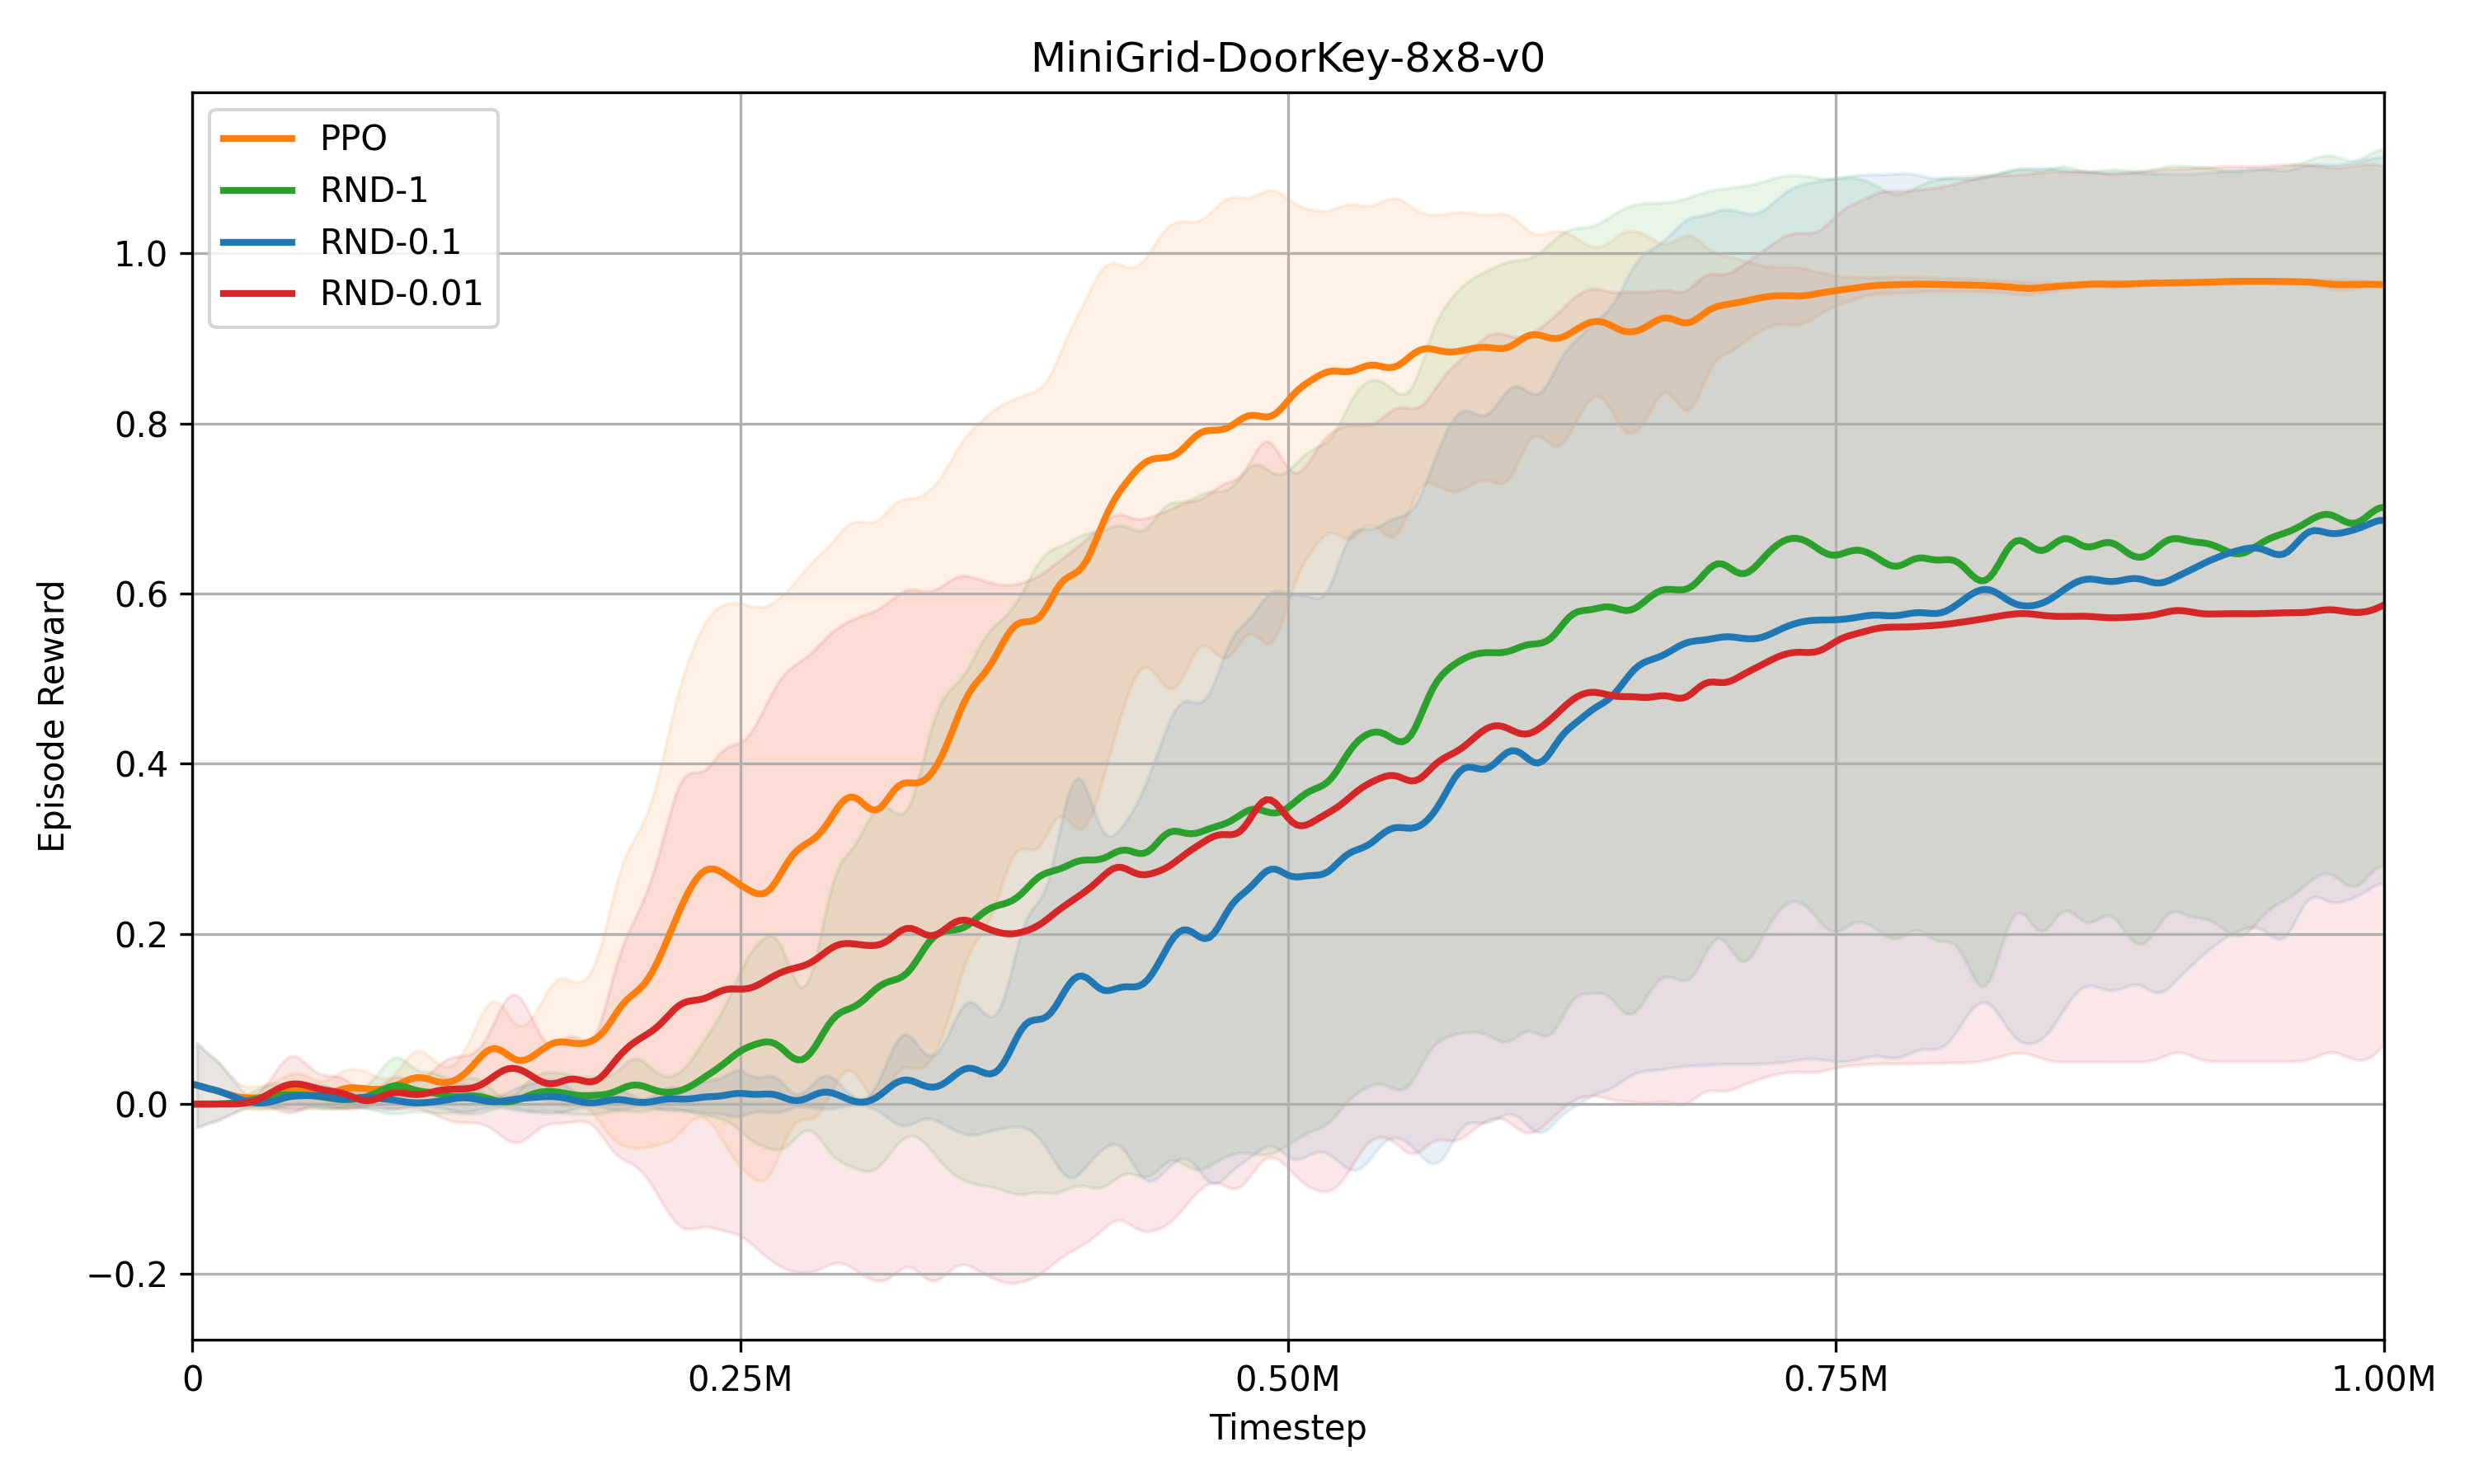
\includegraphics[width=\textwidth]{figs/MiniGrid-DoorKey-8x8-v0/episode_reward.png}
    
    (a) Episode Reward
\end{minipage}
\hfill
\begin{minipage}{0.45\textwidth}
    \centering
    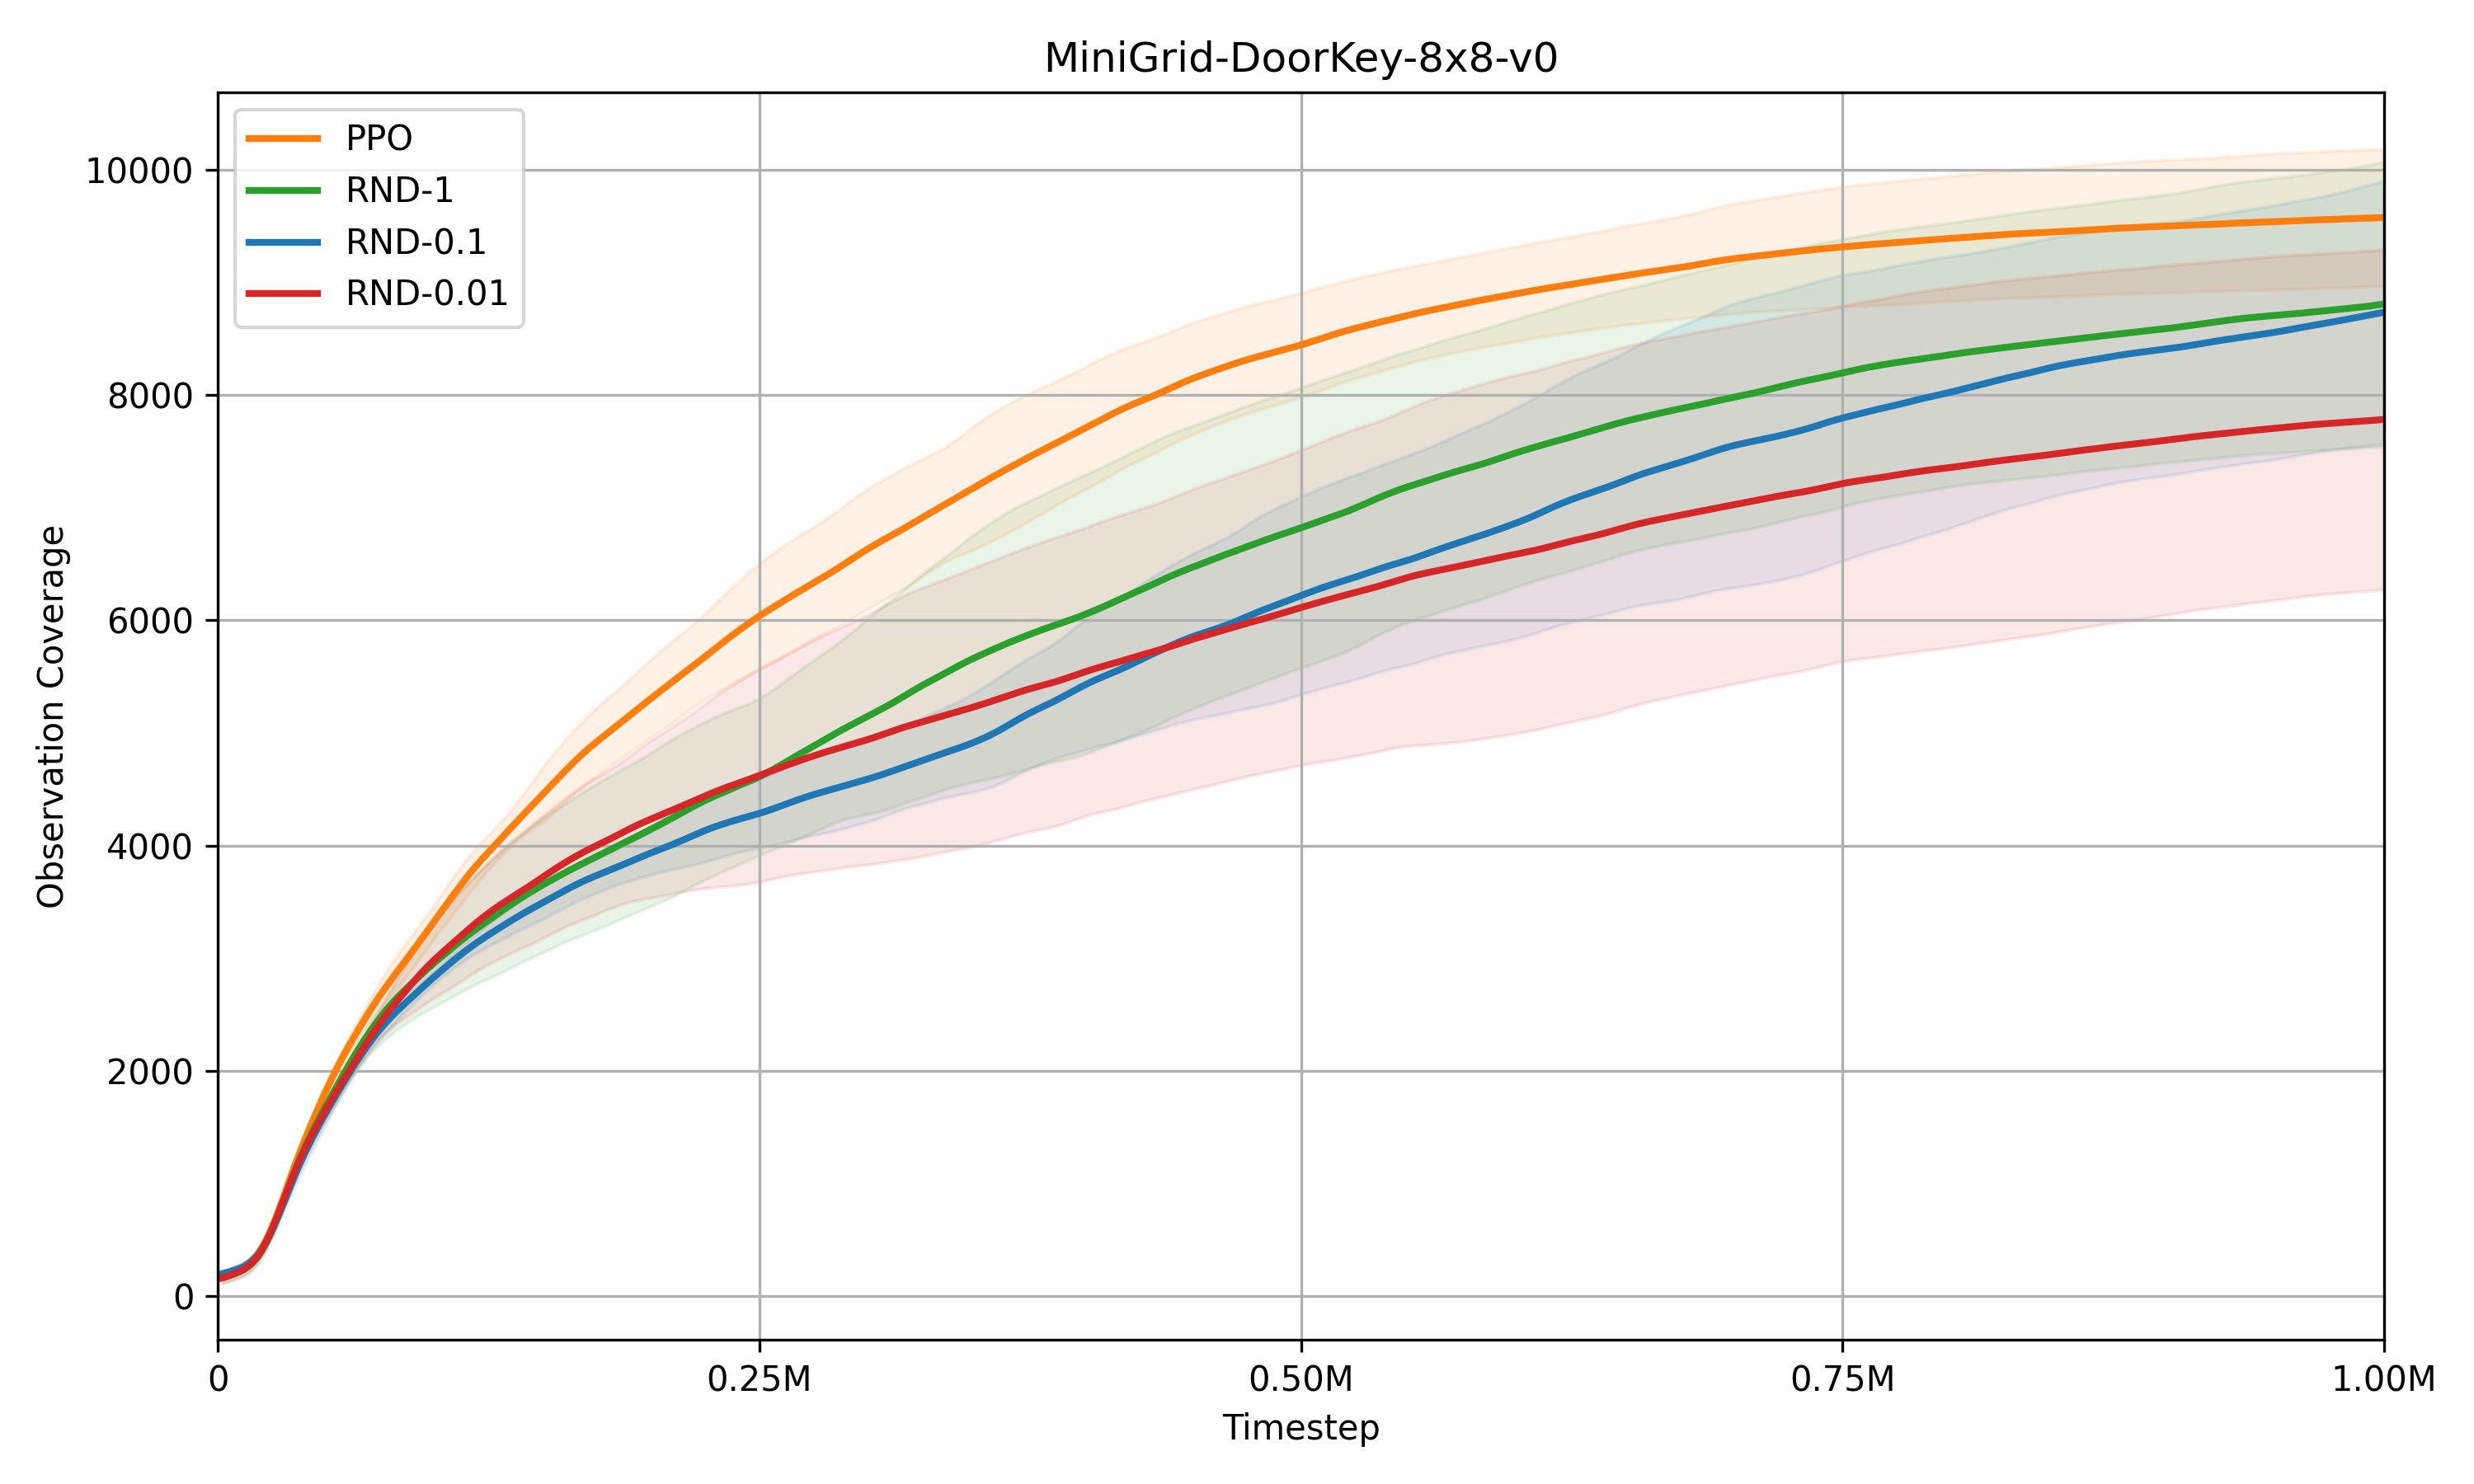
\includegraphics[width=\textwidth]{figs/MiniGrid-DoorKey-8x8-v0/obs_coverage.png}
    
    (b) Observation Coverage
\end{minipage}

\vspace{0.3cm}

\begin{minipage}{0.45\textwidth}
    \centering
    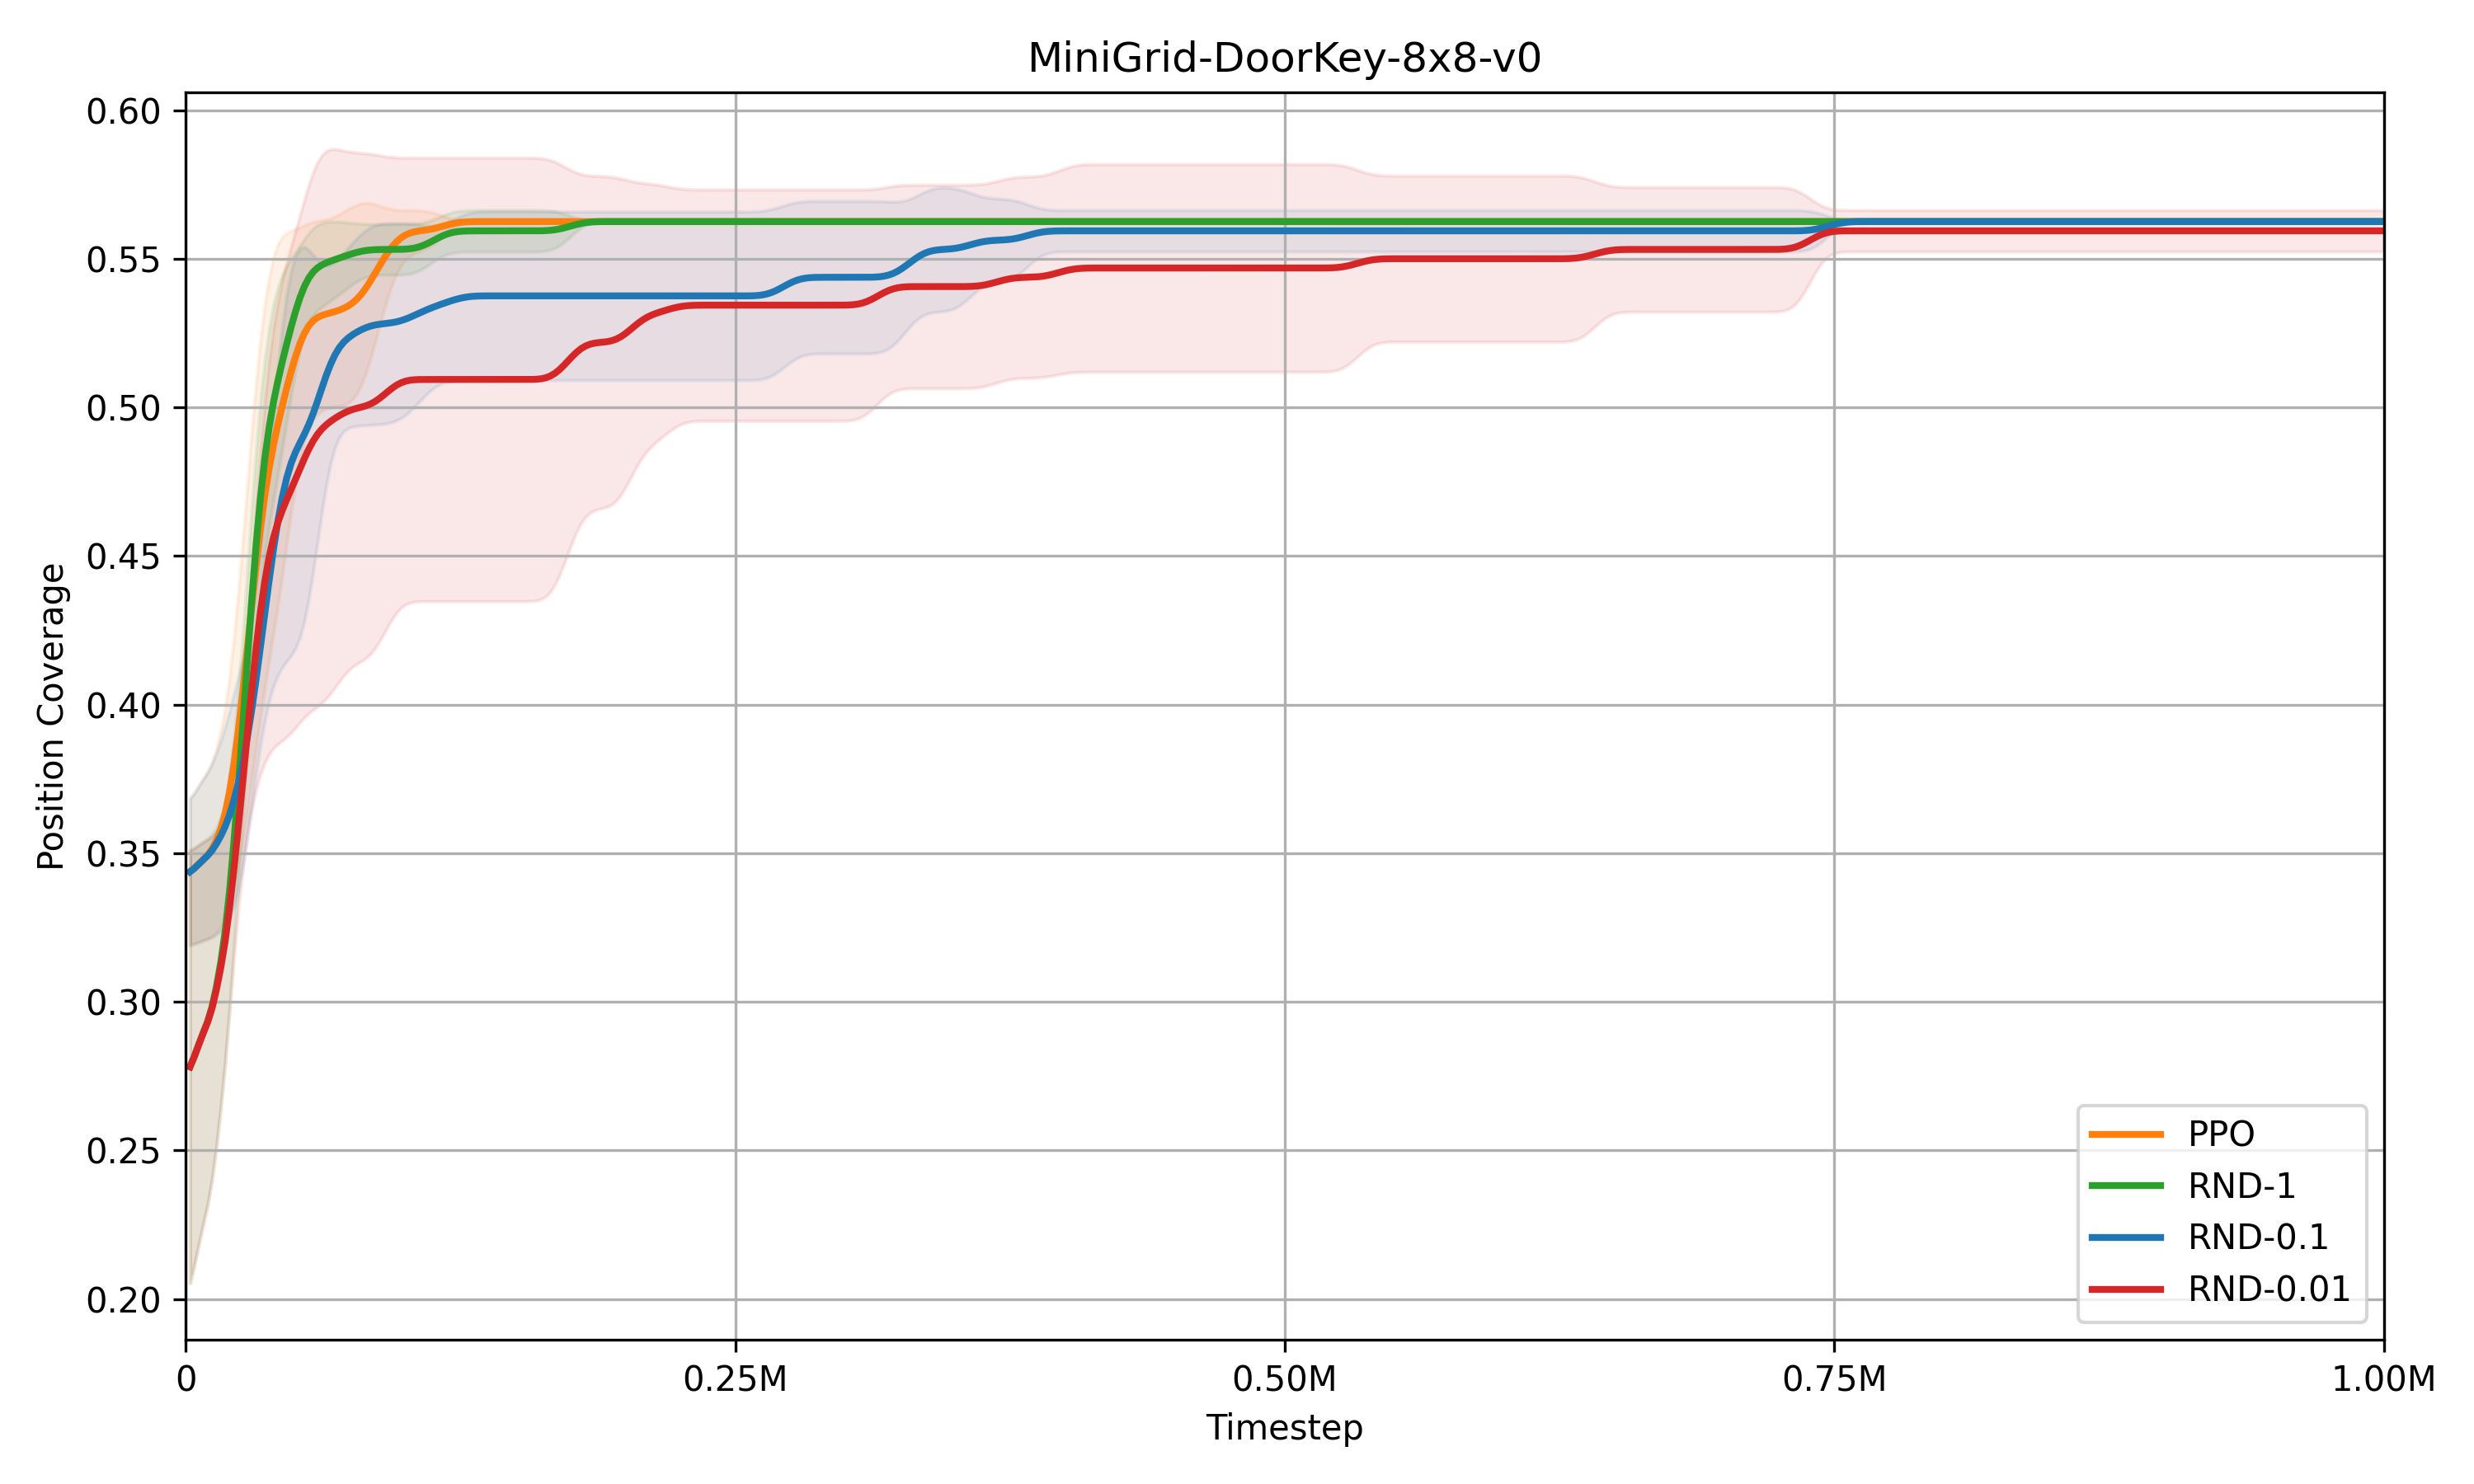
\includegraphics[width=\textwidth]{figs/MiniGrid-DoorKey-8x8-v0/pos_coverage.png}
    
    (c) Position Coverage
\end{minipage}
\hfill
\begin{minipage}{0.45\textwidth}
    \centering
    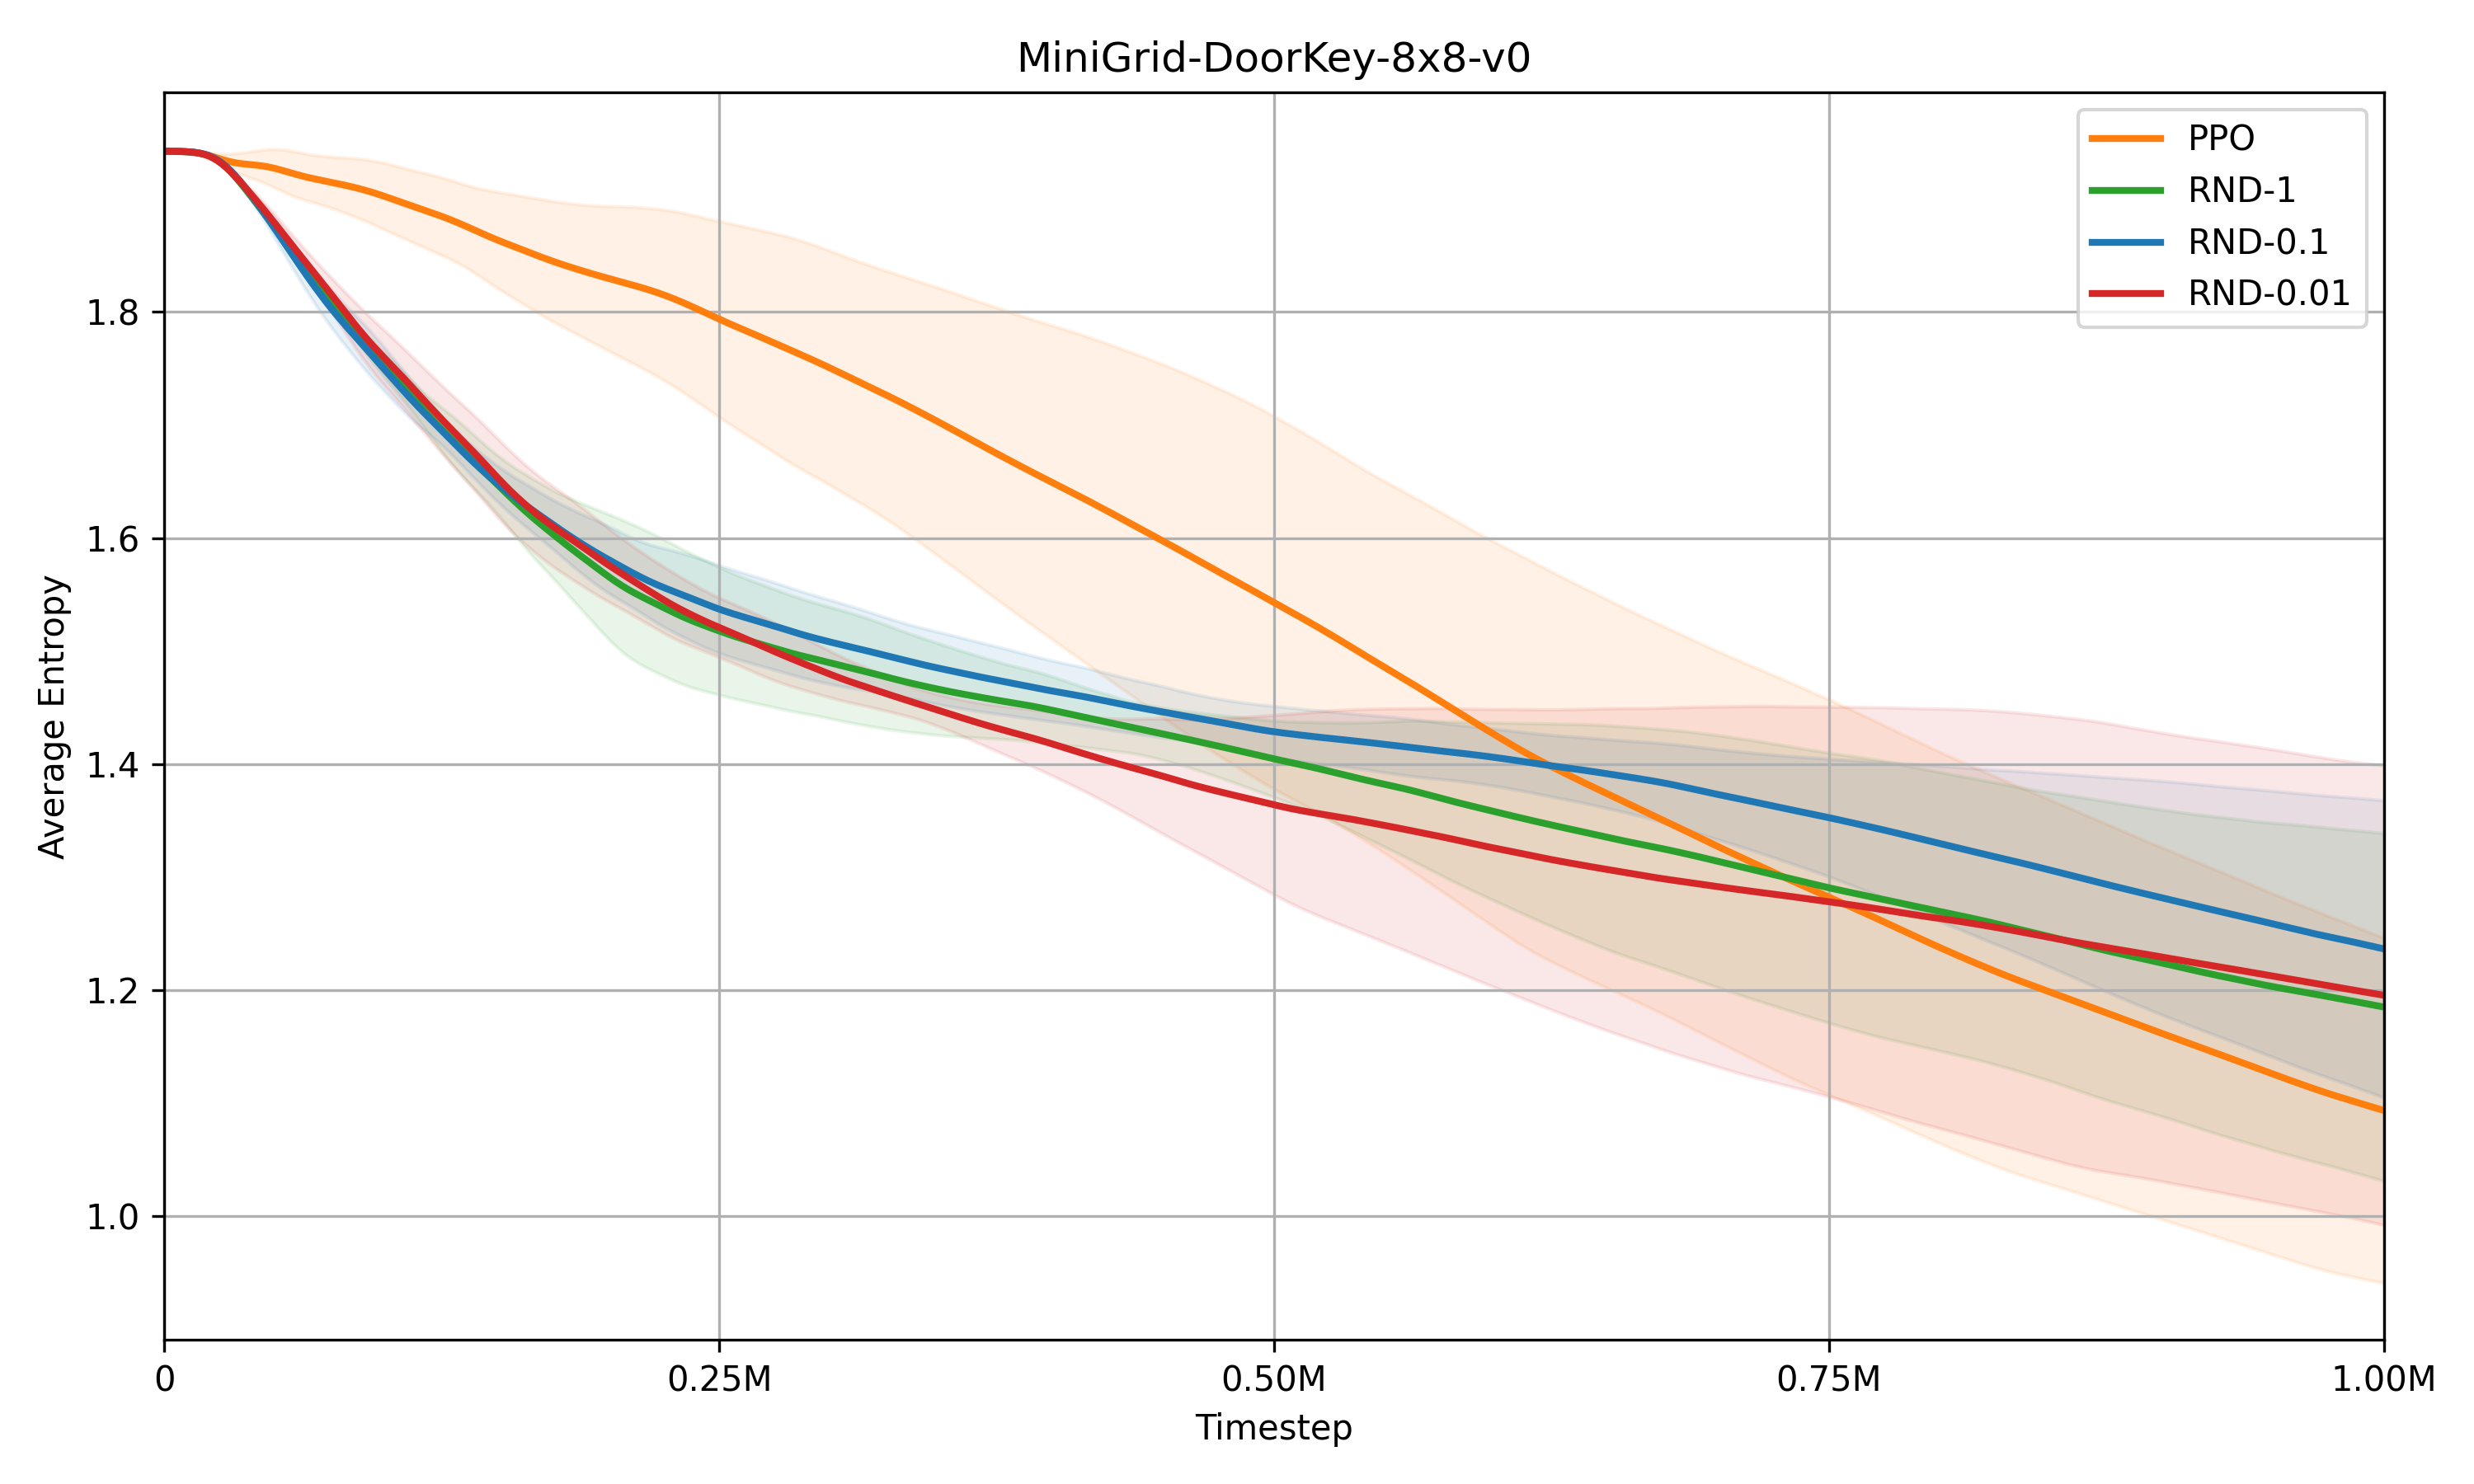
\includegraphics[width=\textwidth]{figs/MiniGrid-DoorKey-8x8-v0/avg_entropy.png}
    
    (d) Policy Entropy
\end{minipage}
\end{figure}

\subsection{Kết quả của RQ3}

\begin{figure}[H]{Các chỉ số huấn luyện trên KeyCorridor-S3R1}
\centering
\begin{minipage}{0.45\textwidth}
    \centering
    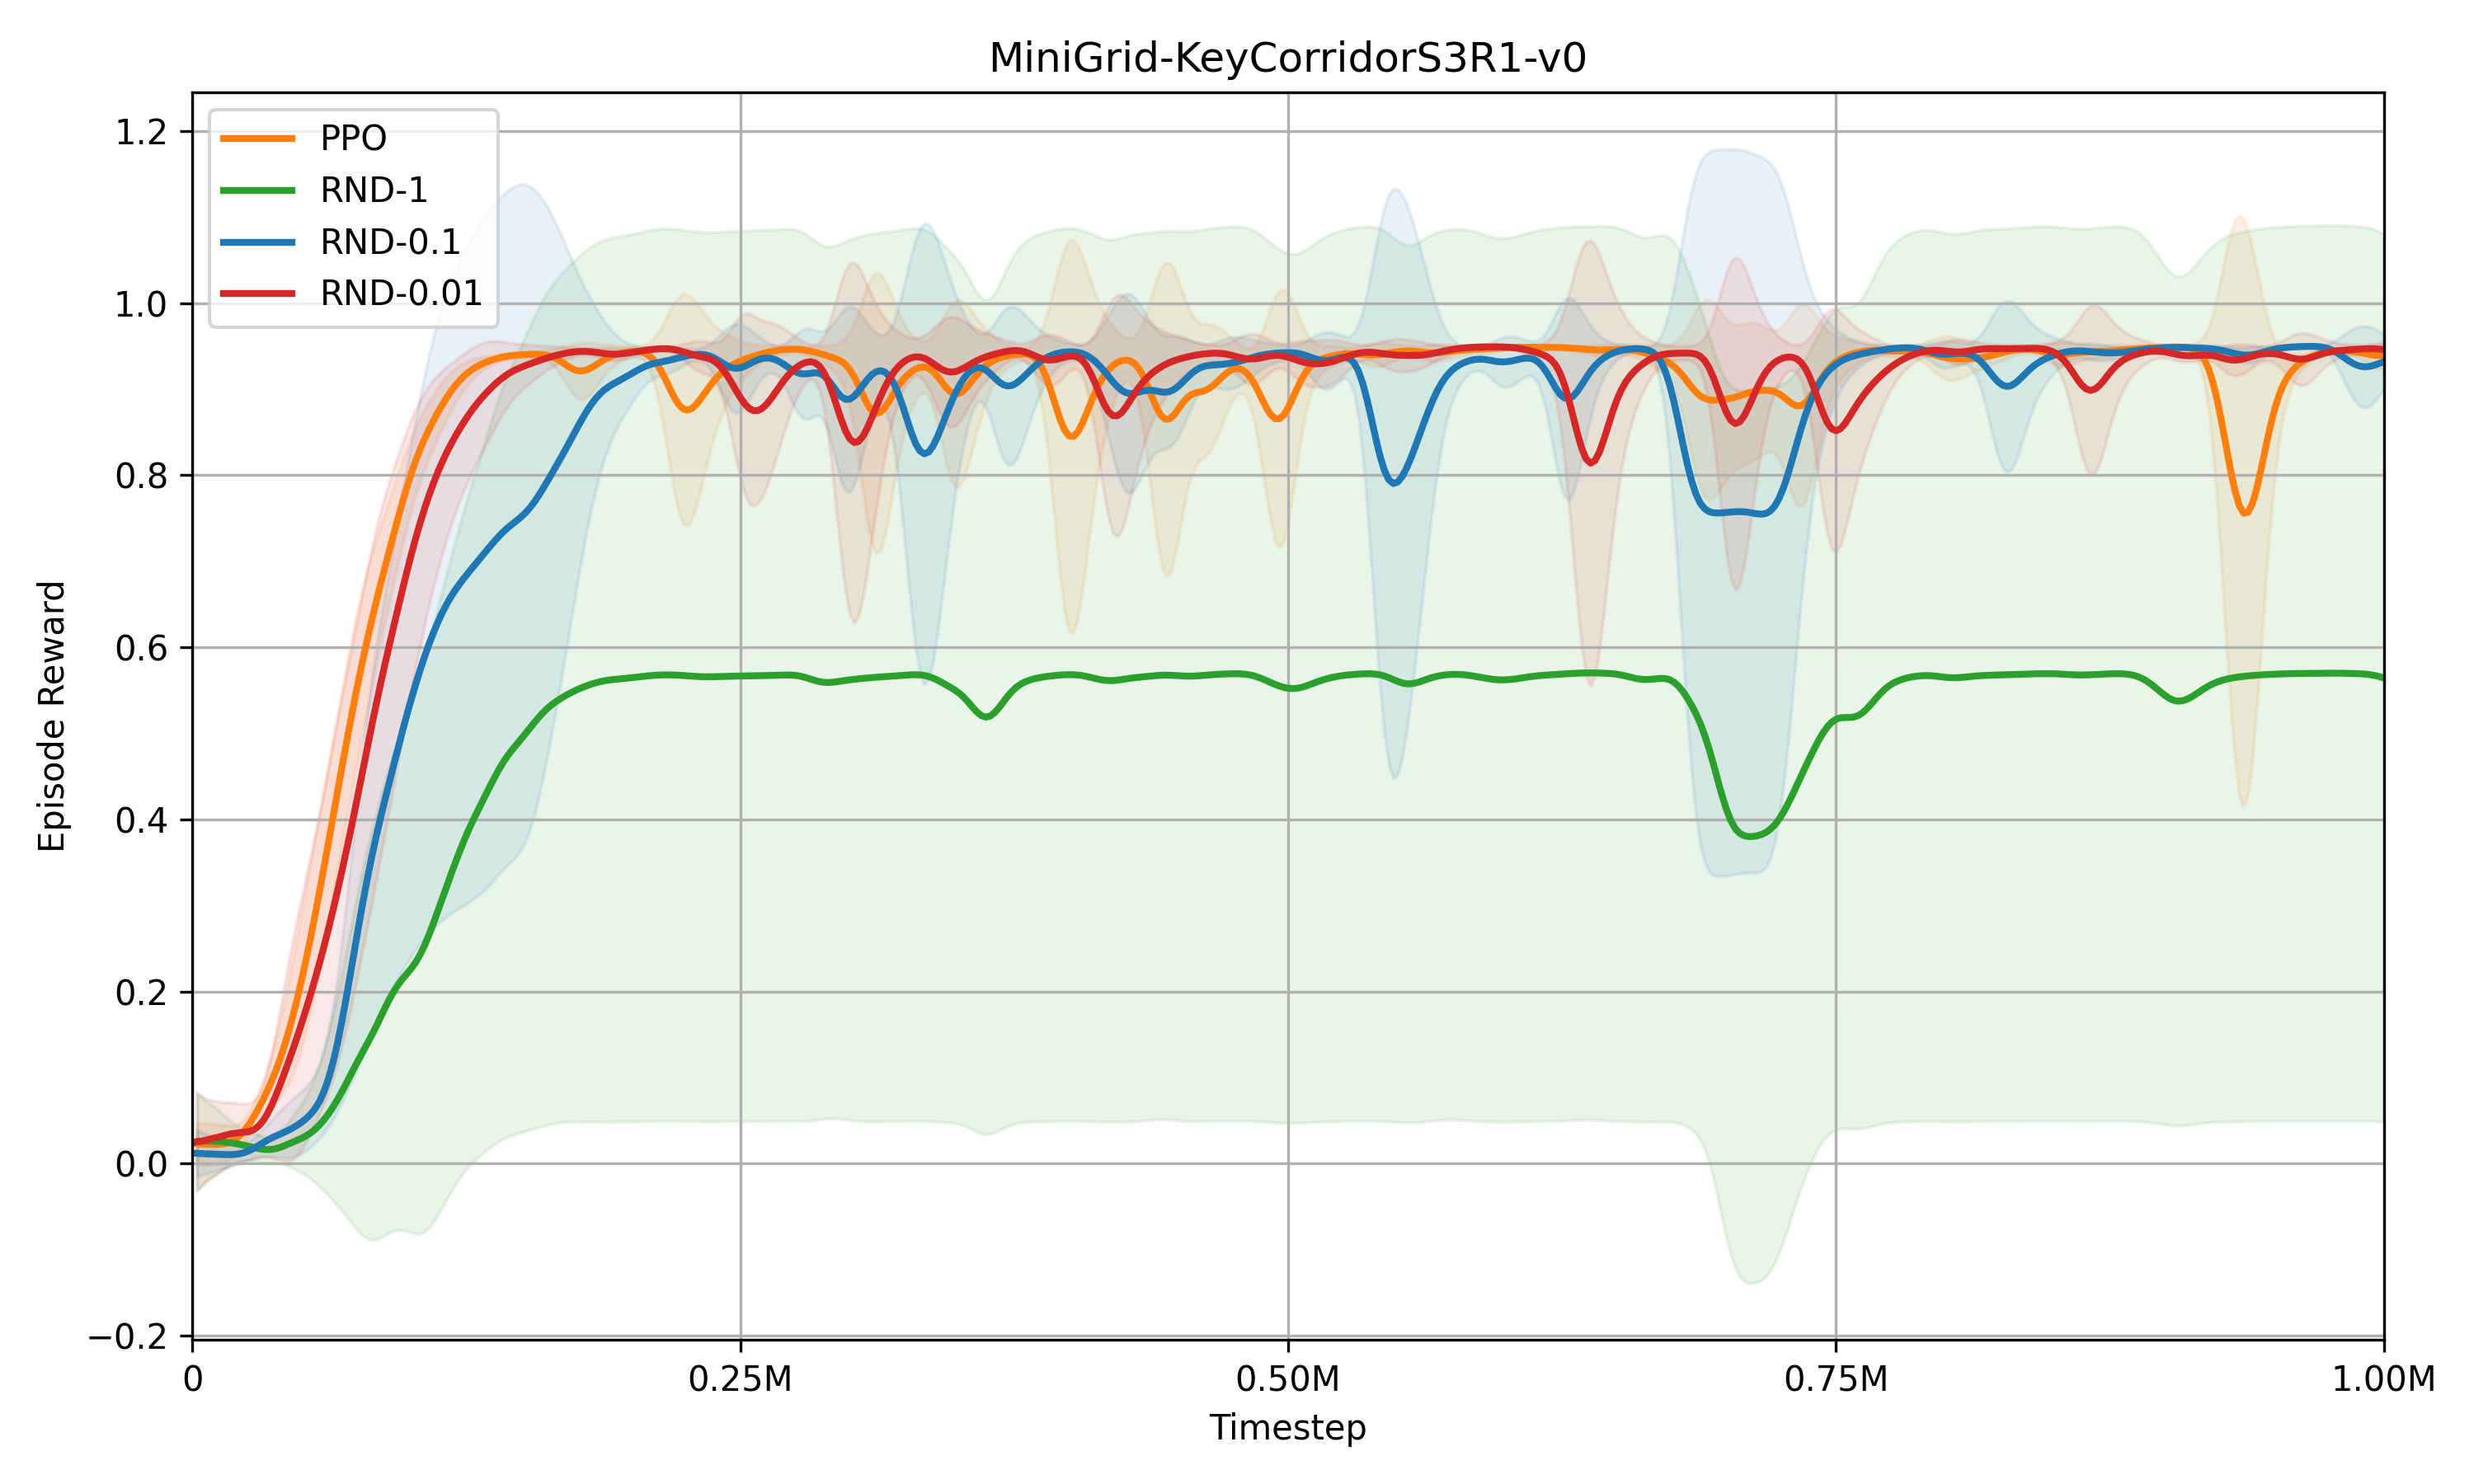
\includegraphics[width=\textwidth]{figs/MiniGrid-KeyCorridorS3R1-v0/episode_reward.png}
    
    (a) Episode Reward
\end{minipage}
\hfill
\begin{minipage}{0.45\textwidth}
    \centering
    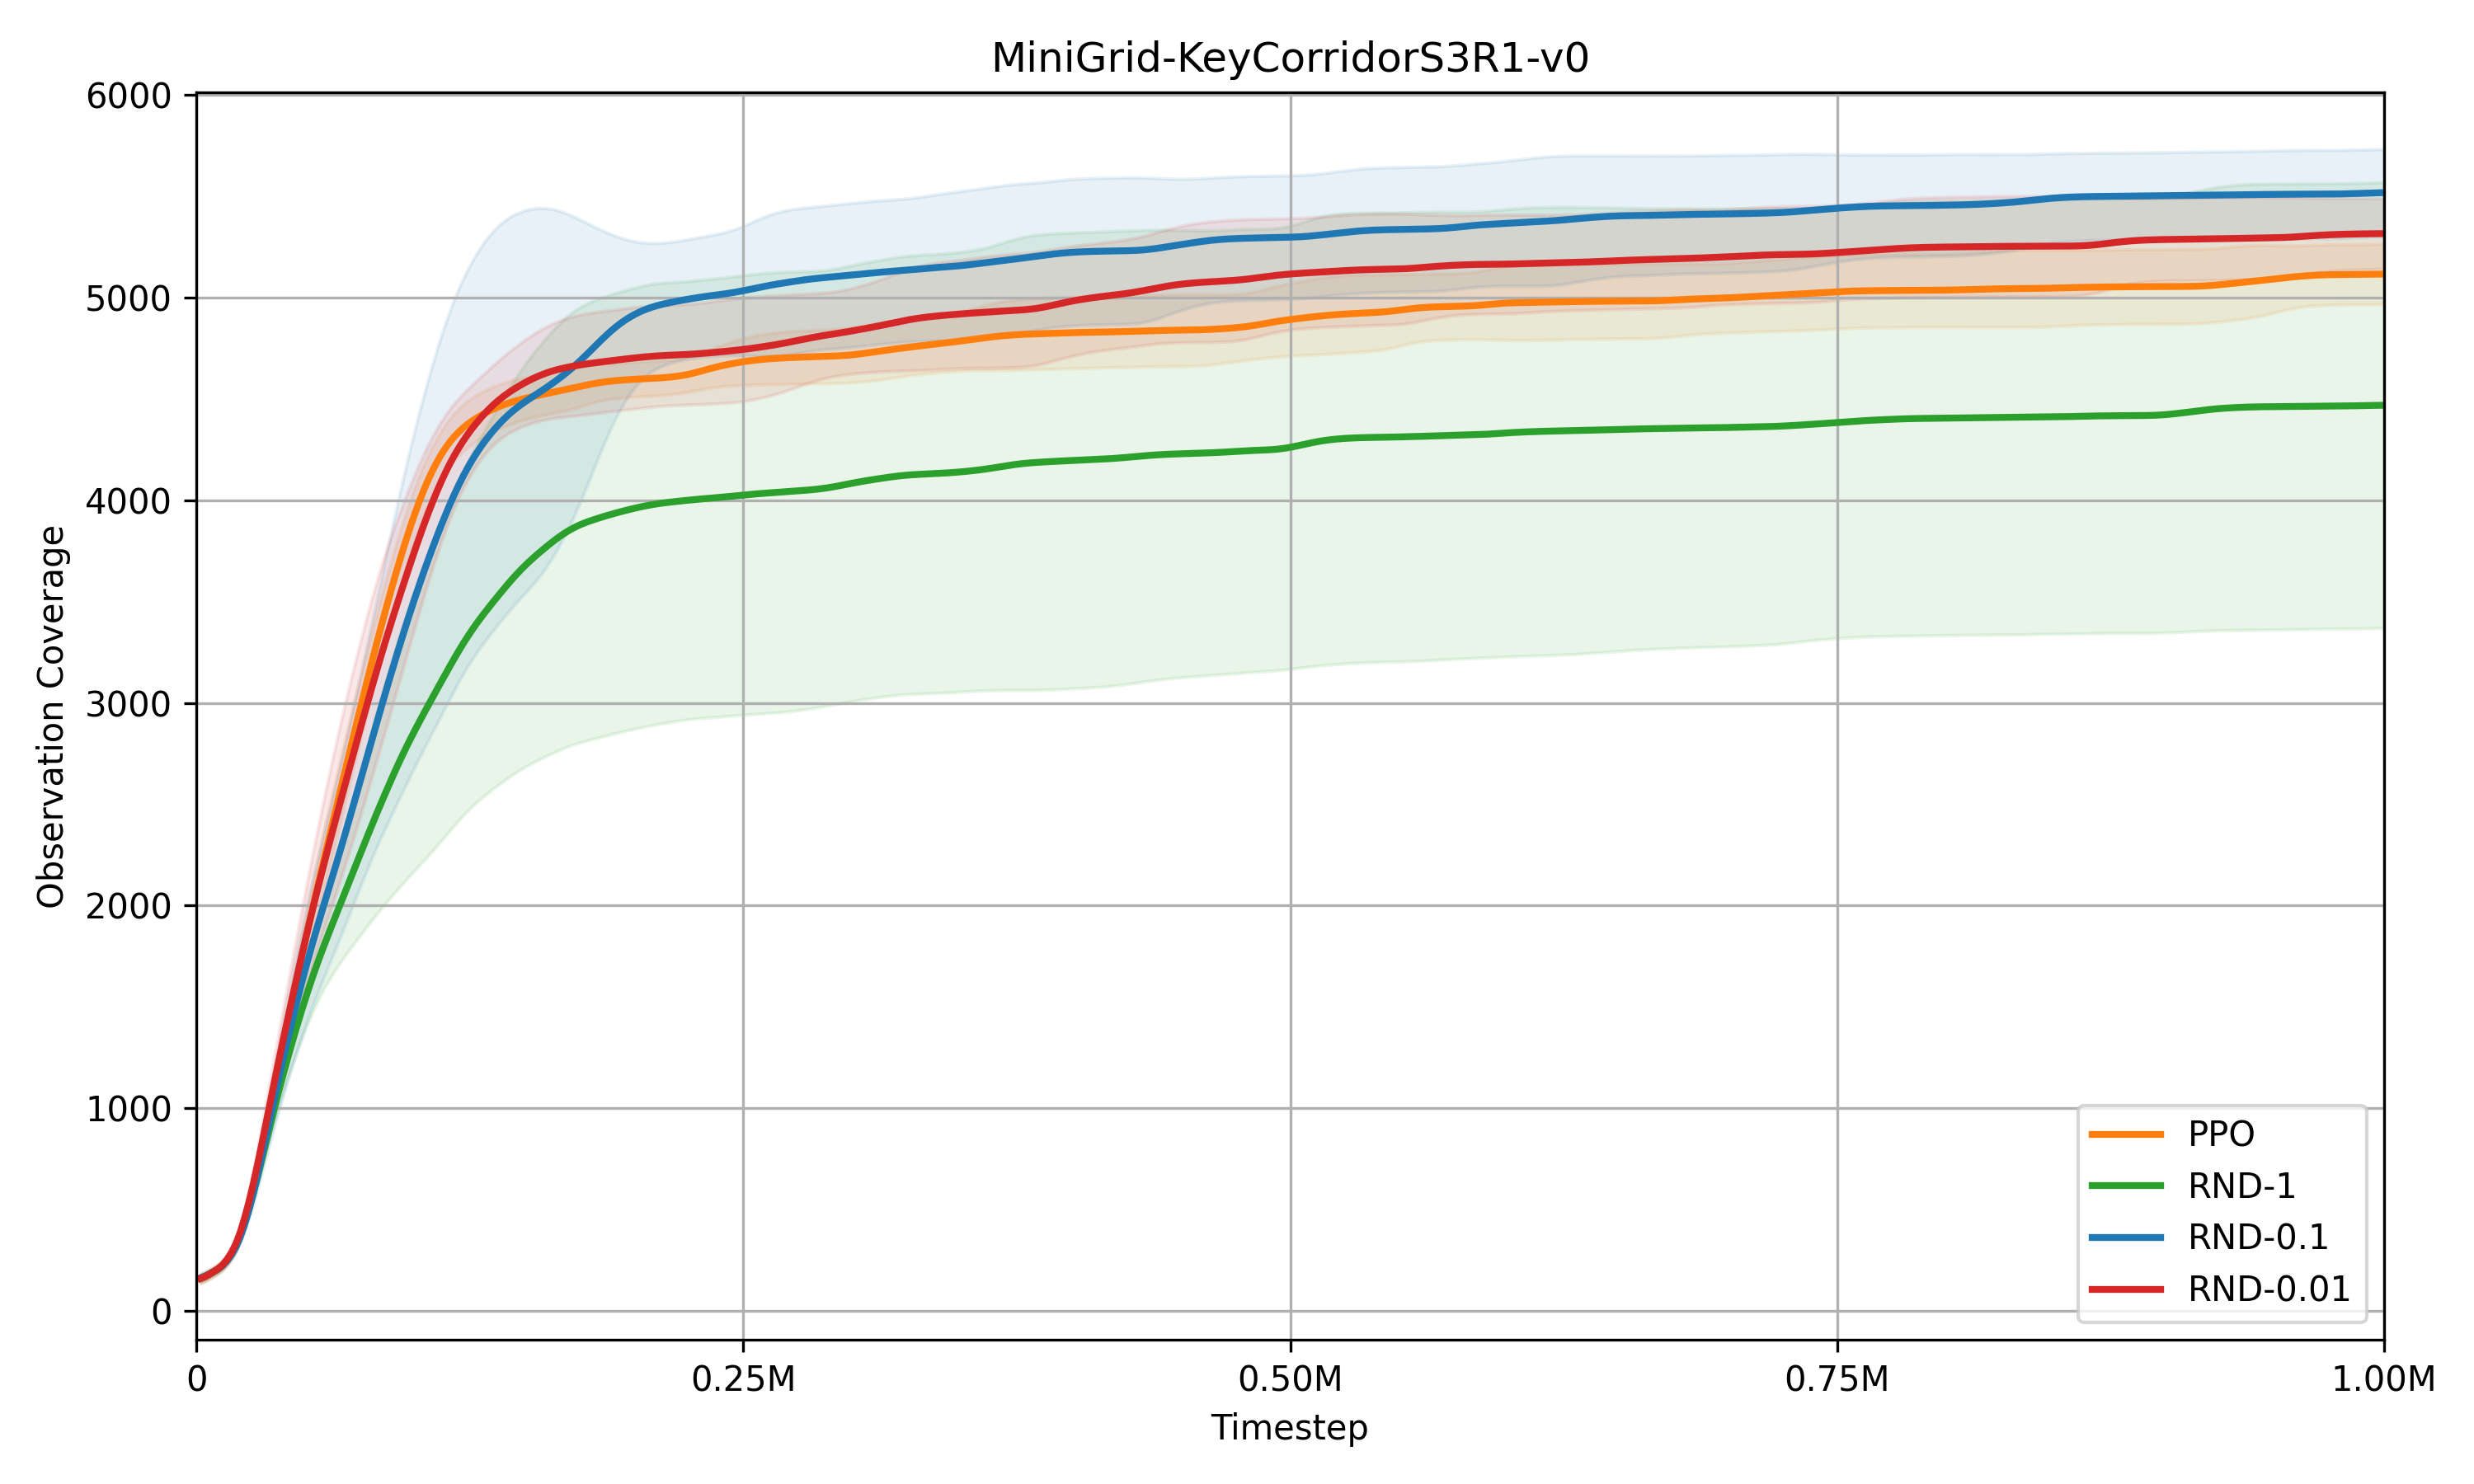
\includegraphics[width=\textwidth]{figs/MiniGrid-KeyCorridorS3R1-v0/obs_coverage.png}
    
    (b) Observation Coverage
\end{minipage}

\vspace{0.3cm}

\begin{minipage}{0.45\textwidth}
    \centering
    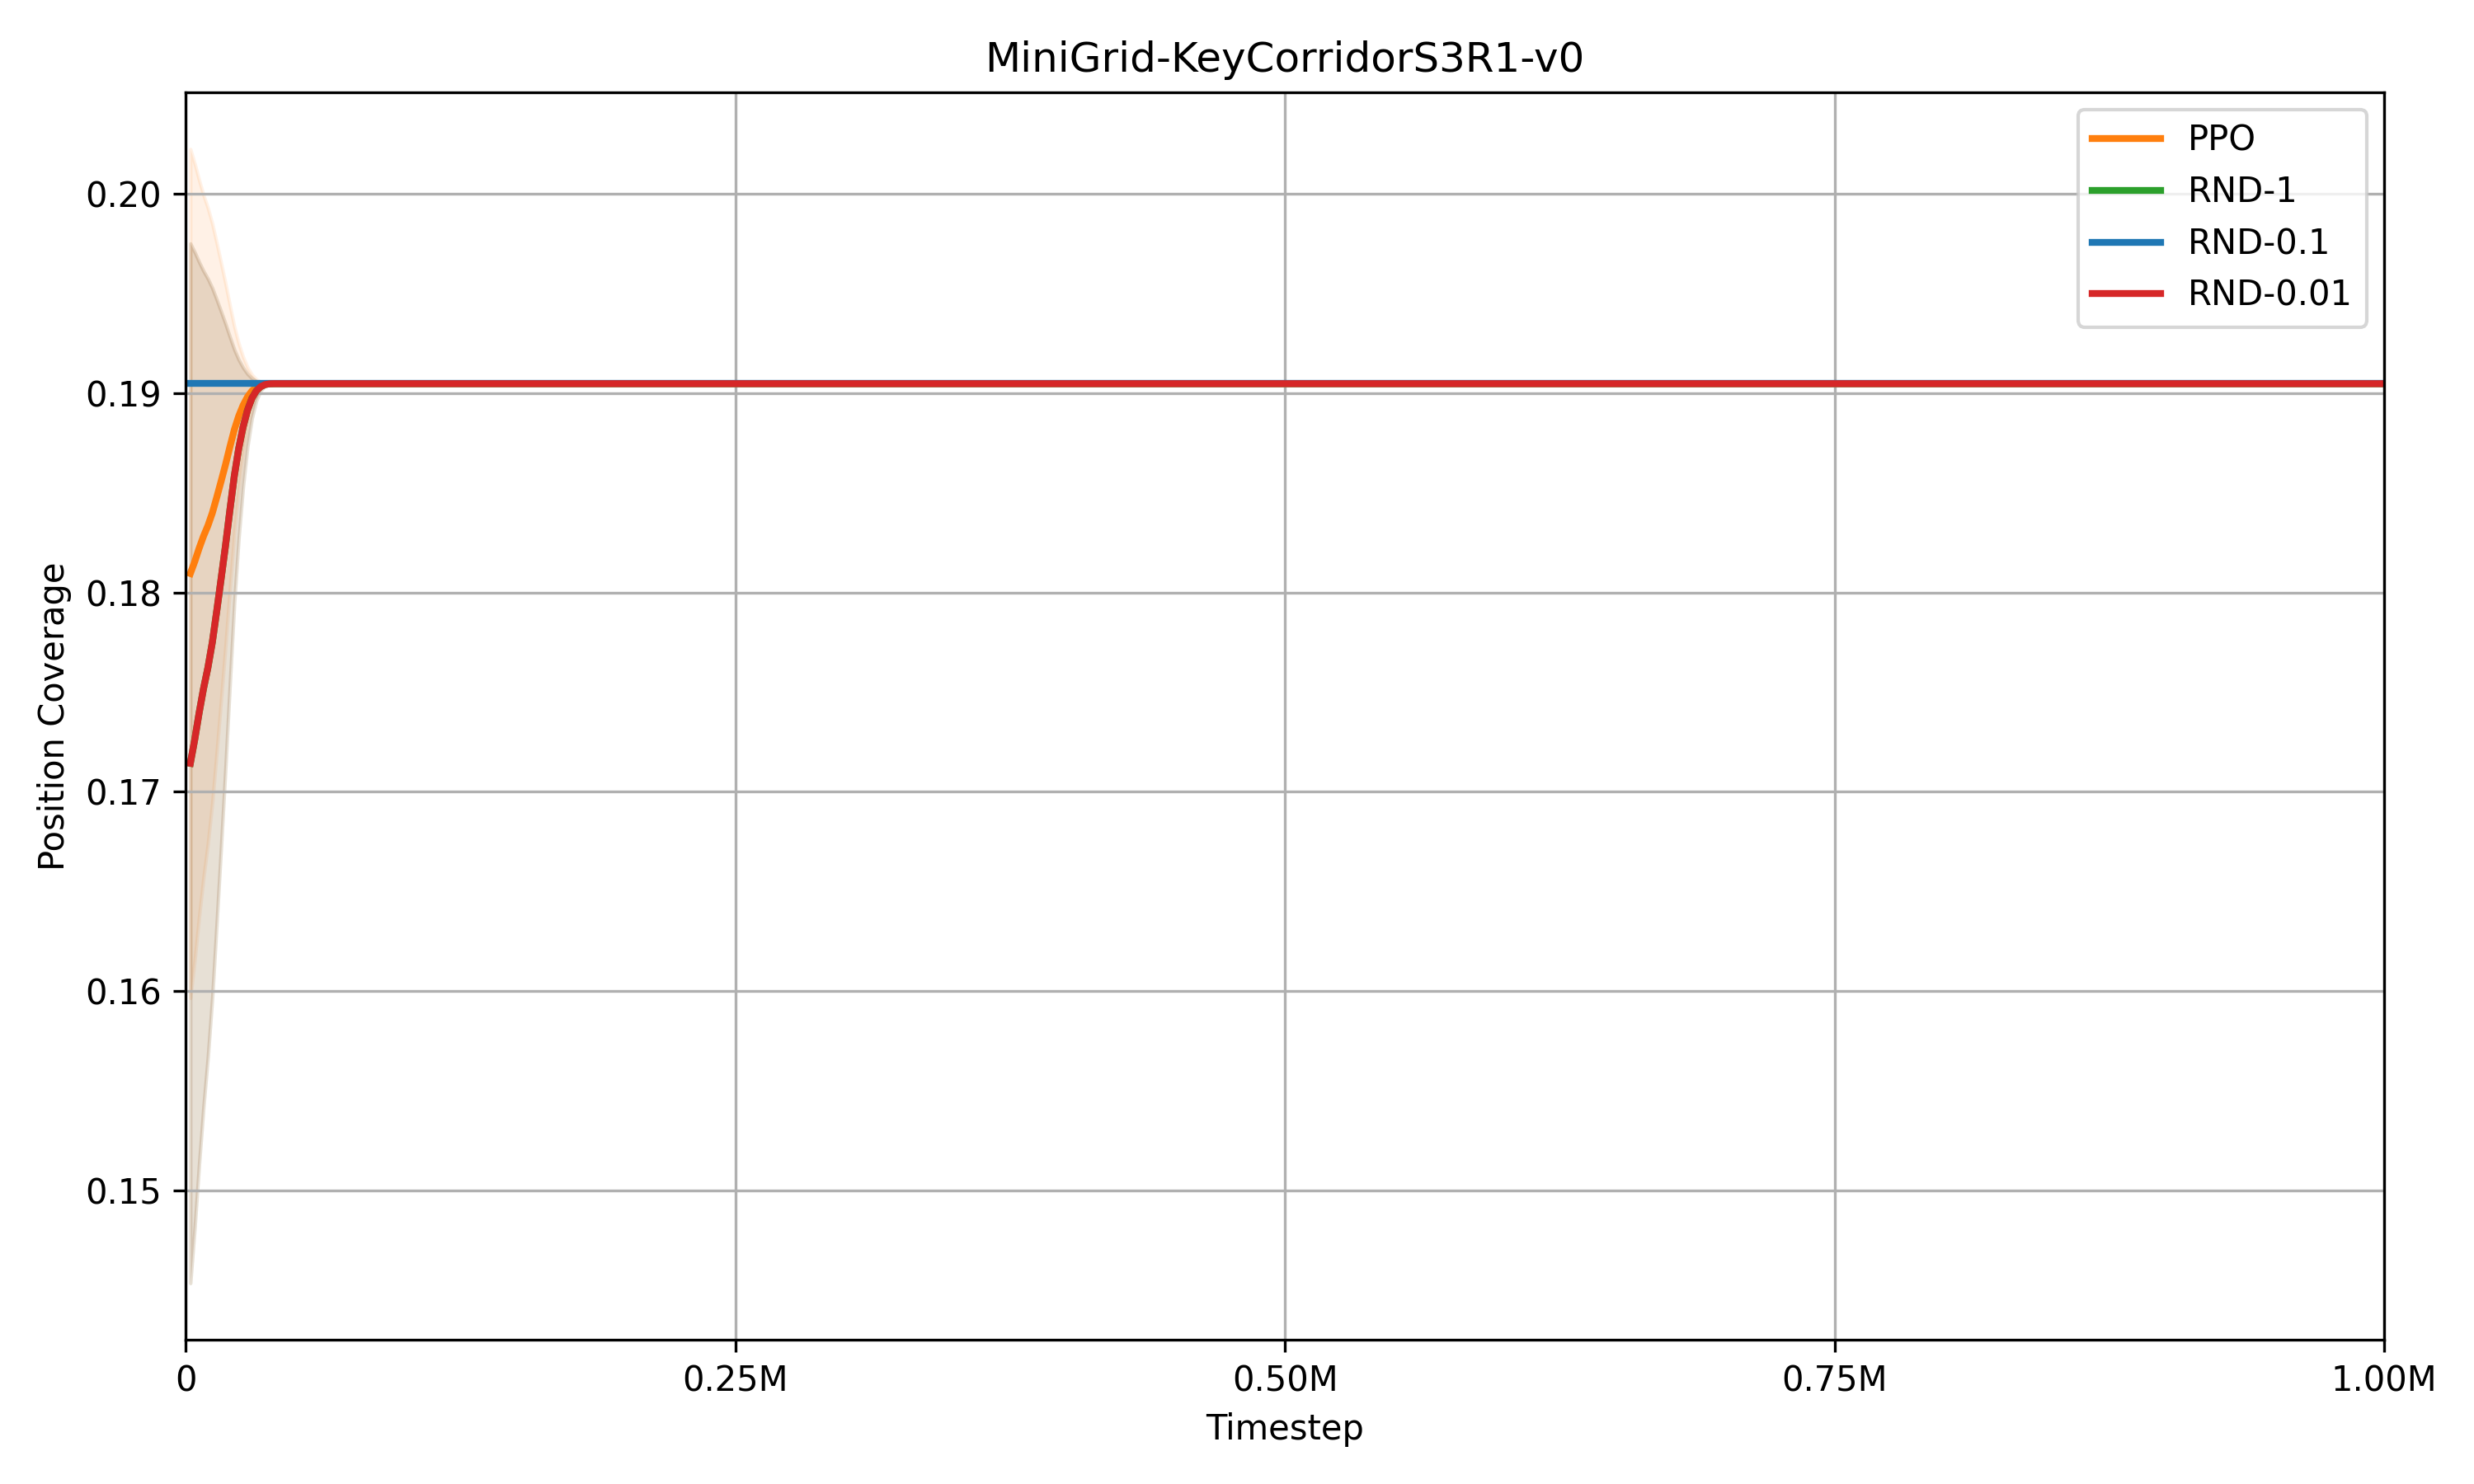
\includegraphics[width=\textwidth]{figs/MiniGrid-KeyCorridorS3R1-v0/pos_coverage.png}
    
    (c) Position Coverage
\end{minipage}
\hfill
\begin{minipage}{0.45\textwidth}
    \centering
    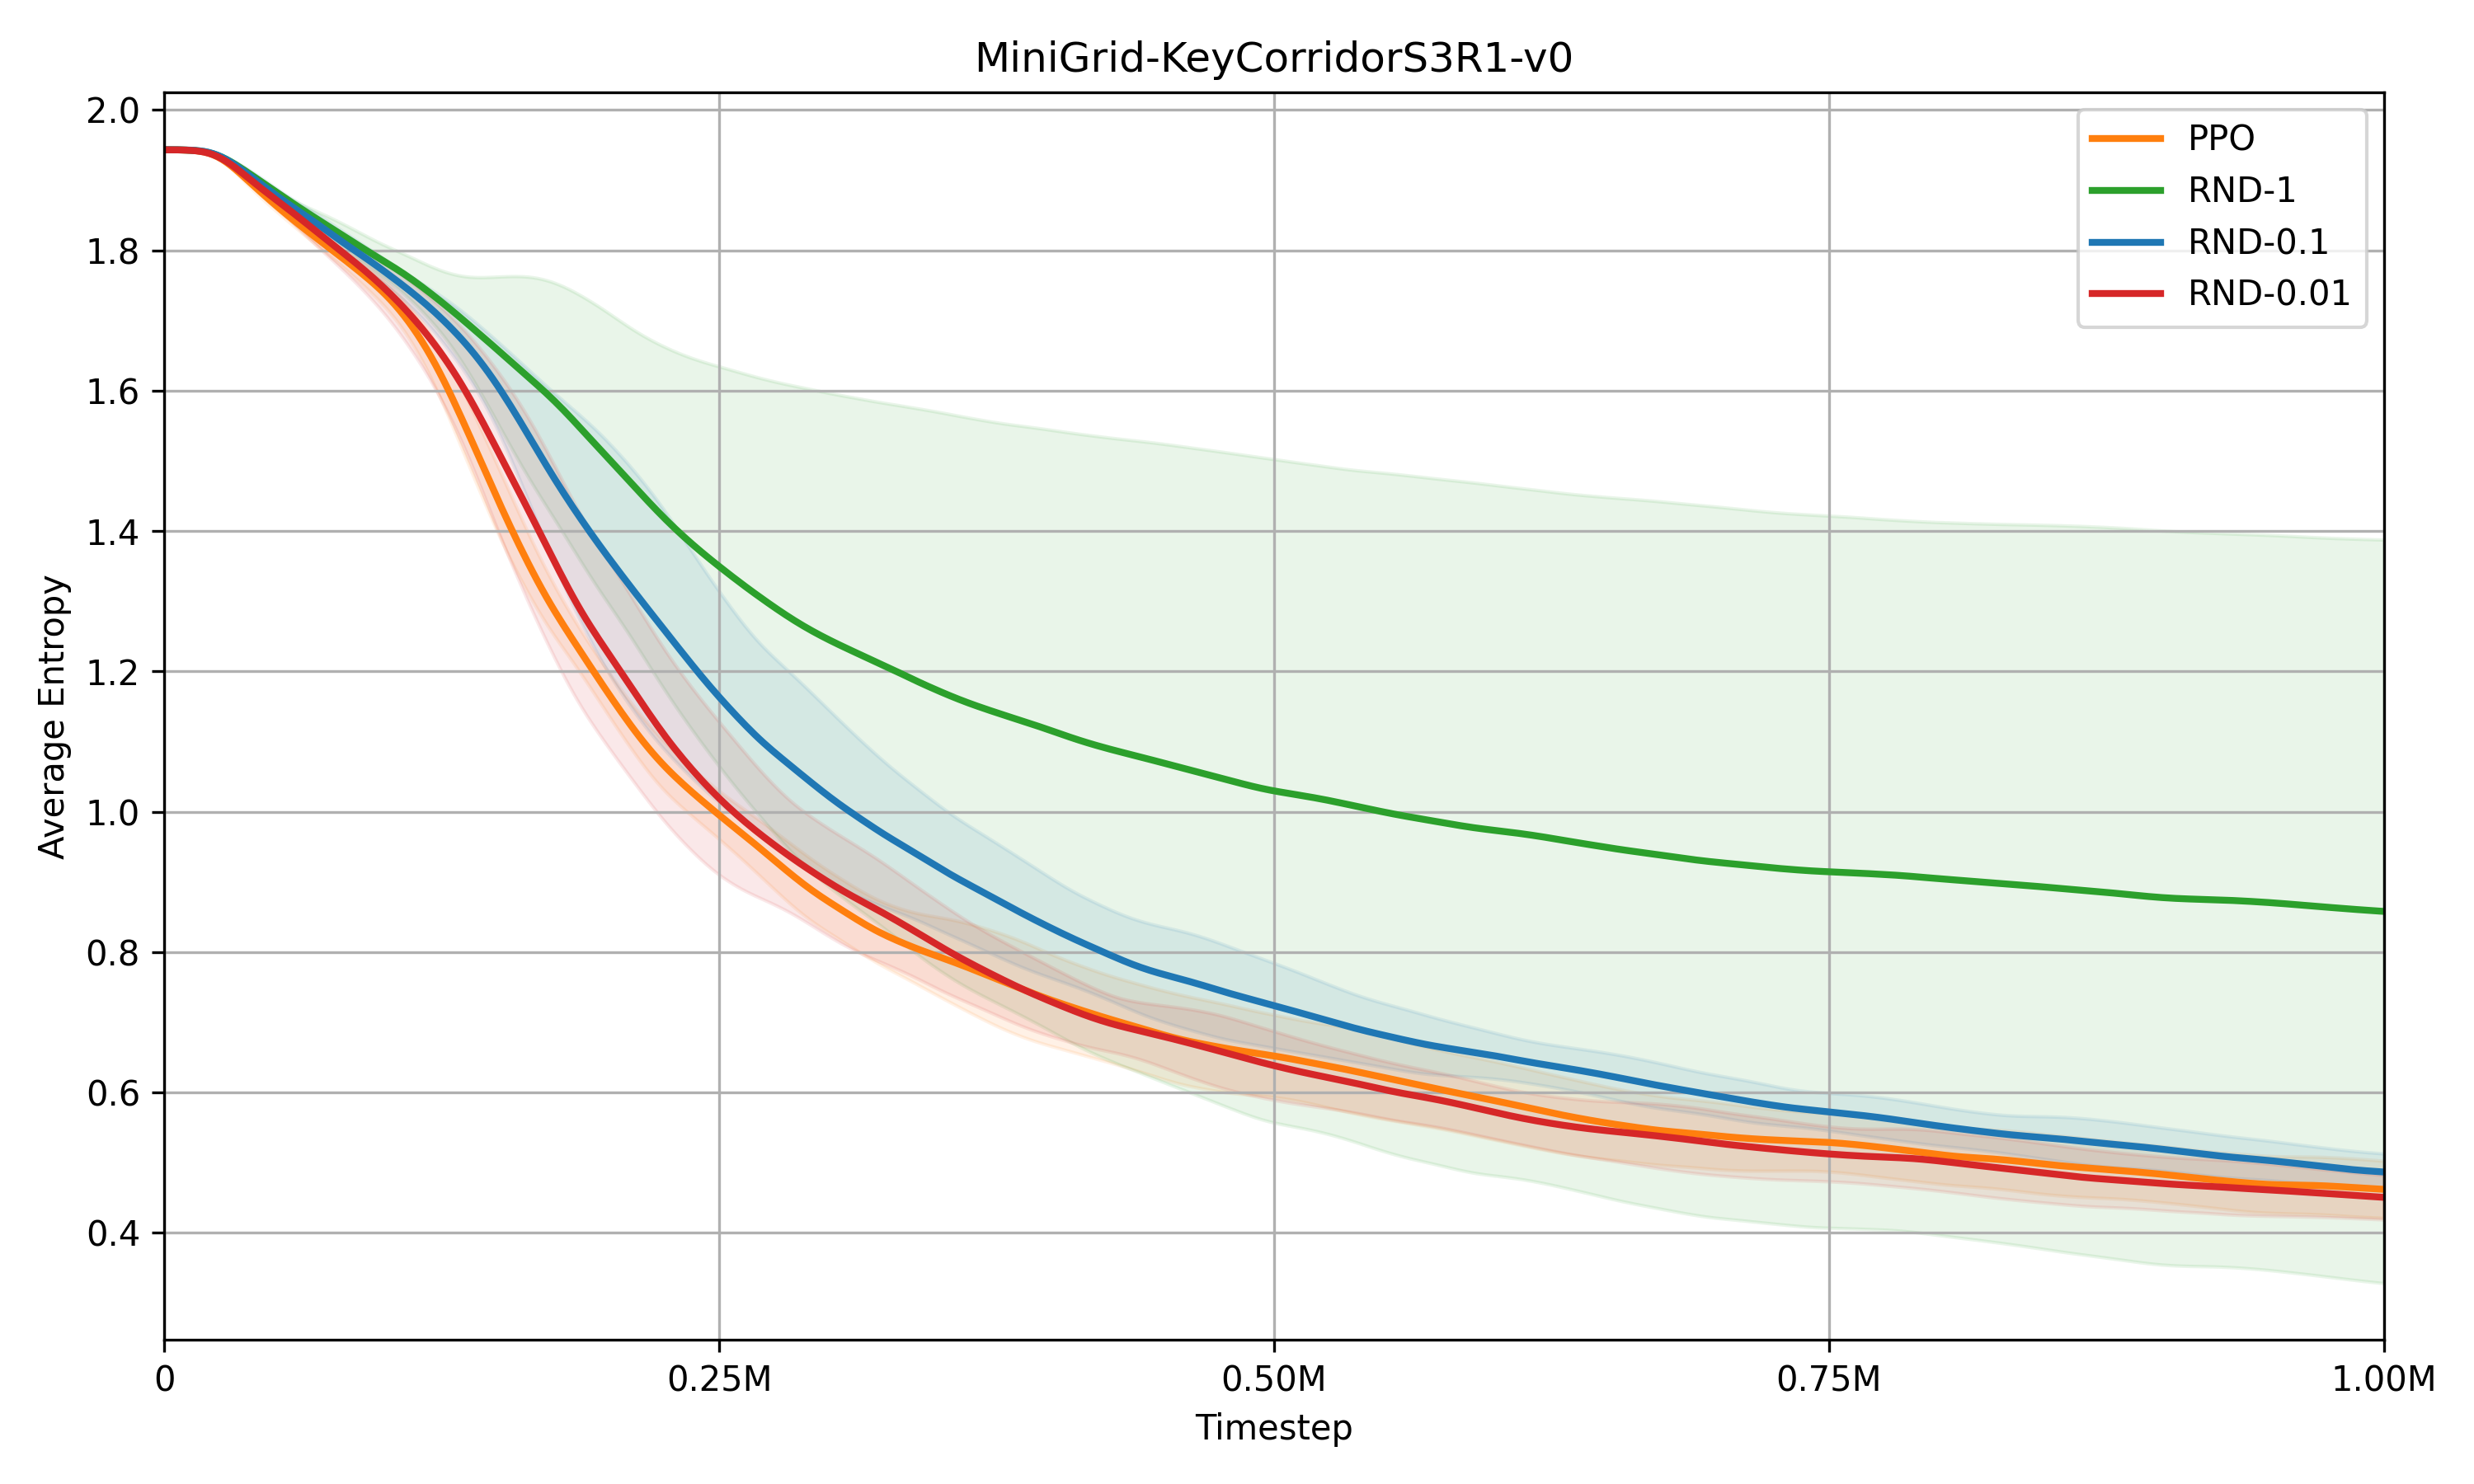
\includegraphics[width=\textwidth]{figs/MiniGrid-KeyCorridorS3R1-v0/avg_entropy.png}
    
    (d) Policy Entropy
\end{minipage}
\end{figure}

\begin{figure}[H]{Các chỉ số huấn luyện trên KeyCorridor-S3R2}
\centering
\begin{minipage}{0.45\textwidth}
    \centering
    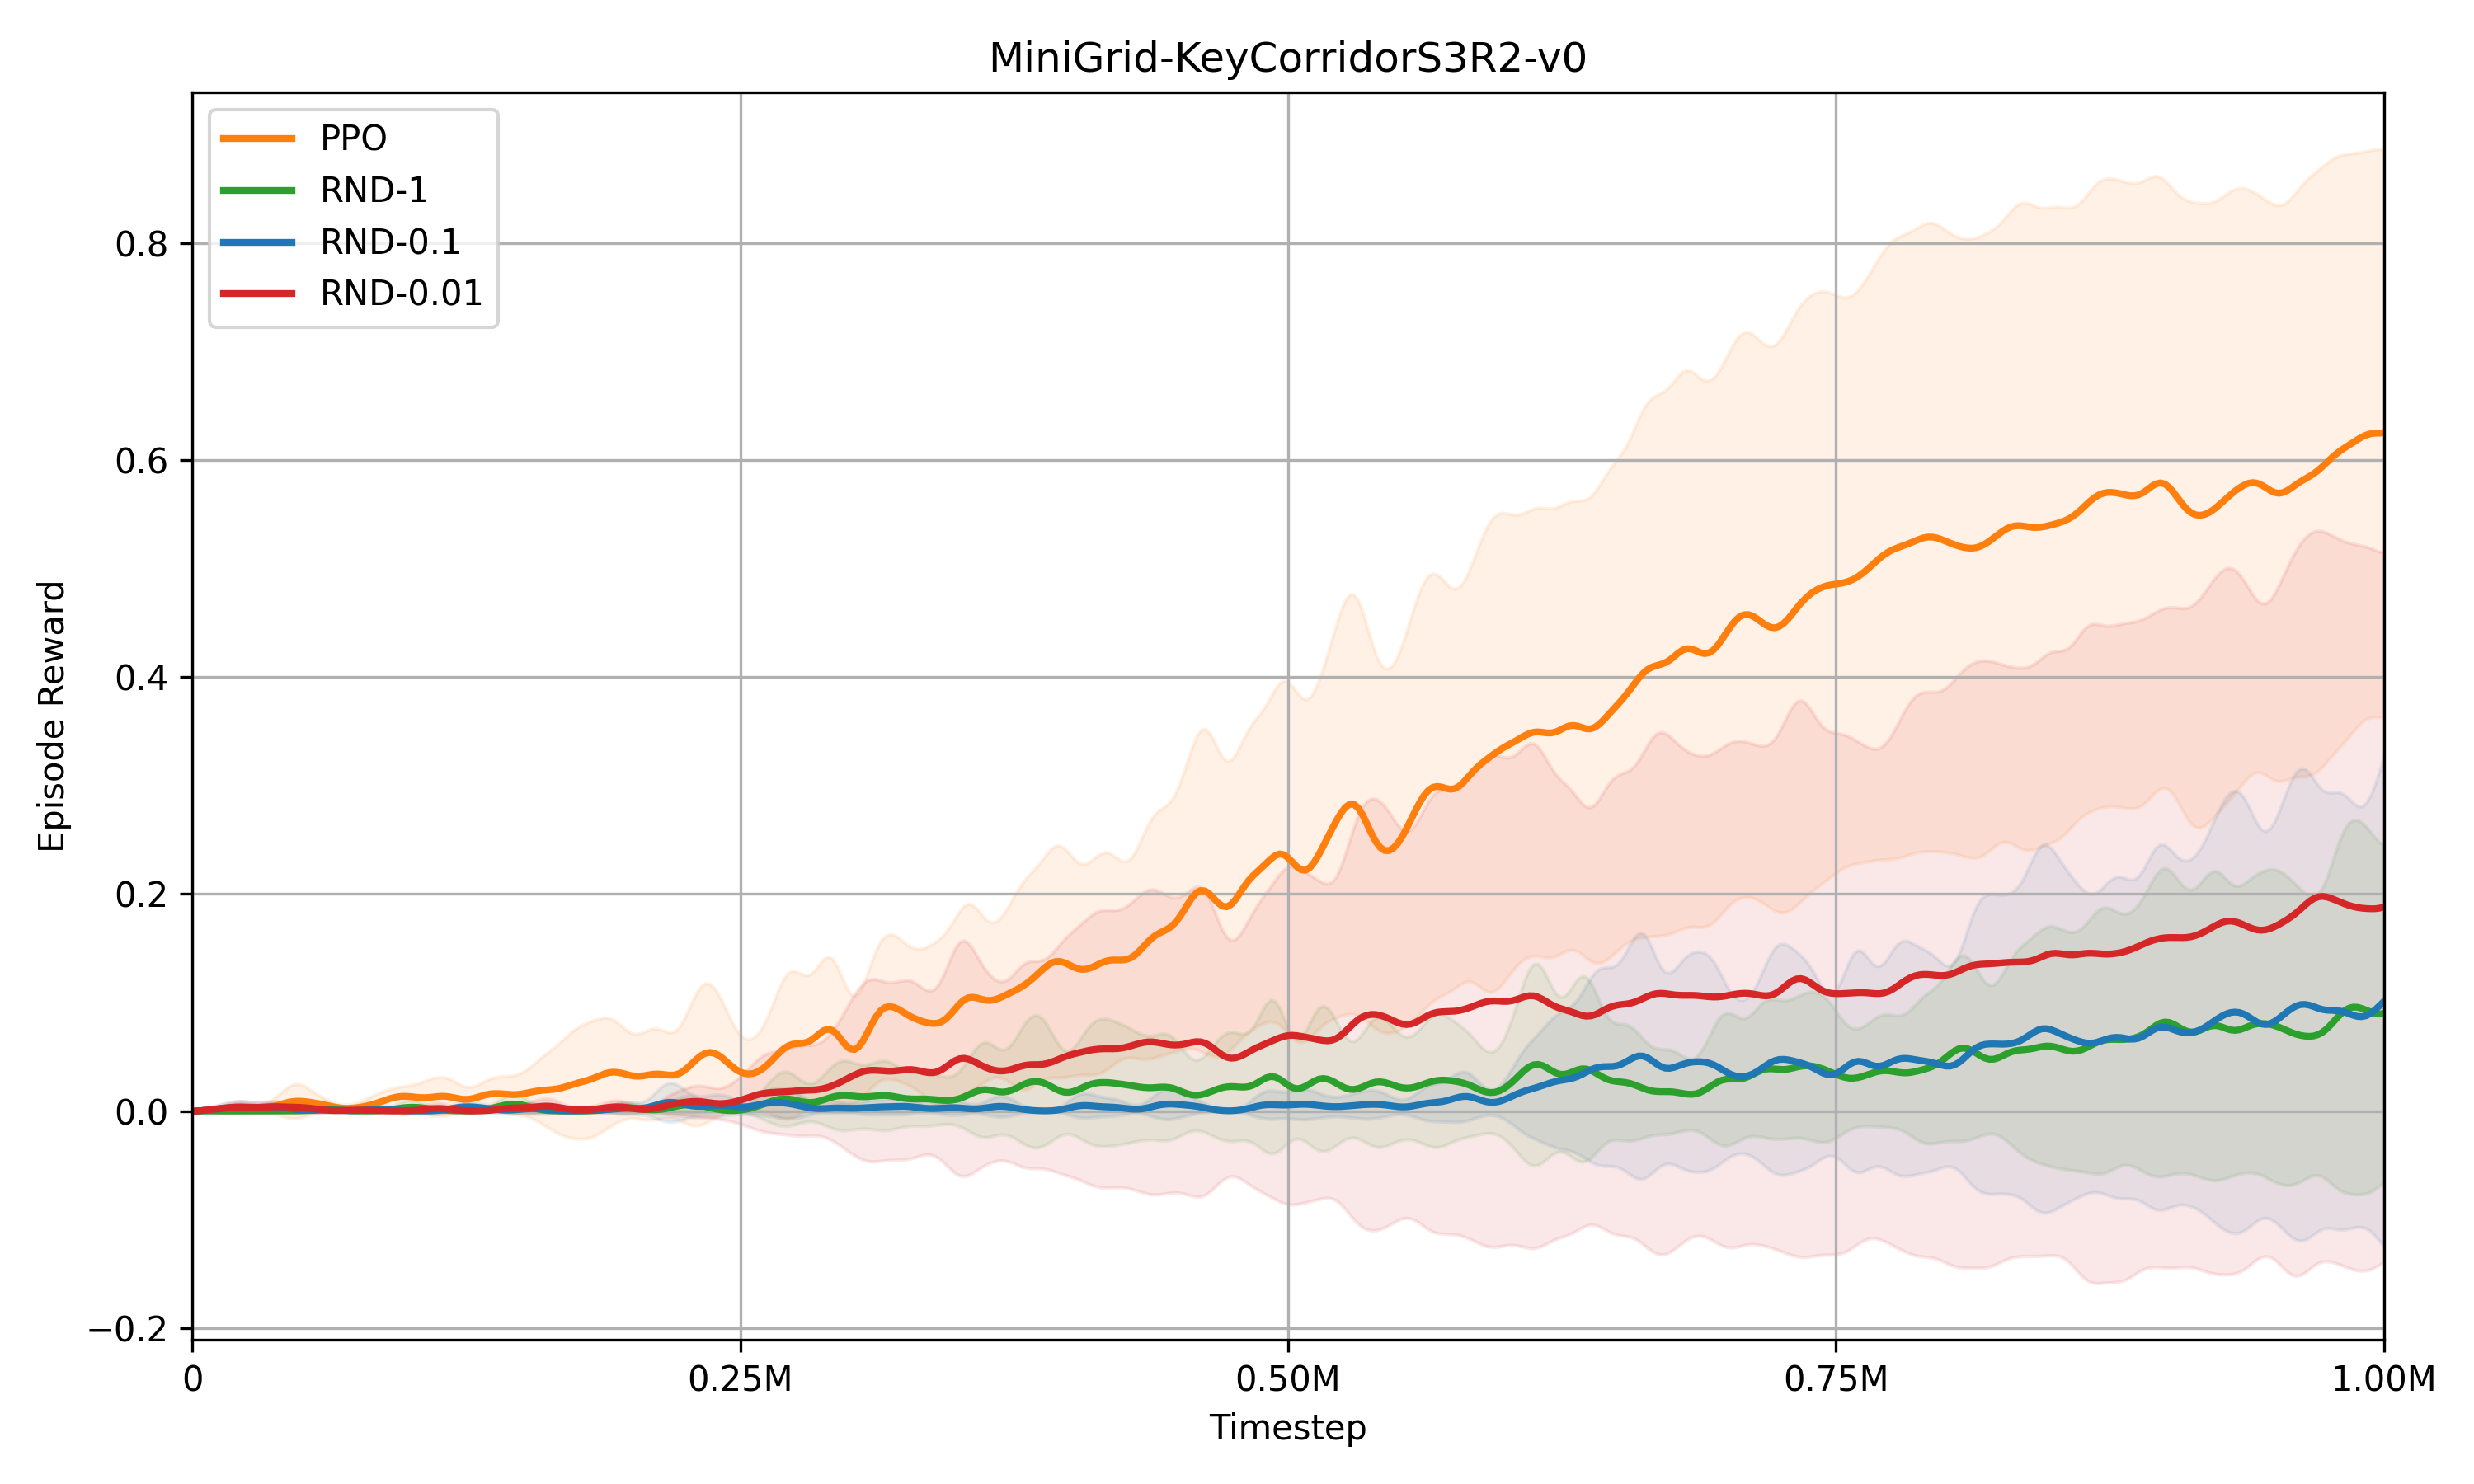
\includegraphics[width=\textwidth]{figs/MiniGrid-KeyCorridorS3R2-v0/episode_reward.png}
    
    (a) Episode Reward
\end{minipage}
\hfill
\begin{minipage}{0.45\textwidth}
    \centering
    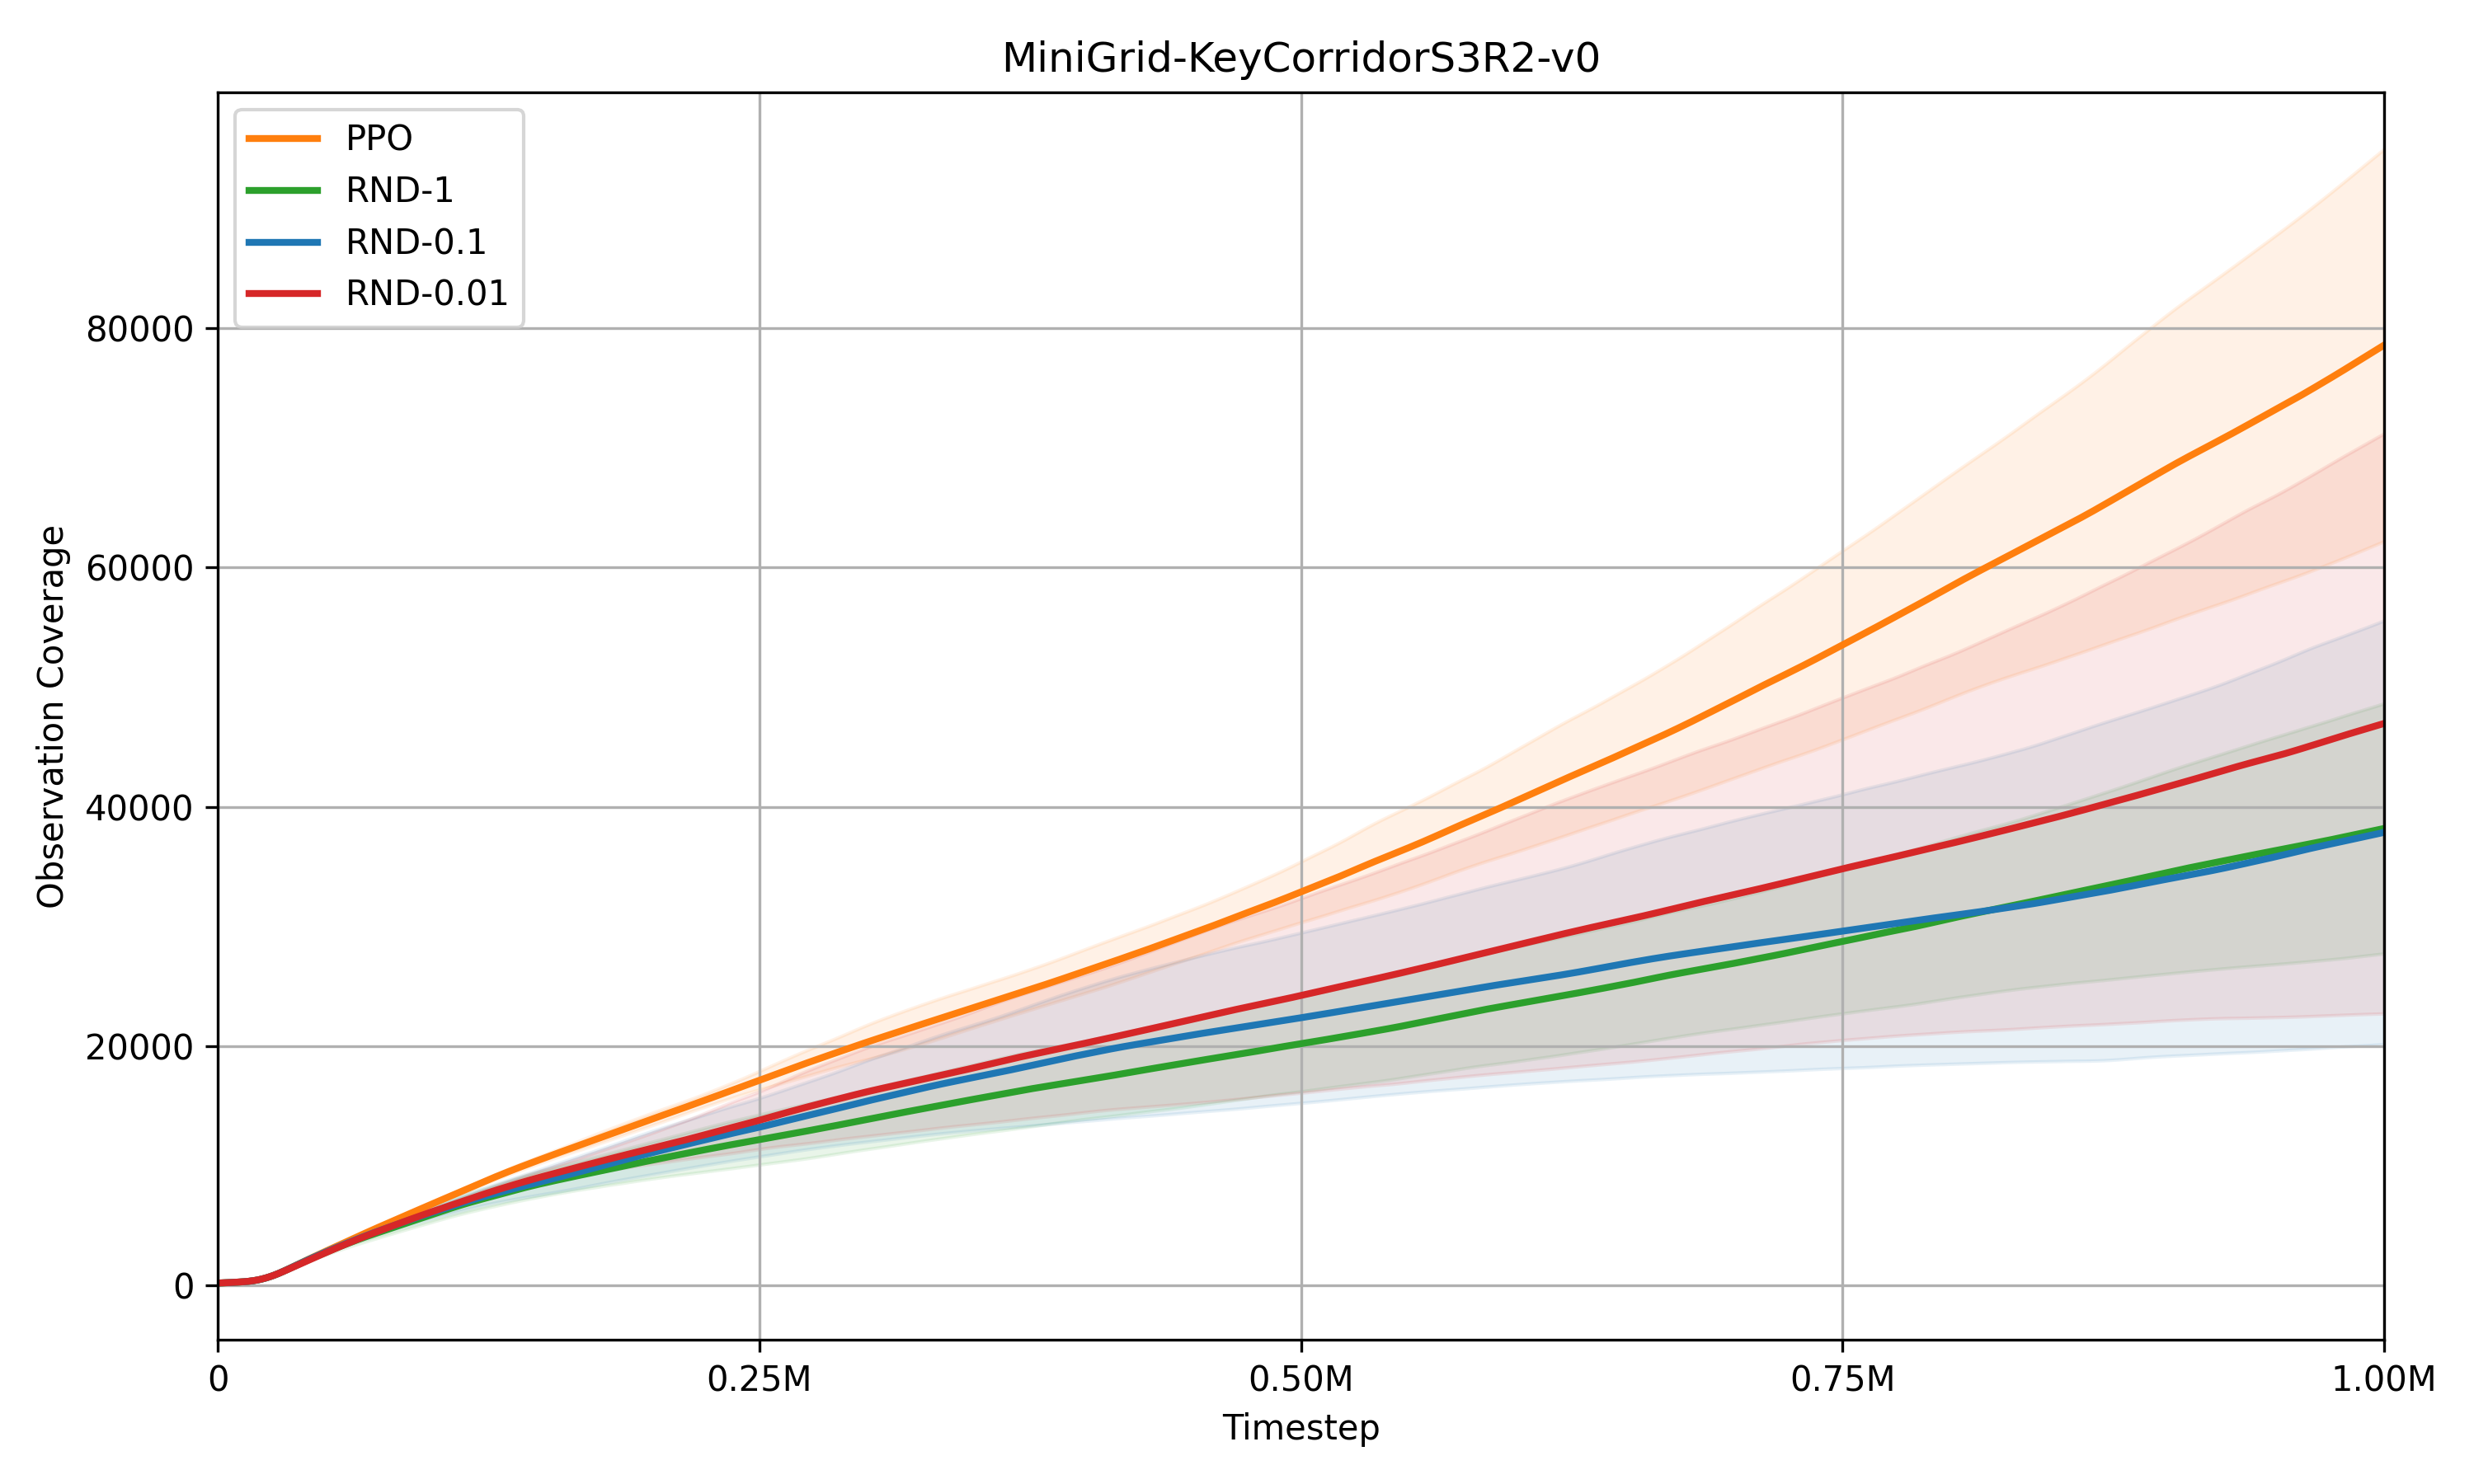
\includegraphics[width=\textwidth]{figs/MiniGrid-KeyCorridorS3R2-v0/obs_coverage.png}
    
    (b) Observation Coverage
\end{minipage}

\vspace{0.3cm}

\begin{minipage}{0.45\textwidth}
    \centering
    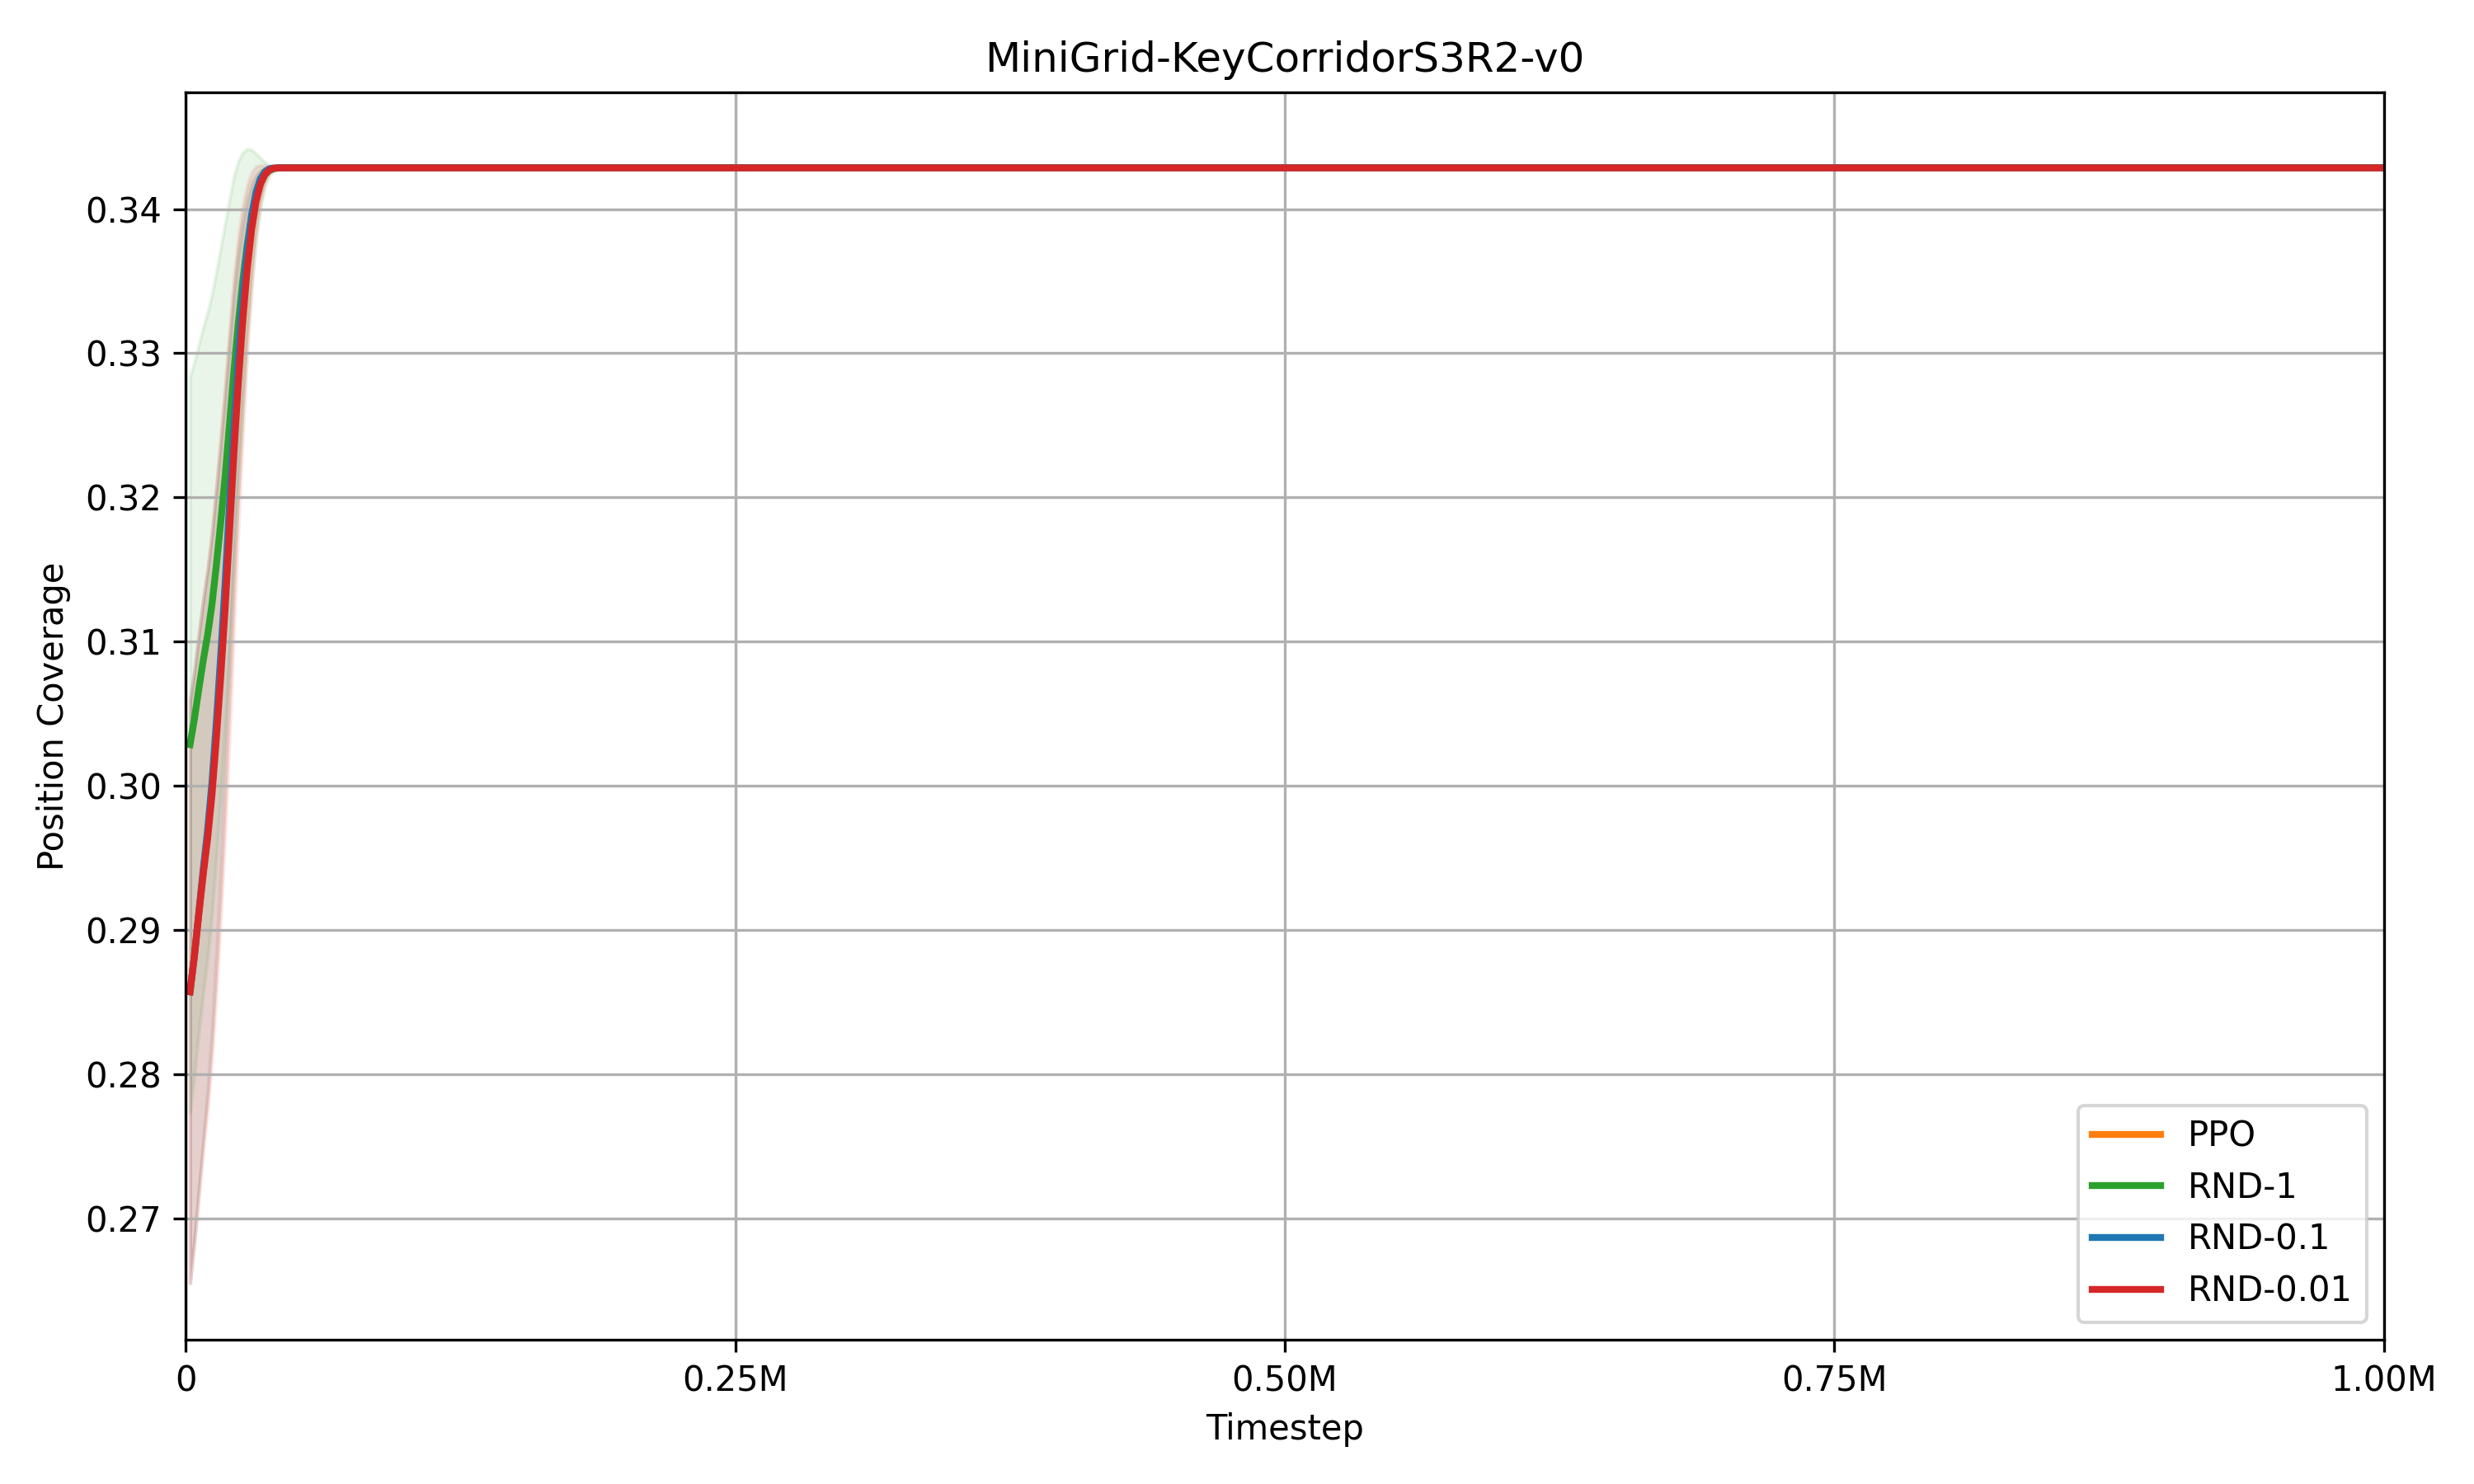
\includegraphics[width=\textwidth]{figs/MiniGrid-KeyCorridorS3R2-v0/pos_coverage.png}
    
    (c) Position Coverage
\end{minipage}
\hfill
\begin{minipage}{0.45\textwidth}
    \centering
    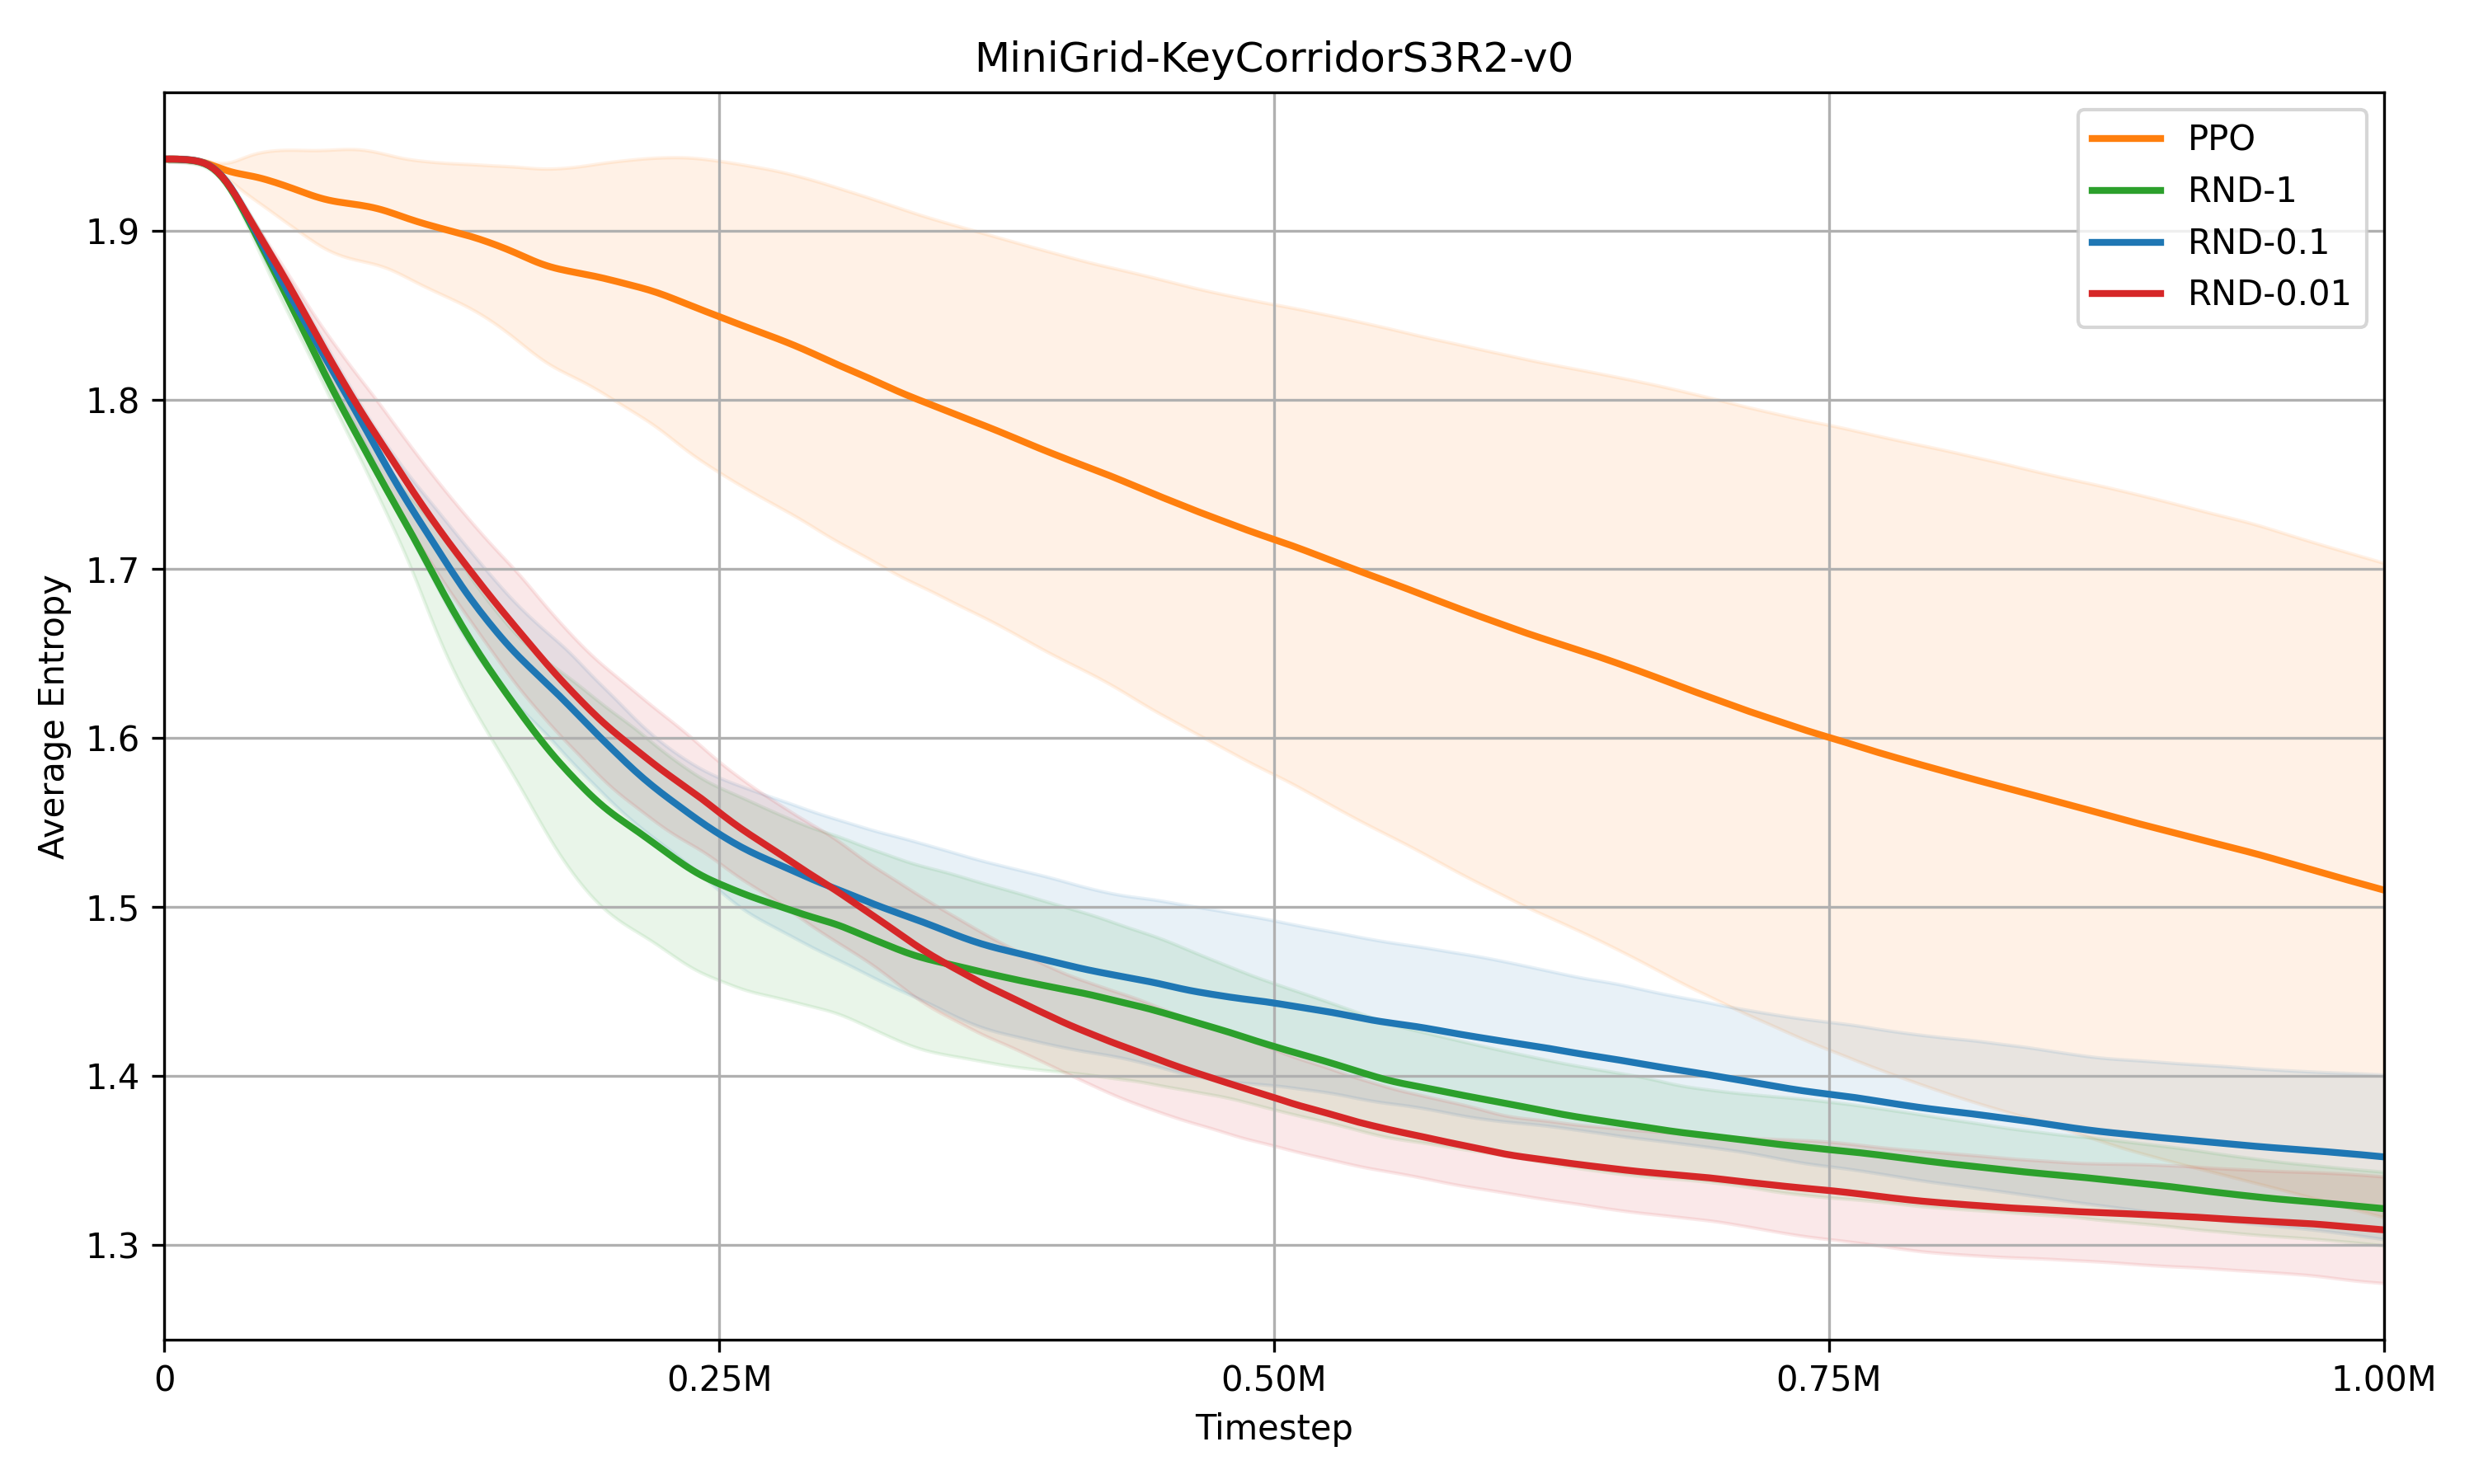
\includegraphics[width=\textwidth]{figs/MiniGrid-KeyCorridorS3R2-v0/avg_entropy.png}
    
    (d) Policy Entropy
\end{minipage}
\end{figure}

\subsection{Kết quả của RQ4}
% TODO: Viết nội dung

\section{Thảo luận kết quả}
% TODO: Viết nội dung

% =============================================
% CHƯƠNG 5: KẾT LUẬN
% =============================================
\chapter{Kết luận}

\section{Hạn chế}

Nghiên cứu này vẫn còn một số hạn chế cần được cải thiện:
\begin{itemize}
    \item Môi trường thử nghiệm: Các thực nghiệm chỉ được thực hiện trên môi trường MiniGrid với không gian trạng thái rời rạc và đơn giản. Khả năng mở rộng sang các môi trường phức tạp hơn (ví dụ: Atari, MuJoCo) chưa được kiểm chứng.
    \item Tối ưu hóa siêu tham số: Các siêu tham số được lựa chọn dựa trên kinh nghiệm và thử nghiệm thủ công, chưa áp dụng các phương pháp tự động hóa như Bayesian Optimization hay Population-Based Training.
    \item Chi phí tính toán: Việc duy trì và huấn luyện thêm mạng RND làm tăng chi phí tính toán so với PPO thuần túy.
\end{itemize}

\section{Hướng phát triển}

Dựa trên kết quả và hạn chế của nghiên cứu, em đề xuất các hướng phát triển sau:

\subsection{Mở rộng sang hệ thống đa tác tử (Multi-Agent RL)}

Hướng phát triển chính trong tương lai là mở rộng nghiên cứu sang bài toán học tăng cường đa tác tử (Multi-Agent Reinforcement Learning - MARL). Trong môi trường đa tác tử, vấn đề khám phá trở nên phức tạp hơn do:
\begin{itemize}
    \item Không gian trạng thái-hành động mở rộng: Với $n$ tác tử, không gian hành động chung tăng theo cấp số mũ, làm tăng độ khó của bài toán khám phá.
    \item Tín hiệu phần thưởng không tĩnh (Non-stationarity): Môi trường thay đổi liên tục do hành động của các tác tử khác, khiến việc học trở nên khó khăn hơn.
    \item Bài toán gán công trạng (Credit Assignment): Khó xác định đóng góp của từng tác tử trong phần thưởng chung của nhóm.
\end{itemize}

Trong bối cảnh MARL, việc nhiều tác tử cùng khám phá sẽ làm thay đổi trạng thái môi trường liên tục (non-stationarity), khiến tín hiệu RND của từng cá nhân bị nhiễu nghiêm trọng: một trạng thái ``mới lạ'' với tác tử A có thể là kết quả hành động của tác tử B, không phải do tác tử A khám phá. Do đó, các hướng nghiên cứu tiềm năng bao gồm:

\begin{itemize}
    \item Centralized RND: Xây dựng mạng RND tập trung dựa trên trạng thái toàn cục (global state), thay vì trạng thái cục bộ của từng tác tử. Cơ chế này giúp sinh phần thưởng nội tại nhất quán và tránh việc nhiều tác tử ``tranh giành'' khám phá cùng một vùng trạng thái.
    \item Chia sẻ tri thức khám phá (Exploration Knowledge Sharing): Các tác tử có thể chia sẻ bộ nhớ (memory) hoặc gradient của mạng Predictor để học chung từ kinh nghiệm khám phá của nhau, giảm thiểu việc lặp lại khám phá không cần thiết.
    \item Kết hợp với MAPPO/HAPPO: Tích hợp RND vào các thuật toán MARL hiện đại như Multi-Agent PPO (MAPPO) hoặc Heterogeneous-Agent PPO (HAPPO) để cải thiện khả năng phối hợp trong các nhiệm vụ có phần thưởng thưa.
\end{itemize}

\subsection{Các hướng phát triển khác}

\begin{itemize}
    \item Adaptive $\lambda$ Scheduling: Phát triển cơ chế tự động điều chỉnh hệ số $\lambda$ trong quá trình huấn luyện, giảm dần khi tác tử đã khám phá đủ và cần tập trung vào nhiệm vụ.
    
    \item Kết hợp với các phương pháp khám phá khác: Tích hợp RND với các kỹ thuật như ICM (Intrinsic Curiosity Module), count-based exploration, hoặc Go-Explore để tận dụng ưu điểm của từng phương pháp.
    
    \item Áp dụng vào bài toán thực tế: Thử nghiệm trên các bài toán robot navigation, game AI, hoặc autonomous driving với phần thưởng thưa thớt.
\end{itemize}

% ---------------------------------------------
% 5. Tài liệu tham khảo
% ---------------------------------------------
\begin{thebibliography}{99}
\begin{bibsection}{Tiếng Anh}
\bibitem{kayal2025}
Aya Kayal, Eduardo Pignatelli, and Laura Toni.
\textit{The impact of intrinsic rewards on exploration in Reinforcement Learning}.
arXiv preprint arXiv:2501.11533, 2025.

\bibitem{schulman2017}
John Schulman, Filip Wolski, Prafulla Dhariwal, Alec Radford, and Oleg Klimov.
\textit{Proximal Policy Optimization Algorithms}.
arXiv preprint arXiv:1707.06347, 2017.

\bibitem{burda2019rnd}
Yuri Burda, Harrison Edwards, Amos Storkey, and Oleg Klimov.
\textit{Exploration by Random Network Distillation}.
International Conference on Learning Representations (ICLR), 2019.

\bibitem{burda2019curiosity}
Yuri Burda, Harrison Edwards, Deepak Pathak, Amos Storkey, Trevor Darrell, and Alexei~A. Efros.
\textit{Large-Scale Study of Curiosity-Driven Learning}.
International Conference on Learning Representations (ICLR), 2019.

\bibitem{bellemare2016}
Marc~G. Bellemare, Sriram Srinivasan, Georg Ostrovski, Tom Schaul, David Saxton, and Rémi Munos.
\textit{Unifying Count-Based Exploration and Intrinsic Motivation}.
Advances in Neural Information Processing Systems (NeurIPS), 29, 2016.

\bibitem{chevalier2023}
Maxime Chevalier-Boisvert, Bolun Dai, Mark Towers, Rodrigo de Lazcano, Lucas Willems, Salem Lahlou, Suman Pal, Pablo~Samuel Castro, and Jordan Terry.
\textit{Minigrid \& Miniworld: Modular \& Customizable Reinforcement Learning Environments for Goal-Oriented Tasks}.
Advances in Neural Information Processing Systems (NeurIPS), 36, 2023.

\bibitem{eysenbach2019}
Benjamin Eysenbach, Abhishek Gupta, Julian Ibarz, and Sergey Levine.
\textit{Diversity is All You Need: Learning Skills without a Reward Function}.
International Conference on Learning Representations (ICLR), 2019.

\bibitem{haarnoja2018}
Tuomas Haarnoja, Aurick Zhou, Pieter Abbeel, and Sergey Levine.
\textit{Soft Actor-Critic: Off-Policy Maximum Entropy Deep Reinforcement Learning with a Stochastic Actor}.
Proceedings of the 35th International Conference on Machine Learning (ICML), 1861--1870, 2018.

\bibitem{pathak2017}
Deepak Pathak, Pulkit Agrawal, Alexei~A. Efros, and Trevor Darrell.
\textit{Curiosity-driven Exploration by Self-supervised Prediction}.
Proceedings of the 34th International Conference on Machine Learning (ICML), 2778--2787, 2017.

\bibitem{schulman2015}
John Schulman, Sergey Levine, Pieter Abbeel, Michael Jordan, and Philipp Moritz.
\textit{Trust Region Policy Optimization}.
Proceedings of the 32nd International Conference on Machine Learning (ICML), 1889--1897, 2015.

\bibitem{sutton2018}
Richard~S. Sutton and Andrew~G. Barto.
\textit{Reinforcement Learning: An Introduction} (2nd ed.).
MIT Press, 2018.
\end{bibsection}
\end{thebibliography}

\end{document}